\documentclass[twoside]{book}

% Packages required by doxygen
\usepackage{calc}
\usepackage{doxygen}
\usepackage{graphicx}
\usepackage[utf8]{inputenc}
\usepackage{makeidx}
\usepackage{multicol}
\usepackage{multirow}
\usepackage{fixltx2e}
\PassOptionsToPackage{warn}{textcomp}
\usepackage{textcomp}
\usepackage[nointegrals]{wasysym}
\usepackage[table]{xcolor}

% Font selection
\usepackage[T1]{fontenc}
\usepackage{mathptmx}
\usepackage[scaled=.90]{helvet}
\usepackage{courier}
\usepackage{amssymb}
\usepackage{sectsty}
\renewcommand{\familydefault}{\sfdefault}
\allsectionsfont{%
  \fontseries{bc}\selectfont%
  \color{darkgray}%
}
\renewcommand{\DoxyLabelFont}{%
  \fontseries{bc}\selectfont%
  \color{darkgray}%
}
\newcommand{\+}{\discretionary{\mbox{\scriptsize$\hookleftarrow$}}{}{}}

% Page & text layout
\usepackage{geometry}
\geometry{%
  a4paper,%
  top=2.5cm,%
  bottom=2.5cm,%
  left=2.5cm,%
  right=2.5cm%
}
\tolerance=750
\hfuzz=15pt
\hbadness=750
\setlength{\emergencystretch}{15pt}
\setlength{\parindent}{0cm}
\setlength{\parskip}{0.2cm}
\makeatletter
\renewcommand{\paragraph}{%
  \@startsection{paragraph}{4}{0ex}{-1.0ex}{1.0ex}{%
    \normalfont\normalsize\bfseries\SS@parafont%
  }%
}
\renewcommand{\subparagraph}{%
  \@startsection{subparagraph}{5}{0ex}{-1.0ex}{1.0ex}{%
    \normalfont\normalsize\bfseries\SS@subparafont%
  }%
}
\makeatother

% Headers & footers
\usepackage{fancyhdr}
\pagestyle{fancyplain}
\fancyhead[LE]{\fancyplain{}{\bfseries\thepage}}
\fancyhead[CE]{\fancyplain{}{}}
\fancyhead[RE]{\fancyplain{}{\bfseries\leftmark}}
\fancyhead[LO]{\fancyplain{}{\bfseries\rightmark}}
\fancyhead[CO]{\fancyplain{}{}}
\fancyhead[RO]{\fancyplain{}{\bfseries\thepage}}
\fancyfoot[LE]{\fancyplain{}{}}
\fancyfoot[CE]{\fancyplain{}{}}
\fancyfoot[RE]{\fancyplain{}{\bfseries\scriptsize Generated on Mon Aug 18 2014 09\+:23\+:36 for T\+S\+G\+L by Doxygen }}
\fancyfoot[LO]{\fancyplain{}{\bfseries\scriptsize Generated on Mon Aug 18 2014 09\+:23\+:36 for T\+S\+G\+L by Doxygen }}
\fancyfoot[CO]{\fancyplain{}{}}
\fancyfoot[RO]{\fancyplain{}{}}
\renewcommand{\footrulewidth}{0.4pt}
\renewcommand{\chaptermark}[1]{%
  \markboth{#1}{}%
}
\renewcommand{\sectionmark}[1]{%
  \markright{\thesection\ #1}%
}

% Indices & bibliography
\usepackage{natbib}
\usepackage[titles]{tocloft}
\setcounter{tocdepth}{3}
\setcounter{secnumdepth}{5}
\makeindex

% Hyperlinks (required, but should be loaded last)
\usepackage{ifpdf}
\ifpdf
  \usepackage[pdftex,pagebackref=true]{hyperref}
\else
  \usepackage[ps2pdf,pagebackref=true]{hyperref}
\fi
\hypersetup{%
  colorlinks=true,%
  linkcolor=blue,%
  citecolor=blue,%
  unicode%
}

% Custom commands
\newcommand{\clearemptydoublepage}{%
  \newpage{\pagestyle{empty}\cleardoublepage}%
}


%===== C O N T E N T S =====

\begin{document}

% Titlepage & ToC
\hypersetup{pageanchor=false,
             bookmarks=true,
             bookmarksnumbered=true,
             pdfencoding=unicode
            }
\pagenumbering{roman}
\begin{titlepage}
\vspace*{7cm}
\begin{center}%
{\Large T\+S\+G\+L }\\
\vspace*{1cm}
{\large Generated by Doxygen 1.8.7}\\
\vspace*{0.5cm}
{\small Mon Aug 18 2014 09:23:36}\\
\end{center}
\end{titlepage}
\clearemptydoublepage
\tableofcontents
\clearemptydoublepage
\pagenumbering{arabic}
\hypersetup{pageanchor=true}

%--- Begin generated contents ---
\chapter{Bug List}
\label{bug}
\hypertarget{bug}{}

\begin{DoxyRefList}
\item[\label{bug__bug000001}%
\hypertarget{bug__bug000001}{}%
Member \hyperlink{classtsgl_1_1_canvas_ac035f43763b198f6915a0772973a5ea9}{tsgl\+:\+:Canvas\+:\+:take\+Screen\+Shot} ()]Multiple calls to this function in rapid succession seem to make the F\+P\+S counter inaccurate.  
\item[\label{bug__bug000002}%
\hypertarget{bug__bug000002}{}%
Member \hyperlink{classtsgl_1_1_texture_handler_a7f3103ea7f43f5a042609b443a748c88}{tsgl\+:\+:Texture\+Handler\+:\+:draw\+Text} (std\+::wstring text, unsigned int font\+\_\+size, float $\ast$vertices)]If the default font cannot be located, T\+S\+G\+L will crash. 
\end{DoxyRefList}
\chapter{Hierarchical Index}
\section{Class Hierarchy}
This inheritance list is sorted roughly, but not completely, alphabetically\+:\begin{DoxyCompactList}
\item \contentsline{section}{tsgl\+:\+:Array$<$ Item $>$}{\pageref{classtsgl_1_1_array}}{}
\item \contentsline{section}{tsgl\+:\+:Array$<$ tsgl\+:\+:Shape $\ast$ $>$}{\pageref{classtsgl_1_1_array}}{}
\item \contentsline{section}{tsgl\+:\+:Canvas}{\pageref{classtsgl_1_1_canvas}}{}
\begin{DoxyCompactList}
\item \contentsline{section}{tsgl\+:\+:Cartesian\+Canvas}{\pageref{classtsgl_1_1_cartesian_canvas}}{}
\end{DoxyCompactList}
\item \contentsline{section}{tsgl\+:\+:Color\+Float}{\pageref{structtsgl_1_1_color_float}}{}
\item \contentsline{section}{tsgl\+:\+:Color\+H\+S\+V}{\pageref{structtsgl_1_1_color_h_s_v}}{}
\item \contentsline{section}{tsgl\+:\+:Color\+Int}{\pageref{structtsgl_1_1_color_int}}{}
\item \contentsline{section}{tsgl\+:\+:Colors}{\pageref{classtsgl_1_1_colors}}{}
\item \contentsline{section}{tsgl\+:\+:Function}{\pageref{classtsgl_1_1_function}}{}
\begin{DoxyCompactList}
\item \contentsline{section}{tsgl\+:\+:Absolute\+Function}{\pageref{classtsgl_1_1_absolute_function}}{}
\item \contentsline{section}{tsgl\+:\+:Ceiling\+Function}{\pageref{classtsgl_1_1_ceiling_function}}{}
\item \contentsline{section}{tsgl\+:\+:Common\+Log\+Function}{\pageref{classtsgl_1_1_common_log_function}}{}
\item \contentsline{section}{tsgl\+:\+:Cosine\+Function}{\pageref{classtsgl_1_1_cosine_function}}{}
\item \contentsline{section}{tsgl\+:\+:Exponential\+Function}{\pageref{classtsgl_1_1_exponential_function}}{}
\item \contentsline{section}{tsgl\+:\+:Floor\+Function}{\pageref{classtsgl_1_1_floor_function}}{}
\item \contentsline{section}{tsgl\+:\+:Natural\+Log\+Function}{\pageref{classtsgl_1_1_natural_log_function}}{}
\item \contentsline{section}{tsgl\+:\+:Power\+Function}{\pageref{classtsgl_1_1_power_function}}{}
\item \contentsline{section}{tsgl\+:\+:Round\+Function}{\pageref{classtsgl_1_1_round_function}}{}
\item \contentsline{section}{tsgl\+:\+:Sine\+Function}{\pageref{classtsgl_1_1_sine_function}}{}
\item \contentsline{section}{tsgl\+:\+:Square\+Root\+Function}{\pageref{classtsgl_1_1_square_root_function}}{}
\item \contentsline{section}{tsgl\+:\+:Tangent\+Function}{\pageref{classtsgl_1_1_tangent_function}}{}
\end{DoxyCompactList}
\item \contentsline{section}{tsgl\+:\+:Progress\+Bar}{\pageref{classtsgl_1_1_progress_bar}}{}
\item \contentsline{section}{tsgl\+:\+:Shape}{\pageref{classtsgl_1_1_shape}}{}
\begin{DoxyCompactList}
\item \contentsline{section}{tsgl\+:\+:Colored\+Polygon}{\pageref{classtsgl_1_1_colored_polygon}}{}
\item \contentsline{section}{tsgl\+:\+:Concave\+Polygon}{\pageref{classtsgl_1_1_concave_polygon}}{}
\item \contentsline{section}{tsgl\+:\+:Convex\+Polygon}{\pageref{classtsgl_1_1_convex_polygon}}{}
\item \contentsline{section}{tsgl\+:\+:Image}{\pageref{classtsgl_1_1_image}}{}
\item \contentsline{section}{tsgl\+:\+:Line}{\pageref{classtsgl_1_1_line}}{}
\item \contentsline{section}{tsgl\+:\+:Polyline}{\pageref{classtsgl_1_1_polyline}}{}
\item \contentsline{section}{tsgl\+:\+:Rectangle}{\pageref{classtsgl_1_1_rectangle}}{}
\item \contentsline{section}{tsgl\+:\+:Text}{\pageref{classtsgl_1_1_text}}{}
\item \contentsline{section}{tsgl\+:\+:Triangle}{\pageref{classtsgl_1_1_triangle}}{}
\end{DoxyCompactList}
\item \contentsline{section}{tsgl\+:\+:Spectrogram}{\pageref{classtsgl_1_1_spectrogram}}{}
\item \contentsline{section}{tsgl\+:\+:Texture\+Handler}{\pageref{classtsgl_1_1_texture_handler}}{}
\item \contentsline{section}{tsgl\+:\+:Timer}{\pageref{classtsgl_1_1_timer}}{}
\item \contentsline{section}{tsgl\+:\+:Visual\+Task\+Queue}{\pageref{classtsgl_1_1_visual_task_queue}}{}
\end{DoxyCompactList}

\chapter{Class Index}
\section{Class List}
Here are the classes, structs, unions and interfaces with brief descriptions\+:\begin{DoxyCompactList}
\item\contentsline{section}{\hyperlink{classtsgl_1_1_absolute_function}{tsgl\+::\+Absolute\+Function} \\*\hyperlink{classtsgl_1_1_function}{Function} to compute the absolute value of the input }{\pageref{classtsgl_1_1_absolute_function}}{}
\item\contentsline{section}{\hyperlink{classtsgl_1_1_array}{tsgl\+::\+Array$<$ Item $>$} \\*Custom internal array used by \hyperlink{classtsgl_1_1_canvas}{Canvas} }{\pageref{classtsgl_1_1_array}}{}
\item\contentsline{section}{\hyperlink{classtsgl_1_1_canvas}{tsgl\+::\+Canvas} \\*A G\+L window with numerous built-\/in, thread-\/safe drawing operations }{\pageref{classtsgl_1_1_canvas}}{}
\item\contentsline{section}{\hyperlink{classtsgl_1_1_cartesian_canvas}{tsgl\+::\+Cartesian\+Canvas} \\*\hyperlink{classtsgl_1_1_canvas}{Canvas} extended for graphic support }{\pageref{classtsgl_1_1_cartesian_canvas}}{}
\item\contentsline{section}{\hyperlink{classtsgl_1_1_ceiling_function}{tsgl\+::\+Ceiling\+Function} \\*\hyperlink{classtsgl_1_1_function}{Function} to compute the mathematical ceiling of the input }{\pageref{classtsgl_1_1_ceiling_function}}{}
\item\contentsline{section}{\hyperlink{classtsgl_1_1_colored_polygon}{tsgl\+::\+Colored\+Polygon} \\*Draw an arbitrary polygon with colored vertices }{\pageref{classtsgl_1_1_colored_polygon}}{}
\item\contentsline{section}{\hyperlink{structtsgl_1_1_color_float}{tsgl\+::\+Color\+Float} \\*Floating point R\+G\+B\+A color struct }{\pageref{structtsgl_1_1_color_float}}{}
\item\contentsline{section}{\hyperlink{structtsgl_1_1_color_h_s_v}{tsgl\+::\+Color\+H\+S\+V} \\*Floating point H\+S\+V\+A color struct }{\pageref{structtsgl_1_1_color_h_s_v}}{}
\item\contentsline{section}{\hyperlink{structtsgl_1_1_color_int}{tsgl\+::\+Color\+Int} \\*Integer R\+G\+B\+A color struct }{\pageref{structtsgl_1_1_color_int}}{}
\item\contentsline{section}{\hyperlink{classtsgl_1_1_colors}{tsgl\+::\+Colors} \\*Color utility class }{\pageref{classtsgl_1_1_colors}}{}
\item\contentsline{section}{\hyperlink{classtsgl_1_1_common_log_function}{tsgl\+::\+Common\+Log\+Function} \\*\hyperlink{classtsgl_1_1_function}{Function} to compute the base 10 log of the input }{\pageref{classtsgl_1_1_common_log_function}}{}
\item\contentsline{section}{\hyperlink{classtsgl_1_1_concave_polygon}{tsgl\+::\+Concave\+Polygon} \\*Draw an arbitrary Concave polygon with colored vertices }{\pageref{classtsgl_1_1_concave_polygon}}{}
\item\contentsline{section}{\hyperlink{classtsgl_1_1_convex_polygon}{tsgl\+::\+Convex\+Polygon} \\*Draw an arbitrary Convex polygon with colored vertices }{\pageref{classtsgl_1_1_convex_polygon}}{}
\item\contentsline{section}{\hyperlink{classtsgl_1_1_cosine_function}{tsgl\+::\+Cosine\+Function} \\*\hyperlink{classtsgl_1_1_function}{Function} to compute the cosine of the input }{\pageref{classtsgl_1_1_cosine_function}}{}
\item\contentsline{section}{\hyperlink{classtsgl_1_1_exponential_function}{tsgl\+::\+Exponential\+Function} \\*\hyperlink{classtsgl_1_1_function}{Function} to compute e raised to the input }{\pageref{classtsgl_1_1_exponential_function}}{}
\item\contentsline{section}{\hyperlink{classtsgl_1_1_floor_function}{tsgl\+::\+Floor\+Function} \\*\hyperlink{classtsgl_1_1_function}{Function} to compute the mathematical floor of the input }{\pageref{classtsgl_1_1_floor_function}}{}
\item\contentsline{section}{\hyperlink{classtsgl_1_1_function}{tsgl\+::\+Function} \\*A base class for creating mathematical functions plottable by a \hyperlink{classtsgl_1_1_cartesian_canvas}{Cartesian\+Canvas} }{\pageref{classtsgl_1_1_function}}{}
\item\contentsline{section}{\hyperlink{classtsgl_1_1_image}{tsgl\+::\+Image} \\*Draw an image to the \hyperlink{classtsgl_1_1_canvas}{Canvas} }{\pageref{classtsgl_1_1_image}}{}
\item\contentsline{section}{\hyperlink{classtsgl_1_1_line}{tsgl\+::\+Line} \\*Draw a simple line }{\pageref{classtsgl_1_1_line}}{}
\item\contentsline{section}{\hyperlink{classtsgl_1_1_natural_log_function}{tsgl\+::\+Natural\+Log\+Function} \\*\hyperlink{classtsgl_1_1_function}{Function} to compute the natural log of the input }{\pageref{classtsgl_1_1_natural_log_function}}{}
\item\contentsline{section}{\hyperlink{classtsgl_1_1_polyline}{tsgl\+::\+Polyline} \\*Draw multiple lines chained together }{\pageref{classtsgl_1_1_polyline}}{}
\item\contentsline{section}{\hyperlink{classtsgl_1_1_power_function}{tsgl\+::\+Power\+Function} \\*\hyperlink{classtsgl_1_1_function}{Function} to compute the input raised to a specified power }{\pageref{classtsgl_1_1_power_function}}{}
\item\contentsline{section}{\hyperlink{classtsgl_1_1_progress_bar}{tsgl\+::\+Progress\+Bar} \\*Draws and updates a progress bar }{\pageref{classtsgl_1_1_progress_bar}}{}
\item\contentsline{section}{\hyperlink{classtsgl_1_1_rectangle}{tsgl\+::\+Rectangle} \\*Draw a simple \hyperlink{classtsgl_1_1_rectangle}{Rectangle} }{\pageref{classtsgl_1_1_rectangle}}{}
\item\contentsline{section}{\hyperlink{classtsgl_1_1_round_function}{tsgl\+::\+Round\+Function} \\*\hyperlink{classtsgl_1_1_function}{Function} to round the input to the nearest integer number }{\pageref{classtsgl_1_1_round_function}}{}
\item\contentsline{section}{\hyperlink{classtsgl_1_1_shape}{tsgl\+::\+Shape} \\*A class for drawing shapes onto a \hyperlink{classtsgl_1_1_canvas}{Canvas} or \hyperlink{classtsgl_1_1_cartesian_canvas}{Cartesian\+Canvas} }{\pageref{classtsgl_1_1_shape}}{}
\item\contentsline{section}{\hyperlink{classtsgl_1_1_sine_function}{tsgl\+::\+Sine\+Function} \\*\hyperlink{classtsgl_1_1_function}{Function} to compute the sine of the input }{\pageref{classtsgl_1_1_sine_function}}{}
\item\contentsline{section}{\hyperlink{classtsgl_1_1_square_root_function}{tsgl\+::\+Square\+Root\+Function} \\*\hyperlink{classtsgl_1_1_function}{Function} to compute the square root of the input }{\pageref{classtsgl_1_1_square_root_function}}{}
\item\contentsline{section}{\hyperlink{classtsgl_1_1_tangent_function}{tsgl\+::\+Tangent\+Function} \\*\hyperlink{classtsgl_1_1_function}{Function} to compute the tangent of the input }{\pageref{classtsgl_1_1_tangent_function}}{}
\item\contentsline{section}{\hyperlink{classtsgl_1_1_text}{tsgl\+::\+Text} \\*Draw a string of text }{\pageref{classtsgl_1_1_text}}{}
\item\contentsline{section}{\hyperlink{classtsgl_1_1_texture_handler}{tsgl\+::\+Texture\+Handler} \\*Handles saving, loading, and rendering of images and textures }{\pageref{classtsgl_1_1_texture_handler}}{}
\item\contentsline{section}{\hyperlink{classtsgl_1_1_timer}{tsgl\+::\+Timer} \\*A class for various timing operations }{\pageref{classtsgl_1_1_timer}}{}
\item\contentsline{section}{\hyperlink{classtsgl_1_1_triangle}{tsgl\+::\+Triangle} \\*Draw a simple \hyperlink{classtsgl_1_1_triangle}{Triangle} }{\pageref{classtsgl_1_1_triangle}}{}
\item\contentsline{section}{\hyperlink{class_visual_queue}{Visual\+Queue} \\*Provides a a visualization tool for a parallel queue of elements }{\pageref{class_visual_queue}}{}
\end{DoxyCompactList}

\chapter{Class Documentation}
\hypertarget{class_absolute_function}{\section{Absolute\+Function Class Reference}
\label{class_absolute_function}\index{Absolute\+Function@{Absolute\+Function}}
}


\hyperlink{class_function}{Function} to compute the absolute value of the input.  




{\ttfamily \#include $<$Function.\+h$>$}

Inheritance diagram for Absolute\+Function\+:\begin{figure}[H]
\begin{center}
\leavevmode
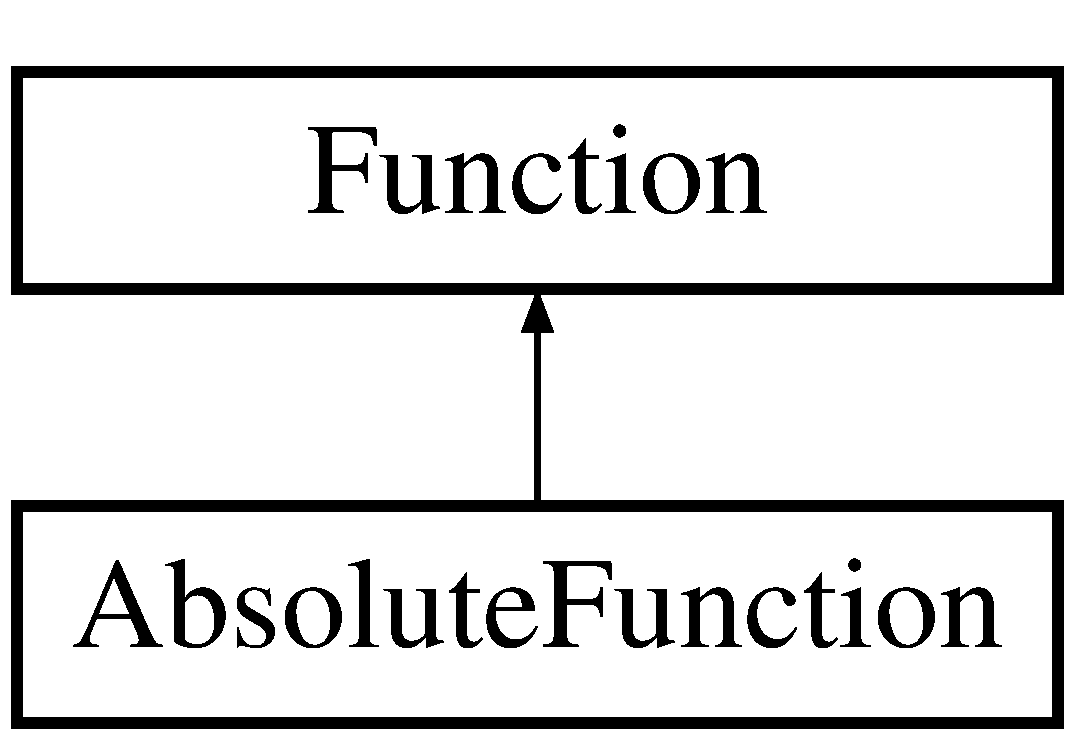
\includegraphics[height=2.000000cm]{class_absolute_function}
\end{center}
\end{figure}
\subsection*{Public Member Functions}
\begin{DoxyCompactItemize}
\item 
virtual Decimal \hyperlink{class_absolute_function_a10fbd656965076a13b6a58ba908b242f}{value\+At} (Decimal x) const 
\begin{DoxyCompactList}\small\item\em Method to determine the value of \hyperlink{class_absolute_function}{Absolute\+Function}. \end{DoxyCompactList}\end{DoxyCompactItemize}


\subsection{Detailed Description}
\hyperlink{class_function}{Function} to compute the absolute value of the input. 

\subsection{Member Function Documentation}
\hypertarget{class_absolute_function_a10fbd656965076a13b6a58ba908b242f}{\index{Absolute\+Function@{Absolute\+Function}!value\+At@{value\+At}}
\index{value\+At@{value\+At}!Absolute\+Function@{Absolute\+Function}}
\subsubsection[{value\+At}]{\setlength{\rightskip}{0pt plus 5cm}virtual Decimal Absolute\+Function\+::value\+At (
\begin{DoxyParamCaption}
\item[{Decimal}]{x}
\end{DoxyParamCaption}
) const\hspace{0.3cm}{\ttfamily [inline]}, {\ttfamily [virtual]}}}\label{class_absolute_function_a10fbd656965076a13b6a58ba908b242f}


Method to determine the value of \hyperlink{class_absolute_function}{Absolute\+Function}. 

\begin{DoxyReturn}{Returns}
The absolute value of {\itshape x}. 
\end{DoxyReturn}


Implements \hyperlink{class_function_a7773feae8f1def0a2d7e479363700816}{Function}.



The documentation for this class was generated from the following file\+:\begin{DoxyCompactItemize}
\item 
Function.\+h\end{DoxyCompactItemize}

\hypertarget{class_canvas}{\section{Canvas Class Reference}
\label{class_canvas}\index{Canvas@{Canvas}}
}


A G\+L window with numerous built-\/in, thread-\/safe drawing operations.  




{\ttfamily \#include $<$Canvas.\+h$>$}

Inheritance diagram for Canvas\+:\begin{figure}[H]
\begin{center}
\leavevmode
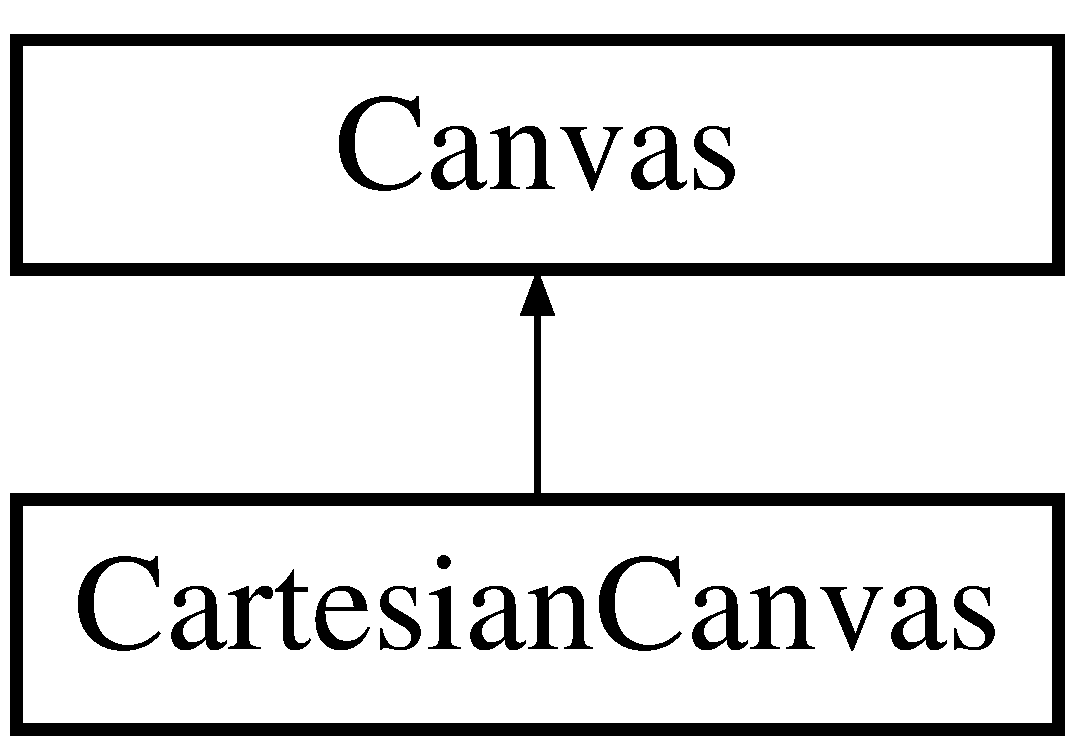
\includegraphics[height=2.000000cm]{class_canvas}
\end{center}
\end{figure}
\subsection*{Public Member Functions}
\begin{DoxyCompactItemize}
\item 
\hyperlink{class_canvas_af80a3103714083bcc2893fbf1f2b72c8}{Canvas} (unsigned int b)
\begin{DoxyCompactList}\small\item\em Constructs a new \hyperlink{class_canvas}{Canvas}. \end{DoxyCompactList}\item 
\hyperlink{class_canvas_a8d81d354d3e6b3229650f2a864750b5b}{Canvas} (int xx, int yy, int w, int h, unsigned int b, std\+::string title=\char`\"{}\char`\"{})
\begin{DoxyCompactList}\small\item\em Explicitly constructs a new \hyperlink{class_canvas}{Canvas}. \end{DoxyCompactList}\item 
\hypertarget{class_canvas_a237c4549ad2e27c729cd1f71e89f0fd9}{virtual \hyperlink{class_canvas_a237c4549ad2e27c729cd1f71e89f0fd9}{$\sim$\+Canvas} ()}\label{class_canvas_a237c4549ad2e27c729cd1f71e89f0fd9}

\begin{DoxyCompactList}\small\item\em Destructor for the \hyperlink{class_canvas}{Canvas} class. \end{DoxyCompactList}\item 
void \hyperlink{class_canvas_a15f16cb84c520e6c4135bfb52434cfae}{bind\+To\+Button} (Key button, Action a, void\+Function f)
\begin{DoxyCompactList}\small\item\em Binds a key or button to a function. \end{DoxyCompactList}\item 
void \hyperlink{class_canvas_a2125433e0574691a9472783694a32bb6}{bind\+To\+Scroll} (std\+::function$<$ void(double, double)$>$ f)
\begin{DoxyCompactList}\small\item\em Binds the mouse wheel to a function. \end{DoxyCompactList}\item 
void \hyperlink{class_canvas_ac4559a6535f497f17415032632aa9f6a}{clear} ()
\begin{DoxyCompactList}\small\item\em Clears the \hyperlink{class_canvas}{Canvas}. \end{DoxyCompactList}\item 
int \hyperlink{class_canvas_aacaad7796cc3519c6cdde08d916bf841}{close} ()
\begin{DoxyCompactList}\small\item\em Waits for the user to close the \hyperlink{class_canvas}{Canvas}. \end{DoxyCompactList}\item 
virtual void \hyperlink{class_canvas_a890f8e6fb35e2dc24cf0892df4981747}{draw\+Circle} (int x, int y, int radius, int res, \hyperlink{struct_color_float}{Color\+Float} color=B\+L\+A\+C\+K, bool filled=true)
\begin{DoxyCompactList}\small\item\em Draw a circle. \end{DoxyCompactList}\item 
virtual void \hyperlink{class_canvas_a867b3202a838e083e5c7bf703d4a3afc}{draw\+Colored\+Polygon} (int size, int x\mbox{[}$\,$\mbox{]}, int y\mbox{[}$\,$\mbox{]}, \hyperlink{struct_color_float}{Color\+Float} color\mbox{[}$\,$\mbox{]}, bool filled=true)
\begin{DoxyCompactList}\small\item\em Draw an arbitrary polygon with colored vertices. \end{DoxyCompactList}\item 
virtual void \hyperlink{class_canvas_a9c9f7c76fa582510c9fd6bac55d013ab}{draw\+Image} (std\+::string fname, int x, int y, int w, int h, float a=1.\+0f)
\begin{DoxyCompactList}\small\item\em Draw an image. \end{DoxyCompactList}\item 
virtual void \hyperlink{class_canvas_a7a017b3bcb4f983b7ea106dea1d1a4f2}{draw\+Line} (int x1, int y1, int x2, int y2, \hyperlink{struct_color_float}{Color\+Float} color=B\+L\+A\+C\+K)
\begin{DoxyCompactList}\small\item\em Draw a line. \end{DoxyCompactList}\item 
virtual void \hyperlink{class_canvas_a6a4cd6d80f90f79e4438deb47b432d74}{draw\+Point} (int x, int y, \hyperlink{struct_color_float}{Color\+Float} color=B\+L\+A\+C\+K)
\begin{DoxyCompactList}\small\item\em Draw a single pixel. \end{DoxyCompactList}\item 
virtual void \hyperlink{class_canvas_a33bb124b99c7621514b2b5220dd0bbc3}{draw\+Rectangle} (int x, int y, int w, int h, \hyperlink{struct_color_float}{Color\+Float} color=B\+L\+A\+C\+K, bool filled=true)
\begin{DoxyCompactList}\small\item\em Draw a rectangle. \end{DoxyCompactList}\item 
virtual void \hyperlink{class_canvas_a751a2e449ec3803934143d5e7cc5cd0a}{draw\+Text} (std\+::wstring s, int x, int y, unsigned int size, \hyperlink{struct_color_float}{Color\+Float} color=B\+L\+A\+C\+K)
\begin{DoxyCompactList}\small\item\em Draw a string of text. \end{DoxyCompactList}\item 
virtual void \hyperlink{class_canvas_a009d8fcfde43d6967cce737778f9e51d}{draw\+Triangle} (int x1, int y1, int x2, int y2, int x3, int y3, \hyperlink{struct_color_float}{Color\+Float} color=B\+L\+A\+C\+K, bool filled=true)
\begin{DoxyCompactList}\small\item\em Draw a triangle. \end{DoxyCompactList}\item 
void \hyperlink{class_canvas_a5118913e1b6d376171b8856ca2f4b508}{end} ()
\begin{DoxyCompactList}\small\item\em Stops the \hyperlink{class_canvas}{Canvas}. \end{DoxyCompactList}\item 
int \hyperlink{class_canvas_a2f17624ba40bc6f98d3675e76c1819d7}{get\+Frame\+Number} ()
\begin{DoxyCompactList}\small\item\em Accessor for the current frame number. \end{DoxyCompactList}\item 
float \hyperlink{class_canvas_a7f5828da2f39dee2602ff624dbe04786}{get\+F\+P\+S} ()
\begin{DoxyCompactList}\small\item\em Accessor for the current F\+P\+S. \end{DoxyCompactList}\item 
bool \hyperlink{class_canvas_ae409ea5d1261a8ad8bb9ef994ffc1c22}{get\+Is\+Open} ()
\begin{DoxyCompactList}\small\item\em Accessor for window's closed status. \end{DoxyCompactList}\item 
int \hyperlink{class_canvas_af5f179835589d447f13544709314c014}{get\+Mouse\+X} ()
\begin{DoxyCompactList}\small\item\em Accessor for the mouse's x-\/position. \end{DoxyCompactList}\item 
int \hyperlink{class_canvas_aad34a217c015181b9457a5c02e8aa8f2}{get\+Mouse\+Y} ()
\begin{DoxyCompactList}\small\item\em Accessor for the mouse's y-\/position. \end{DoxyCompactList}\item 
uint8\+\_\+t $\ast$ \hyperlink{class_canvas_a741d355d9f2021c28e048fc9614e3db2}{get\+Screen\+Buffer} ()
\begin{DoxyCompactList}\small\item\em Accessor for the \hyperlink{class_canvas}{Canvas}'s currently drawn image. \end{DoxyCompactList}\item 
double \hyperlink{class_canvas_a3f212a576d46a0546a86919f4c9fbb57}{get\+Time} ()
\begin{DoxyCompactList}\small\item\em Accessor for the time since the \hyperlink{class_canvas}{Canvas} was initialized. \end{DoxyCompactList}\item 
int \hyperlink{class_canvas_a313206fc26b6f82770ca462f15d0d8c1}{get\+Window\+Width} ()
\begin{DoxyCompactList}\small\item\em Accessor for the \hyperlink{class_canvas}{Canvas}'s width. \end{DoxyCompactList}\item 
int \hyperlink{class_canvas_a59f0970506389b938c2bf1f7c53a3dc5}{get\+Window\+Height} ()
\begin{DoxyCompactList}\small\item\em Accessor for the \hyperlink{class_canvas}{Canvas}'s height. \end{DoxyCompactList}\item 
int \hyperlink{class_canvas_ab3a8868f7261a2a48647ab31000a949b}{get\+Window\+X} ()
\begin{DoxyCompactList}\small\item\em Accessor for the \hyperlink{class_canvas}{Canvas}'s x=position. \end{DoxyCompactList}\item 
int \hyperlink{class_canvas_ad24fcf3335ad5e0761d629aa59d01208}{get\+Window\+Y} ()
\begin{DoxyCompactList}\small\item\em Accessor for the \hyperlink{class_canvas}{Canvas}'s y-\/position. \end{DoxyCompactList}\item 
void \hyperlink{class_canvas_aa298d691c19203544f450cfe0b85cfa0}{record\+For\+Num\+Frames} (unsigned int num\+\_\+frames)
\begin{DoxyCompactList}\small\item\em Records the \hyperlink{class_canvas}{Canvas} for a specified number of frames. \end{DoxyCompactList}\item 
void \hyperlink{class_canvas_a9fa635156cf4e82aa27a7a4878823f1d}{set\+Background\+Color} (\hyperlink{struct_color_float}{Color\+Float} color)
\begin{DoxyCompactList}\small\item\em Mutator for the background color. \end{DoxyCompactList}\item 
void \hyperlink{class_canvas_a72698fe3b651fd6e630884a1ceaadc55}{set\+Font} (std\+::string filename)
\begin{DoxyCompactList}\small\item\em Mutator for the currently loaded font. \end{DoxyCompactList}\item 
void \hyperlink{class_canvas_abb5ef4023451ce81f81112641384e80c}{set\+Show\+F\+P\+S} (bool b)
\begin{DoxyCompactList}\small\item\em Mutator for showing the F\+P\+S. \end{DoxyCompactList}\item 
void \hyperlink{class_canvas_a0a7d72a13049a5af280f2cbc6c49c08d}{set\+Update\+Screen\+Copy} (bool b)
\begin{DoxyCompactList}\small\item\em Mutator for keeping track of the screen's drawn buffer. \end{DoxyCompactList}\item 
void \hyperlink{class_canvas_a6503d6e8efc953a492f04895f5131dff}{stop\+Recording} ()
\begin{DoxyCompactList}\small\item\em Stops recording the \hyperlink{class_canvas}{Canvas}. \end{DoxyCompactList}\item 
int \hyperlink{class_canvas_acb0e91ff615b90fee442ccd43d003a42}{start} ()
\begin{DoxyCompactList}\small\item\em Opens the \hyperlink{class_canvas}{Canvas}. \end{DoxyCompactList}\item 
void \hyperlink{class_canvas_a82f53634a21ab8bf7daf6586ad4c313f}{take\+Screen\+Shot} ()
\begin{DoxyCompactList}\small\item\em Takes a screenshot. \end{DoxyCompactList}\end{DoxyCompactItemize}
\subsection*{Protected Member Functions}
\begin{DoxyCompactItemize}
\item 
\hypertarget{class_canvas_a0165ea279b0438ed67832af40026e21a}{void {\bfseries draw\+Shape} (\hyperlink{class_shape}{Shape} $\ast$s)}\label{class_canvas_a0165ea279b0438ed67832af40026e21a}

\end{DoxyCompactItemize}


\subsection{Detailed Description}
A G\+L window with numerous built-\/in, thread-\/safe drawing operations. 

\hyperlink{class_canvas}{Canvas} provides an easy-\/to-\/set-\/up, easy-\/to-\/use class for drawing various shapes.

With libpng and libjpeg, \hyperlink{class_canvas}{Canvas} also supports the drawing of images.

On top of being easy to use, \hyperlink{class_canvas}{Canvas} is also thread-\/safe, so any number of images may be drawn at once. 

\subsection{Constructor \& Destructor Documentation}
\hypertarget{class_canvas_af80a3103714083bcc2893fbf1f2b72c8}{\index{Canvas@{Canvas}!Canvas@{Canvas}}
\index{Canvas@{Canvas}!Canvas@{Canvas}}
\subsubsection[{Canvas}]{\setlength{\rightskip}{0pt plus 5cm}Canvas\+::\+Canvas (
\begin{DoxyParamCaption}
\item[{unsigned int}]{b}
\end{DoxyParamCaption}
)}}\label{class_canvas_af80a3103714083bcc2893fbf1f2b72c8}


Constructs a new \hyperlink{class_canvas}{Canvas}. 

This is the default constructor for the \hyperlink{class_canvas}{Canvas} class 
\begin{DoxyParams}{Parameters}
{\em b} & The size of the \hyperlink{class_canvas}{Canvas}'s internal vertex buffer. \\
\hline
\end{DoxyParams}
\begin{DoxyReturn}{Returns}
A new 800x600 \hyperlink{class_canvas}{Canvas} in the middle of the screen with no title. 
\end{DoxyReturn}
\hypertarget{class_canvas_a8d81d354d3e6b3229650f2a864750b5b}{\index{Canvas@{Canvas}!Canvas@{Canvas}}
\index{Canvas@{Canvas}!Canvas@{Canvas}}
\subsubsection[{Canvas}]{\setlength{\rightskip}{0pt plus 5cm}Canvas\+::\+Canvas (
\begin{DoxyParamCaption}
\item[{int}]{xx, }
\item[{int}]{yy, }
\item[{int}]{w, }
\item[{int}]{h, }
\item[{unsigned int}]{b, }
\item[{std\+::string}]{title = {\ttfamily \char`\"{}\char`\"{}}}
\end{DoxyParamCaption}
)}}\label{class_canvas_a8d81d354d3e6b3229650f2a864750b5b}


Explicitly constructs a new \hyperlink{class_canvas}{Canvas}. 

This is an explicit constructor for the \hyperlink{class_canvas}{Canvas} class. 
\begin{DoxyParams}{Parameters}
{\em xx} & The x position of the \hyperlink{class_canvas}{Canvas} window. \\
\hline
{\em yy} & The y position of the \hyperlink{class_canvas}{Canvas} window. \\
\hline
{\em w} & The x dimension of the \hyperlink{class_canvas}{Canvas} window. \\
\hline
{\em h} & The y dimension of the \hyperlink{class_canvas}{Canvas} window. \\
\hline
{\em b} & The size of the \hyperlink{class_canvas}{Canvas}'s internal vertex buffer. \\
\hline
{\em title} & The title of the window. \\
\hline
\end{DoxyParams}
\begin{DoxyReturn}{Returns}
A new \hyperlink{class_canvas}{Canvas} with the specified positional data and title. 
\end{DoxyReturn}


\subsection{Member Function Documentation}
\hypertarget{class_canvas_a15f16cb84c520e6c4135bfb52434cfae}{\index{Canvas@{Canvas}!bind\+To\+Button@{bind\+To\+Button}}
\index{bind\+To\+Button@{bind\+To\+Button}!Canvas@{Canvas}}
\subsubsection[{bind\+To\+Button}]{\setlength{\rightskip}{0pt plus 5cm}void Canvas\+::bind\+To\+Button (
\begin{DoxyParamCaption}
\item[{Key}]{button, }
\item[{Action}]{a, }
\item[{void\+Function}]{f}
\end{DoxyParamCaption}
)}}\label{class_canvas_a15f16cb84c520e6c4135bfb52434cfae}


Binds a key or button to a function. 

This function binds a key or mouse button to a function pointer. Upon pressing or releasing the given key, \hyperlink{class_canvas}{Canvas} will call the specified function. 
\begin{DoxyParams}{Parameters}
{\em button} & The key or button to bind, as specified in the Key enum. \\
\hline
{\em a} & The action to look out for (P\+G\+\_\+\+P\+R\+E\+S\+S or P\+G\+\_\+\+R\+E\+L\+E\+A\+S\+E). \\
\hline
{\em f} & The function to call upon action a on button. \\
\hline
\end{DoxyParams}
\begin{DoxyWarning}{Warning}
P\+G\+\_\+\+K\+E\+Y\+\_\+\+E\+S\+C\+A\+P\+E is automatically bound to closing the window. Overriding P\+G\+\_\+\+K\+E\+Y\+\_\+\+E\+S\+C\+A\+P\+E will likely make you unable to close the window. 
\end{DoxyWarning}
\hypertarget{class_canvas_a2125433e0574691a9472783694a32bb6}{\index{Canvas@{Canvas}!bind\+To\+Scroll@{bind\+To\+Scroll}}
\index{bind\+To\+Scroll@{bind\+To\+Scroll}!Canvas@{Canvas}}
\subsubsection[{bind\+To\+Scroll}]{\setlength{\rightskip}{0pt plus 5cm}void Canvas\+::bind\+To\+Scroll (
\begin{DoxyParamCaption}
\item[{std\+::function$<$ void(double, double)$>$}]{f}
\end{DoxyParamCaption}
)}}\label{class_canvas_a2125433e0574691a9472783694a32bb6}


Binds the mouse wheel to a function. 

This function binds the mouse wheel to a function pointer. Upon scrolling, \hyperlink{class_canvas}{Canvas} will call the specified function. 
\begin{DoxyParams}{Parameters}
{\em f} & A function taking x and y parameters to be called when the mouse is scrolled. \\
\hline
\end{DoxyParams}
\hypertarget{class_canvas_ac4559a6535f497f17415032632aa9f6a}{\index{Canvas@{Canvas}!clear@{clear}}
\index{clear@{clear}!Canvas@{Canvas}}
\subsubsection[{clear}]{\setlength{\rightskip}{0pt plus 5cm}void Canvas\+::clear (
\begin{DoxyParamCaption}
{}
\end{DoxyParamCaption}
)}}\label{class_canvas_ac4559a6535f497f17415032632aa9f6a}


Clears the \hyperlink{class_canvas}{Canvas}. 

This function removes all shapes and sets the background to the color specified in \hyperlink{class_canvas_a9fa635156cf4e82aa27a7a4878823f1d}{set\+Background\+Color()}. \hypertarget{class_canvas_aacaad7796cc3519c6cdde08d916bf841}{\index{Canvas@{Canvas}!close@{close}}
\index{close@{close}!Canvas@{Canvas}}
\subsubsection[{close}]{\setlength{\rightskip}{0pt plus 5cm}int Canvas\+::close (
\begin{DoxyParamCaption}
{}
\end{DoxyParamCaption}
)}}\label{class_canvas_aacaad7796cc3519c6cdde08d916bf841}


Waits for the user to close the \hyperlink{class_canvas}{Canvas}. 

This function blocks until the user closes the \hyperlink{class_canvas}{Canvas}. This function has no effect and will not request for close. Use \hyperlink{class_canvas_a5118913e1b6d376171b8856ca2f4b508}{end()} before this to make that request. \begin{DoxyReturn}{Returns}
0 if exit is successful, -\/1 if the canvas has not started yet. 
\end{DoxyReturn}
\begin{DoxySeeAlso}{See also}
\hyperlink{class_canvas_acb0e91ff615b90fee442ccd43d003a42}{start()}, \hyperlink{class_canvas_a5118913e1b6d376171b8856ca2f4b508}{end()} 
\end{DoxySeeAlso}
\hypertarget{class_canvas_a890f8e6fb35e2dc24cf0892df4981747}{\index{Canvas@{Canvas}!draw\+Circle@{draw\+Circle}}
\index{draw\+Circle@{draw\+Circle}!Canvas@{Canvas}}
\subsubsection[{draw\+Circle}]{\setlength{\rightskip}{0pt plus 5cm}void Canvas\+::draw\+Circle (
\begin{DoxyParamCaption}
\item[{int}]{x, }
\item[{int}]{y, }
\item[{int}]{radius, }
\item[{int}]{res, }
\item[{{\bf Color\+Float}}]{color = {\ttfamily BLACK}, }
\item[{bool}]{filled = {\ttfamily true}}
\end{DoxyParamCaption}
)\hspace{0.3cm}{\ttfamily [virtual]}}}\label{class_canvas_a890f8e6fb35e2dc24cf0892df4981747}


Draw a circle. 

This function draws a circle with the given origin coordinates, radius, resolution (number of sides), and color. 
\begin{DoxyParams}{Parameters}
{\em x} & The x coordinate of the circle's origin. \\
\hline
{\em y} & The y coordinate of the circle's origin. \\
\hline
{\em radius} & The radius of the circle in pixels. \\
\hline
{\em res} & The number of sides to use in the circle. \\
\hline
{\em color} & The color of the circle. \\
\hline
{\em filled} & Whether the circle should be filled. \\
\hline
\end{DoxyParams}


Referenced by Cartesian\+Canvas\+::draw\+Circle().

\hypertarget{class_canvas_a867b3202a838e083e5c7bf703d4a3afc}{\index{Canvas@{Canvas}!draw\+Colored\+Polygon@{draw\+Colored\+Polygon}}
\index{draw\+Colored\+Polygon@{draw\+Colored\+Polygon}!Canvas@{Canvas}}
\subsubsection[{draw\+Colored\+Polygon}]{\setlength{\rightskip}{0pt plus 5cm}void Canvas\+::draw\+Colored\+Polygon (
\begin{DoxyParamCaption}
\item[{int}]{size, }
\item[{int}]{x\mbox{[}$\,$\mbox{]}, }
\item[{int}]{y\mbox{[}$\,$\mbox{]}, }
\item[{{\bf Color\+Float}}]{color\mbox{[}$\,$\mbox{]}, }
\item[{bool}]{filled = {\ttfamily true}}
\end{DoxyParamCaption}
)\hspace{0.3cm}{\ttfamily [virtual]}}}\label{class_canvas_a867b3202a838e083e5c7bf703d4a3afc}


Draw an arbitrary polygon with colored vertices. 

This function draws a \hyperlink{class_colored_polygon}{Colored\+Polygon} with the given vertex data 
\begin{DoxyParams}{Parameters}
{\em size} & the number of vertices in the polygon \\
\hline
{\em x} & an array of x positions of the vertices \\
\hline
{\em y} & an array of y positions of the vertices \\
\hline
{\em color} & an array of colors for the vertices \\
\hline
{\em filled} & whether the colored polygon should be filled (true) or not (false) \\
\hline
\end{DoxyParams}


Reimplemented in \hyperlink{class_cartesian_canvas_aa80eb5c58be2461f76a02d0acc94811b}{Cartesian\+Canvas}.



Referenced by Cartesian\+Canvas\+::draw\+Colored\+Polygon().

\hypertarget{class_canvas_a9c9f7c76fa582510c9fd6bac55d013ab}{\index{Canvas@{Canvas}!draw\+Image@{draw\+Image}}
\index{draw\+Image@{draw\+Image}!Canvas@{Canvas}}
\subsubsection[{draw\+Image}]{\setlength{\rightskip}{0pt plus 5cm}void Canvas\+::draw\+Image (
\begin{DoxyParamCaption}
\item[{std\+::string}]{fname, }
\item[{int}]{x, }
\item[{int}]{y, }
\item[{int}]{w, }
\item[{int}]{h, }
\item[{float}]{a = {\ttfamily 1.0f}}
\end{DoxyParamCaption}
)\hspace{0.3cm}{\ttfamily [virtual]}}}\label{class_canvas_a9c9f7c76fa582510c9fd6bac55d013ab}


Draw an image. 

This function draws an \hyperlink{class_image}{Image} with the given coordinates and dimensions. 
\begin{DoxyParams}{Parameters}
{\em fname} & The name of the file to load the image from. \\
\hline
{\em x} & The x coordinate of the \hyperlink{class_image}{Image}'s left edge. \\
\hline
{\em y} & The y coordinate of the \hyperlink{class_image}{Image}'s top edge. \\
\hline
{\em w} & The width of the \hyperlink{class_image}{Image}. \\
\hline
{\em h} & The height of the \hyperlink{class_image}{Image}. \\
\hline
{\em a} & The alpha with which to draw the \hyperlink{class_image}{Image}. \\
\hline
\end{DoxyParams}


Referenced by Cartesian\+Canvas\+::draw\+Image().

\hypertarget{class_canvas_a7a017b3bcb4f983b7ea106dea1d1a4f2}{\index{Canvas@{Canvas}!draw\+Line@{draw\+Line}}
\index{draw\+Line@{draw\+Line}!Canvas@{Canvas}}
\subsubsection[{draw\+Line}]{\setlength{\rightskip}{0pt plus 5cm}void Canvas\+::draw\+Line (
\begin{DoxyParamCaption}
\item[{int}]{x1, }
\item[{int}]{y1, }
\item[{int}]{x2, }
\item[{int}]{y2, }
\item[{{\bf Color\+Float}}]{color = {\ttfamily BLACK}}
\end{DoxyParamCaption}
)\hspace{0.3cm}{\ttfamily [virtual]}}}\label{class_canvas_a7a017b3bcb4f983b7ea106dea1d1a4f2}


Draw a line. 

This function draws a \hyperlink{class_line}{Line} at the given coordinates with the given color. 
\begin{DoxyParams}{Parameters}
{\em x1} & The x position of the start of the line. \\
\hline
{\em y1} & The y position of the start of the line. \\
\hline
{\em x2} & The x position of the end of the line. \\
\hline
{\em y2} & The y position of the end of the line. \\
\hline
{\em color} & The color of the line. \\
\hline
\end{DoxyParams}


Referenced by Cartesian\+Canvas\+::draw\+Line().

\hypertarget{class_canvas_a6a4cd6d80f90f79e4438deb47b432d74}{\index{Canvas@{Canvas}!draw\+Point@{draw\+Point}}
\index{draw\+Point@{draw\+Point}!Canvas@{Canvas}}
\subsubsection[{draw\+Point}]{\setlength{\rightskip}{0pt plus 5cm}void Canvas\+::draw\+Point (
\begin{DoxyParamCaption}
\item[{int}]{x, }
\item[{int}]{y, }
\item[{{\bf Color\+Float}}]{color = {\ttfamily BLACK}}
\end{DoxyParamCaption}
)\hspace{0.3cm}{\ttfamily [virtual]}}}\label{class_canvas_a6a4cd6d80f90f79e4438deb47b432d74}


Draw a single pixel. 

This function draws a Point at the given coordinates with the given color. 
\begin{DoxyParams}{Parameters}
{\em x} & The x position of the point. \\
\hline
{\em y} & The y position of the point. \\
\hline
{\em color} & The color of the point. \\
\hline
\end{DoxyParams}


Referenced by Cartesian\+Canvas\+::draw\+Point().

\hypertarget{class_canvas_a33bb124b99c7621514b2b5220dd0bbc3}{\index{Canvas@{Canvas}!draw\+Rectangle@{draw\+Rectangle}}
\index{draw\+Rectangle@{draw\+Rectangle}!Canvas@{Canvas}}
\subsubsection[{draw\+Rectangle}]{\setlength{\rightskip}{0pt plus 5cm}void Canvas\+::draw\+Rectangle (
\begin{DoxyParamCaption}
\item[{int}]{x, }
\item[{int}]{y, }
\item[{int}]{w, }
\item[{int}]{h, }
\item[{{\bf Color\+Float}}]{color = {\ttfamily BLACK}, }
\item[{bool}]{filled = {\ttfamily true}}
\end{DoxyParamCaption}
)\hspace{0.3cm}{\ttfamily [virtual]}}}\label{class_canvas_a33bb124b99c7621514b2b5220dd0bbc3}


Draw a rectangle. 

This function draws a \hyperlink{class_rectangle}{Rectangle} with the given coordinates, dimensions, and color. 
\begin{DoxyParams}{Parameters}
{\em x} & The x coordinate of the \hyperlink{class_rectangle}{Rectangle}'s left edge. \\
\hline
{\em y} & The y coordinate of the \hyperlink{class_rectangle}{Rectangle}'s top edge. \\
\hline
{\em w} & The width of the \hyperlink{class_rectangle}{Rectangle}. \\
\hline
{\em h} & The height of the \hyperlink{class_rectangle}{Rectangle}. \\
\hline
{\em color} & The color of the rectangle. \\
\hline
{\em filled} & Whether the rectangle should be filled. \\
\hline
\end{DoxyParams}


Referenced by Cartesian\+Canvas\+::draw\+Rectangle().

\hypertarget{class_canvas_a751a2e449ec3803934143d5e7cc5cd0a}{\index{Canvas@{Canvas}!draw\+Text@{draw\+Text}}
\index{draw\+Text@{draw\+Text}!Canvas@{Canvas}}
\subsubsection[{draw\+Text}]{\setlength{\rightskip}{0pt plus 5cm}void Canvas\+::draw\+Text (
\begin{DoxyParamCaption}
\item[{std\+::wstring}]{s, }
\item[{int}]{x, }
\item[{int}]{y, }
\item[{unsigned int}]{size, }
\item[{{\bf Color\+Float}}]{color = {\ttfamily BLACK}}
\end{DoxyParamCaption}
)\hspace{0.3cm}{\ttfamily [virtual]}}}\label{class_canvas_a751a2e449ec3803934143d5e7cc5cd0a}


Draw a string of text. 

This function draws a given string of \hyperlink{class_text}{Text} at the given coordinates with the given color. 
\begin{DoxyParams}{Parameters}
{\em s} & The string to draw. \\
\hline
{\em x} & The x coordinate of the text's left bound. \\
\hline
{\em y} & The y coordinate of the text's left bound. \\
\hline
{\em size} & The size of the text in pixels. \\
\hline
{\em color} & The color of the \hyperlink{class_text}{Text}. \\
\hline
\end{DoxyParams}


Referenced by Cartesian\+Canvas\+::draw\+Text().

\hypertarget{class_canvas_a009d8fcfde43d6967cce737778f9e51d}{\index{Canvas@{Canvas}!draw\+Triangle@{draw\+Triangle}}
\index{draw\+Triangle@{draw\+Triangle}!Canvas@{Canvas}}
\subsubsection[{draw\+Triangle}]{\setlength{\rightskip}{0pt plus 5cm}void Canvas\+::draw\+Triangle (
\begin{DoxyParamCaption}
\item[{int}]{x1, }
\item[{int}]{y1, }
\item[{int}]{x2, }
\item[{int}]{y2, }
\item[{int}]{x3, }
\item[{int}]{y3, }
\item[{{\bf Color\+Float}}]{color = {\ttfamily BLACK}, }
\item[{bool}]{filled = {\ttfamily true}}
\end{DoxyParamCaption}
)\hspace{0.3cm}{\ttfamily [virtual]}}}\label{class_canvas_a009d8fcfde43d6967cce737778f9e51d}


Draw a triangle. 

This function draws a \hyperlink{class_triangle}{Triangle} with the given vertices. 
\begin{DoxyParams}{Parameters}
{\em x1} & the x coordinate of the first vertex of the \hyperlink{class_triangle}{Triangle}. \\
\hline
{\em y1} & the y coordinate of the first vertex of the \hyperlink{class_triangle}{Triangle}. \\
\hline
{\em x2} & the x coordinate of the second vertex of the \hyperlink{class_triangle}{Triangle}. \\
\hline
{\em y2} & the y coordinate of the second vertex of the \hyperlink{class_triangle}{Triangle}. \\
\hline
{\em x3} & the x coordinate of the third vertex of the \hyperlink{class_triangle}{Triangle}. \\
\hline
{\em y3} & the y coordinate of the third vertex of the \hyperlink{class_triangle}{Triangle}. \\
\hline
{\em color} & the color of the \hyperlink{class_triangle}{Triangle}. \\
\hline
{\em filled} & Whether the \hyperlink{class_triangle}{Triangle} should be filled. \\
\hline
\end{DoxyParams}


Referenced by Cartesian\+Canvas\+::draw\+Triangle().

\hypertarget{class_canvas_a5118913e1b6d376171b8856ca2f4b508}{\index{Canvas@{Canvas}!end@{end}}
\index{end@{end}!Canvas@{Canvas}}
\subsubsection[{end}]{\setlength{\rightskip}{0pt plus 5cm}void Canvas\+::end (
\begin{DoxyParamCaption}
{}
\end{DoxyParamCaption}
)}}\label{class_canvas_a5118913e1b6d376171b8856ca2f4b508}


Stops the \hyperlink{class_canvas}{Canvas}. 

This function stops rendering the \hyperlink{class_canvas}{Canvas}. This does not close the \hyperlink{class_canvas}{Canvas}; it will stay open. To rejoin the threads and complete the close, \hyperlink{class_canvas_aacaad7796cc3519c6cdde08d916bf841}{close()} must be called. \hyperlink{class_canvas_a5118913e1b6d376171b8856ca2f4b508}{end()} is not required to close the \hyperlink{class_canvas}{Canvas}, closing the window by hitting escape or with the window manager does the same thing.

Once \hyperlink{class_canvas_a5118913e1b6d376171b8856ca2f4b508}{end()} has been called, either manually, by the window manager, or by pressing escape, \hyperlink{class_canvas_ae409ea5d1261a8ad8bb9ef994ffc1c22}{get\+Is\+Open()} will return false, and your computation should exit. \begin{DoxySeeAlso}{See also}
\hyperlink{class_canvas_acb0e91ff615b90fee442ccd43d003a42}{start()}, \hyperlink{class_canvas_aacaad7796cc3519c6cdde08d916bf841}{close()} 
\end{DoxySeeAlso}
\hypertarget{class_canvas_a7f5828da2f39dee2602ff624dbe04786}{\index{Canvas@{Canvas}!get\+F\+P\+S@{get\+F\+P\+S}}
\index{get\+F\+P\+S@{get\+F\+P\+S}!Canvas@{Canvas}}
\subsubsection[{get\+F\+P\+S}]{\setlength{\rightskip}{0pt plus 5cm}float Canvas\+::get\+F\+P\+S (
\begin{DoxyParamCaption}
{}
\end{DoxyParamCaption}
)}}\label{class_canvas_a7f5828da2f39dee2602ff624dbe04786}


Accessor for the current F\+P\+S. 

\begin{DoxyReturn}{Returns}
The current actual F\+P\+S. 
\end{DoxyReturn}
\hypertarget{class_canvas_a2f17624ba40bc6f98d3675e76c1819d7}{\index{Canvas@{Canvas}!get\+Frame\+Number@{get\+Frame\+Number}}
\index{get\+Frame\+Number@{get\+Frame\+Number}!Canvas@{Canvas}}
\subsubsection[{get\+Frame\+Number}]{\setlength{\rightskip}{0pt plus 5cm}int Canvas\+::get\+Frame\+Number (
\begin{DoxyParamCaption}
{}
\end{DoxyParamCaption}
)}}\label{class_canvas_a2f17624ba40bc6f98d3675e76c1819d7}


Accessor for the current frame number. 

\begin{DoxyReturn}{Returns}
The number of frames rendered so far. 
\end{DoxyReturn}
\hypertarget{class_canvas_ae409ea5d1261a8ad8bb9ef994ffc1c22}{\index{Canvas@{Canvas}!get\+Is\+Open@{get\+Is\+Open}}
\index{get\+Is\+Open@{get\+Is\+Open}!Canvas@{Canvas}}
\subsubsection[{get\+Is\+Open}]{\setlength{\rightskip}{0pt plus 5cm}bool Canvas\+::get\+Is\+Open (
\begin{DoxyParamCaption}
{}
\end{DoxyParamCaption}
)}}\label{class_canvas_ae409ea5d1261a8ad8bb9ef994ffc1c22}


Accessor for window's closed status. 

\begin{DoxyReturn}{Returns}
Whether the window is still open (that is, the user has not closed it). 
\end{DoxyReturn}
\hypertarget{class_canvas_af5f179835589d447f13544709314c014}{\index{Canvas@{Canvas}!get\+Mouse\+X@{get\+Mouse\+X}}
\index{get\+Mouse\+X@{get\+Mouse\+X}!Canvas@{Canvas}}
\subsubsection[{get\+Mouse\+X}]{\setlength{\rightskip}{0pt plus 5cm}int Canvas\+::get\+Mouse\+X (
\begin{DoxyParamCaption}
{}
\end{DoxyParamCaption}
)}}\label{class_canvas_af5f179835589d447f13544709314c014}


Accessor for the mouse's x-\/position. 

\begin{DoxyReturn}{Returns}
The x coordinates of the mouse on the \hyperlink{class_canvas}{Canvas}. 
\end{DoxyReturn}
\hypertarget{class_canvas_aad34a217c015181b9457a5c02e8aa8f2}{\index{Canvas@{Canvas}!get\+Mouse\+Y@{get\+Mouse\+Y}}
\index{get\+Mouse\+Y@{get\+Mouse\+Y}!Canvas@{Canvas}}
\subsubsection[{get\+Mouse\+Y}]{\setlength{\rightskip}{0pt plus 5cm}int Canvas\+::get\+Mouse\+Y (
\begin{DoxyParamCaption}
{}
\end{DoxyParamCaption}
)}}\label{class_canvas_aad34a217c015181b9457a5c02e8aa8f2}


Accessor for the mouse's y-\/position. 

\begin{DoxyReturn}{Returns}
The y coordinates of the mouse on the \hyperlink{class_canvas}{Canvas}. 
\end{DoxyReturn}
\hypertarget{class_canvas_a741d355d9f2021c28e048fc9614e3db2}{\index{Canvas@{Canvas}!get\+Screen\+Buffer@{get\+Screen\+Buffer}}
\index{get\+Screen\+Buffer@{get\+Screen\+Buffer}!Canvas@{Canvas}}
\subsubsection[{get\+Screen\+Buffer}]{\setlength{\rightskip}{0pt plus 5cm}uint8\+\_\+t $\ast$ Canvas\+::get\+Screen\+Buffer (
\begin{DoxyParamCaption}
{}
\end{DoxyParamCaption}
)}}\label{class_canvas_a741d355d9f2021c28e048fc9614e3db2}


Accessor for the \hyperlink{class_canvas}{Canvas}'s currently drawn image. 

\begin{DoxyReturn}{Returns}
A pointer to the R\+G\+B pixel buffer for the current \hyperlink{class_canvas}{Canvas}. 
\end{DoxyReturn}
\hypertarget{class_canvas_a3f212a576d46a0546a86919f4c9fbb57}{\index{Canvas@{Canvas}!get\+Time@{get\+Time}}
\index{get\+Time@{get\+Time}!Canvas@{Canvas}}
\subsubsection[{get\+Time}]{\setlength{\rightskip}{0pt plus 5cm}double Canvas\+::get\+Time (
\begin{DoxyParamCaption}
{}
\end{DoxyParamCaption}
)}}\label{class_canvas_a3f212a576d46a0546a86919f4c9fbb57}


Accessor for the time since the \hyperlink{class_canvas}{Canvas} was initialized. 

\begin{DoxyReturn}{Returns}
The time elapsed since the \hyperlink{class_canvas}{Canvas} has started drawing (in microseconds). 
\end{DoxyReturn}
\hypertarget{class_canvas_a59f0970506389b938c2bf1f7c53a3dc5}{\index{Canvas@{Canvas}!get\+Window\+Height@{get\+Window\+Height}}
\index{get\+Window\+Height@{get\+Window\+Height}!Canvas@{Canvas}}
\subsubsection[{get\+Window\+Height}]{\setlength{\rightskip}{0pt plus 5cm}int Canvas\+::get\+Window\+Height (
\begin{DoxyParamCaption}
{}
\end{DoxyParamCaption}
)}}\label{class_canvas_a59f0970506389b938c2bf1f7c53a3dc5}


Accessor for the \hyperlink{class_canvas}{Canvas}'s height. 

\begin{DoxyReturn}{Returns}
The height in pixels of the \hyperlink{class_canvas}{Canvas}. 
\end{DoxyReturn}


Referenced by Cartesian\+Canvas\+::get\+Cartesian\+Coordinates(), Cartesian\+Canvas\+::get\+Screen\+Coordinates(), and Cartesian\+Canvas\+::recompute\+Dimensions().

\hypertarget{class_canvas_a313206fc26b6f82770ca462f15d0d8c1}{\index{Canvas@{Canvas}!get\+Window\+Width@{get\+Window\+Width}}
\index{get\+Window\+Width@{get\+Window\+Width}!Canvas@{Canvas}}
\subsubsection[{get\+Window\+Width}]{\setlength{\rightskip}{0pt plus 5cm}int Canvas\+::get\+Window\+Width (
\begin{DoxyParamCaption}
{}
\end{DoxyParamCaption}
)}}\label{class_canvas_a313206fc26b6f82770ca462f15d0d8c1}


Accessor for the \hyperlink{class_canvas}{Canvas}'s width. 

\begin{DoxyReturn}{Returns}
The width in pixels of the \hyperlink{class_canvas}{Canvas}. 
\end{DoxyReturn}


Referenced by Cartesian\+Canvas\+::get\+Cartesian\+Coordinates(), Cartesian\+Canvas\+::get\+Screen\+Coordinates(), and Cartesian\+Canvas\+::recompute\+Dimensions().

\hypertarget{class_canvas_ab3a8868f7261a2a48647ab31000a949b}{\index{Canvas@{Canvas}!get\+Window\+X@{get\+Window\+X}}
\index{get\+Window\+X@{get\+Window\+X}!Canvas@{Canvas}}
\subsubsection[{get\+Window\+X}]{\setlength{\rightskip}{0pt plus 5cm}int Canvas\+::get\+Window\+X (
\begin{DoxyParamCaption}
{}
\end{DoxyParamCaption}
)}}\label{class_canvas_ab3a8868f7261a2a48647ab31000a949b}


Accessor for the \hyperlink{class_canvas}{Canvas}'s x=position. 

\begin{DoxyReturn}{Returns}
The x coordinate in pixels of the \hyperlink{class_canvas}{Canvas} (0 = left of monitor). 
\end{DoxyReturn}
\hypertarget{class_canvas_ad24fcf3335ad5e0761d629aa59d01208}{\index{Canvas@{Canvas}!get\+Window\+Y@{get\+Window\+Y}}
\index{get\+Window\+Y@{get\+Window\+Y}!Canvas@{Canvas}}
\subsubsection[{get\+Window\+Y}]{\setlength{\rightskip}{0pt plus 5cm}int Canvas\+::get\+Window\+Y (
\begin{DoxyParamCaption}
{}
\end{DoxyParamCaption}
)}}\label{class_canvas_ad24fcf3335ad5e0761d629aa59d01208}


Accessor for the \hyperlink{class_canvas}{Canvas}'s y-\/position. 

\begin{DoxyReturn}{Returns}
The y coordinate in pixels of the \hyperlink{class_canvas}{Canvas} (0 = top of monitor). 
\end{DoxyReturn}
\hypertarget{class_canvas_aa298d691c19203544f450cfe0b85cfa0}{\index{Canvas@{Canvas}!record\+For\+Num\+Frames@{record\+For\+Num\+Frames}}
\index{record\+For\+Num\+Frames@{record\+For\+Num\+Frames}!Canvas@{Canvas}}
\subsubsection[{record\+For\+Num\+Frames}]{\setlength{\rightskip}{0pt plus 5cm}void Canvas\+::record\+For\+Num\+Frames (
\begin{DoxyParamCaption}
\item[{unsigned int}]{num\+\_\+frames}
\end{DoxyParamCaption}
)}}\label{class_canvas_aa298d691c19203544f450cfe0b85cfa0}


Records the \hyperlink{class_canvas}{Canvas} for a specified number of frames. 

This function starts dumping screenshots of the \hyperlink{class_canvas}{Canvas} to the file system every draw cycle. The function automatically terminates after num\+\_\+frames cycles have completed. \hypertarget{class_canvas_a9fa635156cf4e82aa27a7a4878823f1d}{\index{Canvas@{Canvas}!set\+Background\+Color@{set\+Background\+Color}}
\index{set\+Background\+Color@{set\+Background\+Color}!Canvas@{Canvas}}
\subsubsection[{set\+Background\+Color}]{\setlength{\rightskip}{0pt plus 5cm}void Canvas\+::set\+Background\+Color (
\begin{DoxyParamCaption}
\item[{{\bf Color\+Float}}]{color}
\end{DoxyParamCaption}
)}}\label{class_canvas_a9fa635156cf4e82aa27a7a4878823f1d}


Mutator for the background color. 

This function sets the color to clear to when \hyperlink{class_canvas_ac4559a6535f497f17415032632aa9f6a}{Canvas\+::clear()} is called. 
\begin{DoxyParams}{Parameters}
{\em color} & The color to clear to. \\
\hline
\end{DoxyParams}
\begin{DoxyNote}{Note}
The alpha channel of the color is ignored 
\end{DoxyNote}
\hypertarget{class_canvas_a72698fe3b651fd6e630884a1ceaadc55}{\index{Canvas@{Canvas}!set\+Font@{set\+Font}}
\index{set\+Font@{set\+Font}!Canvas@{Canvas}}
\subsubsection[{set\+Font}]{\setlength{\rightskip}{0pt plus 5cm}void Canvas\+::set\+Font (
\begin{DoxyParamCaption}
\item[{std\+::string}]{filename}
\end{DoxyParamCaption}
)}}\label{class_canvas_a72698fe3b651fd6e630884a1ceaadc55}


Mutator for the currently loaded font. 

This function sets the loaded font, loading from the file or from disk if the file was loaded previously. Subsequent calls to \hyperlink{class_canvas_a751a2e449ec3803934143d5e7cc5cd0a}{draw\+Text()} will use this font to print. 
\begin{DoxyParams}{Parameters}
{\em filename} & The filename of the font to load. \\
\hline
\end{DoxyParams}
\begin{DoxyNote}{Note}
Supports all font types that Free\+Type supports, which is almost anything. 
\end{DoxyNote}
\hypertarget{class_canvas_abb5ef4023451ce81f81112641384e80c}{\index{Canvas@{Canvas}!set\+Show\+F\+P\+S@{set\+Show\+F\+P\+S}}
\index{set\+Show\+F\+P\+S@{set\+Show\+F\+P\+S}!Canvas@{Canvas}}
\subsubsection[{set\+Show\+F\+P\+S}]{\setlength{\rightskip}{0pt plus 5cm}void Canvas\+::set\+Show\+F\+P\+S (
\begin{DoxyParamCaption}
\item[{bool}]{b}
\end{DoxyParamCaption}
)}}\label{class_canvas_abb5ef4023451ce81f81112641384e80c}


Mutator for showing the F\+P\+S. 


\begin{DoxyParams}{Parameters}
{\em b} & Whether to print the F\+P\+S to stdout every draw cycle (for debugging purposes). \\
\hline
\end{DoxyParams}
\hypertarget{class_canvas_a0a7d72a13049a5af280f2cbc6c49c08d}{\index{Canvas@{Canvas}!set\+Update\+Screen\+Copy@{set\+Update\+Screen\+Copy}}
\index{set\+Update\+Screen\+Copy@{set\+Update\+Screen\+Copy}!Canvas@{Canvas}}
\subsubsection[{set\+Update\+Screen\+Copy}]{\setlength{\rightskip}{0pt plus 5cm}void Canvas\+::set\+Update\+Screen\+Copy (
\begin{DoxyParamCaption}
\item[{bool}]{b}
\end{DoxyParamCaption}
)}}\label{class_canvas_a0a7d72a13049a5af280f2cbc6c49c08d}


Mutator for keeping track of the screen's drawn buffer. 


\begin{DoxyParams}{Parameters}
{\em b} & Whether to copy the screen's contents to an R\+G\+B color buffer every draw cycle. \\
\hline
\end{DoxyParams}
\begin{DoxyNote}{Note}
The buffer in question can be accessed with \hyperlink{class_canvas_a741d355d9f2021c28e048fc9614e3db2}{get\+Screen\+Buffer()}. 

\hyperlink{class_canvas_a82f53634a21ab8bf7daf6586ad4c313f}{take\+Screen\+Shot()} and \hyperlink{class_canvas_aa298d691c19203544f450cfe0b85cfa0}{record\+For\+Num\+Frames()} automatically sets this to true. 
\end{DoxyNote}
\hypertarget{class_canvas_acb0e91ff615b90fee442ccd43d003a42}{\index{Canvas@{Canvas}!start@{start}}
\index{start@{start}!Canvas@{Canvas}}
\subsubsection[{start}]{\setlength{\rightskip}{0pt plus 5cm}int Canvas\+::start (
\begin{DoxyParamCaption}
{}
\end{DoxyParamCaption}
)}}\label{class_canvas_acb0e91ff615b90fee442ccd43d003a42}


Opens the \hyperlink{class_canvas}{Canvas}. 

This function starts rendering the \hyperlink{class_canvas}{Canvas}. \begin{DoxyReturn}{Returns}
0 if start is successful, -\/1 if the canvas has already started. 
\end{DoxyReturn}
\begin{DoxySeeAlso}{See also}
\hyperlink{class_canvas_aacaad7796cc3519c6cdde08d916bf841}{close()}, \hyperlink{class_canvas_a5118913e1b6d376171b8856ca2f4b508}{end()} 
\end{DoxySeeAlso}
\hypertarget{class_canvas_a6503d6e8efc953a492f04895f5131dff}{\index{Canvas@{Canvas}!stop\+Recording@{stop\+Recording}}
\index{stop\+Recording@{stop\+Recording}!Canvas@{Canvas}}
\subsubsection[{stop\+Recording}]{\setlength{\rightskip}{0pt plus 5cm}void Canvas\+::stop\+Recording (
\begin{DoxyParamCaption}
{}
\end{DoxyParamCaption}
)}}\label{class_canvas_a6503d6e8efc953a492f04895f5131dff}


Stops recording the \hyperlink{class_canvas}{Canvas}. 

This function stops dumping images to the file system. \hypertarget{class_canvas_a82f53634a21ab8bf7daf6586ad4c313f}{\index{Canvas@{Canvas}!take\+Screen\+Shot@{take\+Screen\+Shot}}
\index{take\+Screen\+Shot@{take\+Screen\+Shot}!Canvas@{Canvas}}
\subsubsection[{take\+Screen\+Shot}]{\setlength{\rightskip}{0pt plus 5cm}void Canvas\+::take\+Screen\+Shot (
\begin{DoxyParamCaption}
{}
\end{DoxyParamCaption}
)}}\label{class_canvas_a82f53634a21ab8bf7daf6586ad4c313f}


Takes a screenshot. 

This function saves a screenshot of the current \hyperlink{class_canvas}{Canvas} to the working directory. \begin{DoxyRefDesc}{Bug}
\item[\hyperlink{bug__bug000001}{Bug}]Multiple calls to this function in rapid succession seem to make the F\+P\+S counter inaccurate and make rendering slowdown. \end{DoxyRefDesc}


The documentation for this class was generated from the following files\+:\begin{DoxyCompactItemize}
\item 
Canvas.\+h\item 
Canvas.\+cpp\end{DoxyCompactItemize}

\hypertarget{class_cartesian_canvas}{\section{Cartesian\+Canvas Class Reference}
\label{class_cartesian_canvas}\index{Cartesian\+Canvas@{Cartesian\+Canvas}}
}


\hyperlink{class_canvas}{Canvas} extended for graphic support.  




{\ttfamily \#include $<$Cartesian\+Canvas.\+h$>$}

Inheritance diagram for Cartesian\+Canvas\+:\begin{figure}[H]
\begin{center}
\leavevmode
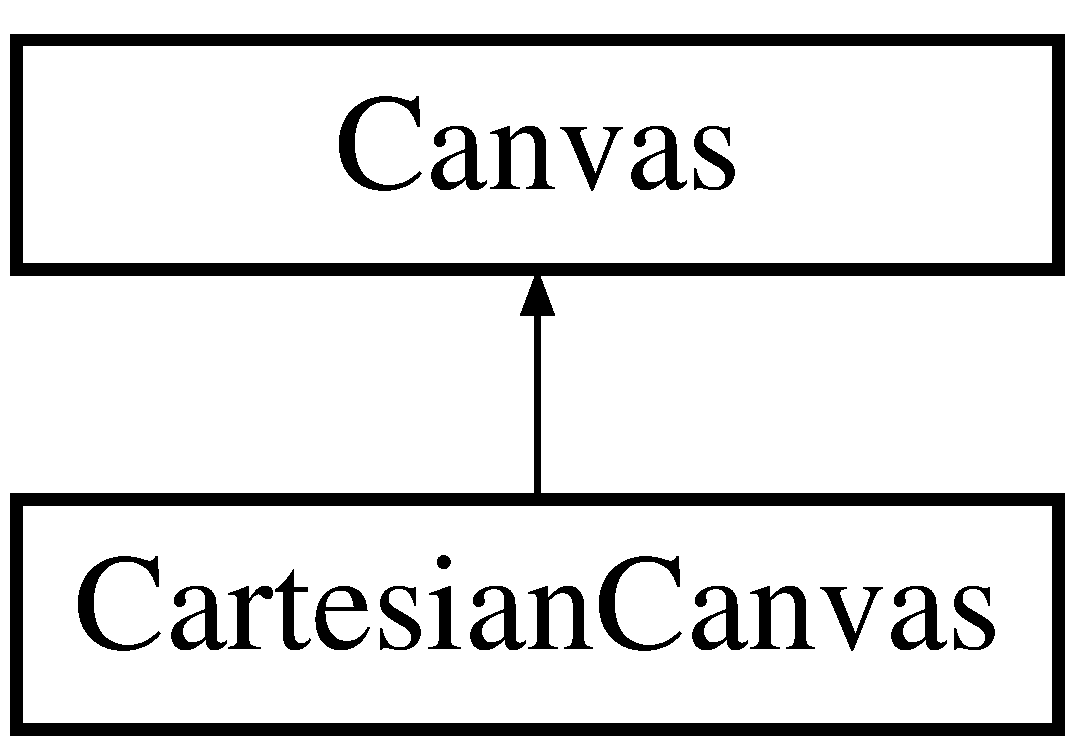
\includegraphics[height=2.000000cm]{class_cartesian_canvas}
\end{center}
\end{figure}
\subsection*{Public Member Functions}
\begin{DoxyCompactItemize}
\item 
\hyperlink{class_cartesian_canvas_ab4387f0226721981adf82ee150751ce0}{Cartesian\+Canvas} (unsigned int b)
\begin{DoxyCompactList}\small\item\em Constructs a new \hyperlink{class_cartesian_canvas}{Cartesian\+Canvas}. \end{DoxyCompactList}\item 
\hyperlink{class_cartesian_canvas_ad9a52e5b74df4f6910eb3a2bbac190bf}{Cartesian\+Canvas} (int xx, int yy, int w, int h, Decimal x\+Min, Decimal y\+Min, Decimal x\+Max, Decimal y\+Max, unsigned int b, std\+::string=\char`\"{}\char`\"{})
\begin{DoxyCompactList}\small\item\em Explicitly constructs a new \hyperlink{class_cartesian_canvas}{Cartesian\+Canvas}. \end{DoxyCompactList}\item 
void \hyperlink{class_cartesian_canvas_a24ff3802f7f82e6f8b89993346e50408}{draw\+Axes} (Decimal x, Decimal y, Decimal dx, Decimal dy)
\begin{DoxyCompactList}\small\item\em Draw axes. \end{DoxyCompactList}\item 
void \hyperlink{class_cartesian_canvas_a9acc954ccb5a9df491db2e8481b58b03}{draw\+Circle} (Decimal x, Decimal y, Decimal radius, int res, \hyperlink{struct_color_float}{Color\+Float} color=B\+L\+A\+C\+K, bool filled=true)
\begin{DoxyCompactList}\small\item\em Draw a circle. \end{DoxyCompactList}\item 
void \hyperlink{class_cartesian_canvas_aa80eb5c58be2461f76a02d0acc94811b}{draw\+Colored\+Polygon} (int size, int x\mbox{[}$\,$\mbox{]}, int y\mbox{[}$\,$\mbox{]}, \hyperlink{struct_color_float}{Color\+Float} color\mbox{[}$\,$\mbox{]}, bool filled=true)
\begin{DoxyCompactList}\small\item\em Draw an arbitrary polygon with colored vertices. \end{DoxyCompactList}\item 
void \hyperlink{class_cartesian_canvas_abfa7f10eb248cf6f4bf7400715ec13ac}{draw\+Function} (const \hyperlink{class_function}{Function} \&f)
\begin{DoxyCompactList}\small\item\em Plots a function on the screen. \end{DoxyCompactList}\item 
void \hyperlink{class_cartesian_canvas_a005e388fa00cc3cc7549f657cd58db84}{draw\+Image} (std\+::string fname, Decimal x, Decimal y, Decimal w, Decimal h, float a=1.\+0f)
\begin{DoxyCompactList}\small\item\em Draw an image. \end{DoxyCompactList}\item 
void \hyperlink{class_cartesian_canvas_a364a55de8ac9d0734a44a4b4af9d5af5}{draw\+Line} (Decimal x1, Decimal y1, Decimal x2, Decimal y2, \hyperlink{struct_color_float}{Color\+Float} color=B\+L\+A\+C\+K)
\begin{DoxyCompactList}\small\item\em Draw a line. \end{DoxyCompactList}\item 
void \hyperlink{class_cartesian_canvas_aa8d3c41d0b54358245b0164230225f05}{draw\+Point} (Decimal x, Decimal y, \hyperlink{struct_color_float}{Color\+Float} color=B\+L\+A\+C\+K)
\begin{DoxyCompactList}\small\item\em Draw a single pixel. \end{DoxyCompactList}\item 
void \hyperlink{class_cartesian_canvas_a54ad4dd438a1cbb1353fb3cb5c5da5c4}{draw\+Rectangle} (Decimal x, Decimal y, Decimal w, Decimal h, \hyperlink{struct_color_float}{Color\+Float} color=B\+L\+A\+C\+K, bool filled=true)
\begin{DoxyCompactList}\small\item\em Draw a rectangle. \end{DoxyCompactList}\item 
void \hyperlink{class_cartesian_canvas_a27f832df7e100315a8ceb385e133326f}{draw\+Text} (std\+::wstring s, Decimal x, Decimal y, unsigned int size, \hyperlink{struct_color_float}{Color\+Float} color=B\+L\+A\+C\+K)
\begin{DoxyCompactList}\small\item\em Draw a string of text. \end{DoxyCompactList}\item 
void \hyperlink{class_cartesian_canvas_a72ddd5a50452068da422fa36847de378}{draw\+Triangle} (Decimal x1, Decimal y1, Decimal x2, Decimal y2, Decimal x3, Decimal y3, \hyperlink{struct_color_float}{Color\+Float} color=B\+L\+A\+C\+K, bool filled=true)
\begin{DoxyCompactList}\small\item\em Draw a triangle. \end{DoxyCompactList}\item 
void \hyperlink{class_cartesian_canvas_a022ac6bdb68f70b9d0dca1edc0f6cc05}{get\+Cartesian\+Coordinates} (int screen\+X, int screen\+Y, Decimal \&cart\+X, Decimal \&cart\+Y)
\begin{DoxyCompactList}\small\item\em Translates Cartesian coordinates into window coordinates. \end{DoxyCompactList}\item 
Decimal \hyperlink{class_cartesian_canvas_a00ab6f569e805c9ee662b1dba3f90b90}{get\+Cart\+Height} ()
\begin{DoxyCompactList}\small\item\em Accessor for the \hyperlink{class_cartesian_canvas}{Cartesian\+Canvas}'s Cartesian height. \end{DoxyCompactList}\item 
Decimal \hyperlink{class_cartesian_canvas_a2a89763ee9a724fb1b07b3fc7c7351a2}{get\+Cart\+Width} ()
\begin{DoxyCompactList}\small\item\em Accessor for the \hyperlink{class_cartesian_canvas}{Cartesian\+Canvas}'s Cartesian width. \end{DoxyCompactList}\item 
Decimal \hyperlink{class_cartesian_canvas_a07fffa1ea919da9022e23aaa25a175d8}{get\+Pixel\+Width} ()
\begin{DoxyCompactList}\small\item\em Accessor for the \hyperlink{class_cartesian_canvas}{Cartesian\+Canvas}'s effective pixel width. \end{DoxyCompactList}\item 
Decimal \hyperlink{class_cartesian_canvas_a9acb1906f1423f336654be45ee7b2a82}{get\+Pixel\+Height} ()
\begin{DoxyCompactList}\small\item\em Accessor for the \hyperlink{class_cartesian_canvas}{Cartesian\+Canvas}'s effective pixel height. \end{DoxyCompactList}\item 
Decimal \hyperlink{class_cartesian_canvas_a494303f706ba4170b7e4ff011b9eab5e}{get\+Max\+X} ()
\begin{DoxyCompactList}\small\item\em Accessor for the \hyperlink{class_cartesian_canvas}{Cartesian\+Canvas}'s right bound. \end{DoxyCompactList}\item 
Decimal \hyperlink{class_cartesian_canvas_a84b1a32b3af487cea0588bd6f09a246e}{get\+Max\+Y} ()
\begin{DoxyCompactList}\small\item\em Accessor for the \hyperlink{class_cartesian_canvas}{Cartesian\+Canvas}'s top bound. \end{DoxyCompactList}\item 
Decimal \hyperlink{class_cartesian_canvas_a598f84f3fda5bea7df9a90952c60ee2c}{get\+Min\+X} ()
\begin{DoxyCompactList}\small\item\em Accessor for the \hyperlink{class_cartesian_canvas}{Cartesian\+Canvas}'s left bound. \end{DoxyCompactList}\item 
Decimal \hyperlink{class_cartesian_canvas_a970a5877d36bc958564556cae1c3c1cb}{get\+Min\+Y} ()
\begin{DoxyCompactList}\small\item\em Accessor for the \hyperlink{class_cartesian_canvas}{Cartesian\+Canvas}'s bottom bound. \end{DoxyCompactList}\item 
void \hyperlink{class_cartesian_canvas_abfe025d3658afe6cf30057e4db7bbc19}{get\+Screen\+Coordinates} (Decimal cart\+X, Decimal cart\+Y, int \&screen\+X, int \&screen\+Y)
\begin{DoxyCompactList}\small\item\em Translates window coordinates into Cartesian coordinates. \end{DoxyCompactList}\item 
void \hyperlink{class_cartesian_canvas_a390eb6c87ec9974bc0c9930e8a8d40ac}{recompute\+Dimensions} (Decimal x\+Min, Decimal y\+Min, Decimal x\+Max, Decimal y\+Max)
\begin{DoxyCompactList}\small\item\em Recomputes the \hyperlink{class_cartesian_canvas}{Cartesian\+Canvas}'s bounds. \end{DoxyCompactList}\item 
void \hyperlink{class_cartesian_canvas_adffe30c84884e8046ebb30438ee8eef1}{zoom} (Decimal x, Decimal y, Decimal scale)
\begin{DoxyCompactList}\small\item\em Zoom the \hyperlink{class_cartesian_canvas}{Cartesian\+Canvas} with a given center. \end{DoxyCompactList}\item 
void \hyperlink{class_cartesian_canvas_a048f37a8e92d248edad546d470432f3c}{zoom} (Decimal x1, Decimal y1, Decimal x2, Decimal y2)
\begin{DoxyCompactList}\small\item\em Zoom the \hyperlink{class_cartesian_canvas}{Cartesian\+Canvas} with the given bounding (Cartesian) coordinates. \end{DoxyCompactList}\end{DoxyCompactItemize}
\subsection*{Additional Inherited Members}


\subsection{Detailed Description}
\hyperlink{class_canvas}{Canvas} extended for graphic support. 

\hyperlink{class_cartesian_canvas}{Cartesian\+Canvas} provides a \hyperlink{class_canvas}{Canvas} with a Cartesian coordinate system for ease of plotting. 

\subsection{Constructor \& Destructor Documentation}
\hypertarget{class_cartesian_canvas_ab4387f0226721981adf82ee150751ce0}{\index{Cartesian\+Canvas@{Cartesian\+Canvas}!Cartesian\+Canvas@{Cartesian\+Canvas}}
\index{Cartesian\+Canvas@{Cartesian\+Canvas}!Cartesian\+Canvas@{Cartesian\+Canvas}}
\subsubsection[{Cartesian\+Canvas}]{\setlength{\rightskip}{0pt plus 5cm}Cartesian\+Canvas\+::\+Cartesian\+Canvas (
\begin{DoxyParamCaption}
\item[{unsigned int}]{b}
\end{DoxyParamCaption}
)}}\label{class_cartesian_canvas_ab4387f0226721981adf82ee150751ce0}


Constructs a new \hyperlink{class_cartesian_canvas}{Cartesian\+Canvas}. 

This is the default constructor for the \hyperlink{class_cartesian_canvas}{Cartesian\+Canvas} class 
\begin{DoxyParams}{Parameters}
{\em b} & The size of the \hyperlink{class_canvas}{Canvas}'s internal vertex buffer. \\
\hline
\end{DoxyParams}
\begin{DoxyReturn}{Returns}
A new 800x600 \hyperlink{class_cartesian_canvas}{Cartesian\+Canvas}, unscaled (stretching from -\/400 to +400 on the x axis and -\/300 to +300 on the y axis) in the middle of the screen with no title. 
\end{DoxyReturn}
\hypertarget{class_cartesian_canvas_ad9a52e5b74df4f6910eb3a2bbac190bf}{\index{Cartesian\+Canvas@{Cartesian\+Canvas}!Cartesian\+Canvas@{Cartesian\+Canvas}}
\index{Cartesian\+Canvas@{Cartesian\+Canvas}!Cartesian\+Canvas@{Cartesian\+Canvas}}
\subsubsection[{Cartesian\+Canvas}]{\setlength{\rightskip}{0pt plus 5cm}Cartesian\+Canvas\+::\+Cartesian\+Canvas (
\begin{DoxyParamCaption}
\item[{int}]{xx, }
\item[{int}]{yy, }
\item[{int}]{w, }
\item[{int}]{h, }
\item[{Decimal}]{x\+Min, }
\item[{Decimal}]{y\+Min, }
\item[{Decimal}]{x\+Max, }
\item[{Decimal}]{y\+Max, }
\item[{unsigned int}]{b, }
\item[{std\+::string}]{t = {\ttfamily \char`\"{}\char`\"{}}}
\end{DoxyParamCaption}
)}}\label{class_cartesian_canvas_ad9a52e5b74df4f6910eb3a2bbac190bf}


Explicitly constructs a new \hyperlink{class_cartesian_canvas}{Cartesian\+Canvas}. 

This is an explicit constructor for the \hyperlink{class_cartesian_canvas}{Cartesian\+Canvas} class. 
\begin{DoxyParams}{Parameters}
{\em xx} & The x position of the \hyperlink{class_cartesian_canvas}{Cartesian\+Canvas} window. \\
\hline
{\em yy} & The y position of the \hyperlink{class_cartesian_canvas}{Cartesian\+Canvas} window. \\
\hline
{\em w} & The x dimension of the \hyperlink{class_cartesian_canvas}{Cartesian\+Canvas} window. \\
\hline
{\em h} & The y dimension of the \hyperlink{class_cartesian_canvas}{Cartesian\+Canvas} window. \\
\hline
{\em x\+Min} & The Cartestian coordinates of the \hyperlink{class_cartesian_canvas}{Cartesian\+Canvas}'s left bound. \\
\hline
{\em y\+Min} & The Cartestian coordinates of the \hyperlink{class_cartesian_canvas}{Cartesian\+Canvas}'s bottom bound. \\
\hline
{\em x\+Max} & The Cartestian coordinates of the \hyperlink{class_cartesian_canvas}{Cartesian\+Canvas}'s right bound. \\
\hline
{\em y\+Max} & The Cartestian coordinates of the \hyperlink{class_cartesian_canvas}{Cartesian\+Canvas}'s top bound. \\
\hline
{\em b} & The size of the \hyperlink{class_canvas}{Canvas}'s internal vertex buffer. \\
\hline
{\em title} & The title of the window. \\
\hline
\end{DoxyParams}
\begin{DoxyReturn}{Returns}
a new \hyperlink{class_cartesian_canvas}{Cartesian\+Canvas} with the specified positional/scaling data, buffer size, and title 
\end{DoxyReturn}


\subsection{Member Function Documentation}
\hypertarget{class_cartesian_canvas_a24ff3802f7f82e6f8b89993346e50408}{\index{Cartesian\+Canvas@{Cartesian\+Canvas}!draw\+Axes@{draw\+Axes}}
\index{draw\+Axes@{draw\+Axes}!Cartesian\+Canvas@{Cartesian\+Canvas}}
\subsubsection[{draw\+Axes}]{\setlength{\rightskip}{0pt plus 5cm}void Cartesian\+Canvas\+::draw\+Axes (
\begin{DoxyParamCaption}
\item[{Decimal}]{x, }
\item[{Decimal}]{y, }
\item[{Decimal}]{dx = {\ttfamily 0}, }
\item[{Decimal}]{dy = {\ttfamily 0}}
\end{DoxyParamCaption}
)}}\label{class_cartesian_canvas_a24ff3802f7f82e6f8b89993346e50408}


Draw axes. 

This function draws axes (with tick marks) on the \hyperlink{class_cartesian_canvas}{Cartesian\+Canvas}, centered at the given (Cartesian) coordinates 
\begin{DoxyParams}{Parameters}
{\em x} & The horizontal location of the y-\/axis line. \\
\hline
{\em y} & The vertical location of the x-\/axis line. \\
\hline
{\em dx} & The distance between marks on the x-\/axis. \\
\hline
{\em dy} & The distance between marks on the y-\/axis. \\
\hline
\end{DoxyParams}
\hypertarget{class_cartesian_canvas_a9acc954ccb5a9df491db2e8481b58b03}{\index{Cartesian\+Canvas@{Cartesian\+Canvas}!draw\+Circle@{draw\+Circle}}
\index{draw\+Circle@{draw\+Circle}!Cartesian\+Canvas@{Cartesian\+Canvas}}
\subsubsection[{draw\+Circle}]{\setlength{\rightskip}{0pt plus 5cm}void Cartesian\+Canvas\+::draw\+Circle (
\begin{DoxyParamCaption}
\item[{Decimal}]{x, }
\item[{Decimal}]{y, }
\item[{Decimal}]{radius, }
\item[{int}]{res, }
\item[{{\bf Color\+Float}}]{color = {\ttfamily BLACK}, }
\item[{bool}]{filled = {\ttfamily true}}
\end{DoxyParamCaption}
)}}\label{class_cartesian_canvas_a9acc954ccb5a9df491db2e8481b58b03}


Draw a circle. 

This function draws a circle with the given origin coordinates, radius, resolution (number of sides), and color. 
\begin{DoxyParams}{Parameters}
{\em x} & The x coordinate of the circle's origin. \\
\hline
{\em y} & The y coordinate of the circle's origin. \\
\hline
{\em radius} & The radius of the circle in pixels. \\
\hline
{\em res} & The number of sides to use in the circle. \\
\hline
{\em color} & The color of the circle. \\
\hline
{\em filled} & Whether the circle should be filled. \\
\hline
\end{DoxyParams}
\begin{DoxyNote}{Note}
Identical to \hyperlink{class_canvas_a890f8e6fb35e2dc24cf0892df4981747}{Canvas\+::draw\+Circle()} 
\end{DoxyNote}
\hypertarget{class_cartesian_canvas_aa80eb5c58be2461f76a02d0acc94811b}{\index{Cartesian\+Canvas@{Cartesian\+Canvas}!draw\+Colored\+Polygon@{draw\+Colored\+Polygon}}
\index{draw\+Colored\+Polygon@{draw\+Colored\+Polygon}!Cartesian\+Canvas@{Cartesian\+Canvas}}
\subsubsection[{draw\+Colored\+Polygon}]{\setlength{\rightskip}{0pt plus 5cm}void Cartesian\+Canvas\+::draw\+Colored\+Polygon (
\begin{DoxyParamCaption}
\item[{int}]{size, }
\item[{int}]{x\mbox{[}$\,$\mbox{]}, }
\item[{int}]{y\mbox{[}$\,$\mbox{]}, }
\item[{{\bf Color\+Float}}]{color\mbox{[}$\,$\mbox{]}, }
\item[{bool}]{filled = {\ttfamily true}}
\end{DoxyParamCaption}
)\hspace{0.3cm}{\ttfamily [virtual]}}}\label{class_cartesian_canvas_aa80eb5c58be2461f76a02d0acc94811b}


Draw an arbitrary polygon with colored vertices. 

This function draws a \hyperlink{class_colored_polygon}{Colored\+Polygon} with the given vertex data 
\begin{DoxyParams}{Parameters}
{\em size} & the number of vertices in the polygon \\
\hline
{\em x} & an array of x positions of the vertices \\
\hline
{\em y} & an array of y positions of the vertices \\
\hline
{\em color} & an array of colors for the vertices \\
\hline
{\em filled} & whether the colored polygon should be filled (true) or not (false) \\
\hline
\end{DoxyParams}
\begin{DoxyNote}{Note}
Identical to \hyperlink{class_canvas_a867b3202a838e083e5c7bf703d4a3afc}{Canvas\+::draw\+Colored\+Polygon()} 
\end{DoxyNote}


Reimplemented from \hyperlink{class_canvas_a867b3202a838e083e5c7bf703d4a3afc}{Canvas}.

\hypertarget{class_cartesian_canvas_abfa7f10eb248cf6f4bf7400715ec13ac}{\index{Cartesian\+Canvas@{Cartesian\+Canvas}!draw\+Function@{draw\+Function}}
\index{draw\+Function@{draw\+Function}!Cartesian\+Canvas@{Cartesian\+Canvas}}
\subsubsection[{draw\+Function}]{\setlength{\rightskip}{0pt plus 5cm}void Cartesian\+Canvas\+::draw\+Function (
\begin{DoxyParamCaption}
\item[{const {\bf Function} \&}]{f}
\end{DoxyParamCaption}
)}}\label{class_cartesian_canvas_abfa7f10eb248cf6f4bf7400715ec13ac}


Plots a function on the screen. 

This function receives a \hyperlink{class_function}{Function} as a parameter and plots the function on the \hyperlink{class_cartesian_canvas}{Cartesian\+Canvas}. 
\begin{DoxyParams}{Parameters}
{\em f} & The function to plot. \\
\hline
\end{DoxyParams}
\begin{DoxyNote}{Note}
The passed function must receive exactly one Decimal parameter, and return a Decimal. 
\end{DoxyNote}
\hypertarget{class_cartesian_canvas_a005e388fa00cc3cc7549f657cd58db84}{\index{Cartesian\+Canvas@{Cartesian\+Canvas}!draw\+Image@{draw\+Image}}
\index{draw\+Image@{draw\+Image}!Cartesian\+Canvas@{Cartesian\+Canvas}}
\subsubsection[{draw\+Image}]{\setlength{\rightskip}{0pt plus 5cm}void Cartesian\+Canvas\+::draw\+Image (
\begin{DoxyParamCaption}
\item[{std\+::string}]{fname, }
\item[{Decimal}]{x, }
\item[{Decimal}]{y, }
\item[{Decimal}]{w, }
\item[{Decimal}]{h, }
\item[{float}]{a = {\ttfamily 1.0f}}
\end{DoxyParamCaption}
)}}\label{class_cartesian_canvas_a005e388fa00cc3cc7549f657cd58db84}


Draw an image. 

This function draws an \hyperlink{class_image}{Image} with the given coordinates and dimensions. 
\begin{DoxyParams}{Parameters}
{\em fname} & The name of the file to load the image from. \\
\hline
{\em x} & The x coordinate of the \hyperlink{class_image}{Image}'s left edge. \\
\hline
{\em y} & The y coordinate of the \hyperlink{class_image}{Image}'s top edge. \\
\hline
{\em w} & The width of the \hyperlink{class_image}{Image}. \\
\hline
{\em h} & The height of the \hyperlink{class_image}{Image}. \\
\hline
{\em a} & The alpha with which to draw the \hyperlink{class_image}{Image}. \\
\hline
\end{DoxyParams}
\begin{DoxyNote}{Note}
Identical to \hyperlink{class_canvas_a9c9f7c76fa582510c9fd6bac55d013ab}{Canvas\+::draw\+Image()} 
\end{DoxyNote}
\hypertarget{class_cartesian_canvas_a364a55de8ac9d0734a44a4b4af9d5af5}{\index{Cartesian\+Canvas@{Cartesian\+Canvas}!draw\+Line@{draw\+Line}}
\index{draw\+Line@{draw\+Line}!Cartesian\+Canvas@{Cartesian\+Canvas}}
\subsubsection[{draw\+Line}]{\setlength{\rightskip}{0pt plus 5cm}void Cartesian\+Canvas\+::draw\+Line (
\begin{DoxyParamCaption}
\item[{Decimal}]{x1, }
\item[{Decimal}]{y1, }
\item[{Decimal}]{x2, }
\item[{Decimal}]{y2, }
\item[{{\bf Color\+Float}}]{color = {\ttfamily BLACK}}
\end{DoxyParamCaption}
)}}\label{class_cartesian_canvas_a364a55de8ac9d0734a44a4b4af9d5af5}


Draw a line. 

This function draws a \hyperlink{class_line}{Line} at the given coordinates with the given color. 
\begin{DoxyParams}{Parameters}
{\em x1} & The x position of the start of the line. \\
\hline
{\em y1} & The y position of the start of the line. \\
\hline
{\em x2} & The x position of the end of the line. \\
\hline
{\em y2} & The y position of the end of the line. \\
\hline
{\em color} & The color of the line. \\
\hline
\end{DoxyParams}
\begin{DoxyNote}{Note}
Identical to \hyperlink{class_canvas_a7a017b3bcb4f983b7ea106dea1d1a4f2}{Canvas\+::draw\+Line()} 
\end{DoxyNote}


Referenced by draw\+Axes().

\hypertarget{class_cartesian_canvas_aa8d3c41d0b54358245b0164230225f05}{\index{Cartesian\+Canvas@{Cartesian\+Canvas}!draw\+Point@{draw\+Point}}
\index{draw\+Point@{draw\+Point}!Cartesian\+Canvas@{Cartesian\+Canvas}}
\subsubsection[{draw\+Point}]{\setlength{\rightskip}{0pt plus 5cm}void Cartesian\+Canvas\+::draw\+Point (
\begin{DoxyParamCaption}
\item[{Decimal}]{x, }
\item[{Decimal}]{y, }
\item[{{\bf Color\+Float}}]{color = {\ttfamily BLACK}}
\end{DoxyParamCaption}
)}}\label{class_cartesian_canvas_aa8d3c41d0b54358245b0164230225f05}


Draw a single pixel. 

This function draws a Point at the given coordinates with the given color. 
\begin{DoxyParams}{Parameters}
{\em x} & The x position of the point. \\
\hline
{\em y} & The y position of the point. \\
\hline
{\em color} & The color of the point. \\
\hline
\end{DoxyParams}
\begin{DoxyNote}{Note}
Identical to \hyperlink{class_canvas_a6a4cd6d80f90f79e4438deb47b432d74}{Canvas\+::draw\+Point()} 
\end{DoxyNote}
\hypertarget{class_cartesian_canvas_a54ad4dd438a1cbb1353fb3cb5c5da5c4}{\index{Cartesian\+Canvas@{Cartesian\+Canvas}!draw\+Rectangle@{draw\+Rectangle}}
\index{draw\+Rectangle@{draw\+Rectangle}!Cartesian\+Canvas@{Cartesian\+Canvas}}
\subsubsection[{draw\+Rectangle}]{\setlength{\rightskip}{0pt plus 5cm}void Cartesian\+Canvas\+::draw\+Rectangle (
\begin{DoxyParamCaption}
\item[{Decimal}]{x, }
\item[{Decimal}]{y, }
\item[{Decimal}]{w, }
\item[{Decimal}]{h, }
\item[{{\bf Color\+Float}}]{color = {\ttfamily BLACK}, }
\item[{bool}]{filled = {\ttfamily true}}
\end{DoxyParamCaption}
)}}\label{class_cartesian_canvas_a54ad4dd438a1cbb1353fb3cb5c5da5c4}


Draw a rectangle. 

This function draws a \hyperlink{class_rectangle}{Rectangle} with the given coordinates, dimensions, and color. 
\begin{DoxyParams}{Parameters}
{\em x} & The x coordinate of the \hyperlink{class_rectangle}{Rectangle}'s left edge. \\
\hline
{\em y} & The y coordinate of the \hyperlink{class_rectangle}{Rectangle}'s top edge. \\
\hline
{\em w} & The width of the \hyperlink{class_rectangle}{Rectangle}. \\
\hline
{\em h} & The height of the \hyperlink{class_rectangle}{Rectangle}. \\
\hline
{\em color} & The color of the rectangle. \\
\hline
{\em filled} & Whether the rectangle should be filled. \\
\hline
\end{DoxyParams}
\begin{DoxyNote}{Note}
Identical to \hyperlink{class_canvas_a33bb124b99c7621514b2b5220dd0bbc3}{Canvas\+::draw\+Rectangle()} 
\end{DoxyNote}
\hypertarget{class_cartesian_canvas_a27f832df7e100315a8ceb385e133326f}{\index{Cartesian\+Canvas@{Cartesian\+Canvas}!draw\+Text@{draw\+Text}}
\index{draw\+Text@{draw\+Text}!Cartesian\+Canvas@{Cartesian\+Canvas}}
\subsubsection[{draw\+Text}]{\setlength{\rightskip}{0pt plus 5cm}void Cartesian\+Canvas\+::draw\+Text (
\begin{DoxyParamCaption}
\item[{std\+::wstring}]{s, }
\item[{Decimal}]{x, }
\item[{Decimal}]{y, }
\item[{unsigned int}]{size, }
\item[{{\bf Color\+Float}}]{color = {\ttfamily BLACK}}
\end{DoxyParamCaption}
)}}\label{class_cartesian_canvas_a27f832df7e100315a8ceb385e133326f}


Draw a string of text. 

This function draws a given string of \hyperlink{class_text}{Text} at the given coordinates with the given color. 
\begin{DoxyParams}{Parameters}
{\em s} & The string to draw. \\
\hline
{\em x} & The x coordinate of the text's left bound. \\
\hline
{\em y} & The y coordinate of the text's left bound. \\
\hline
{\em size} & The size of the text in pixels. \\
\hline
{\em color} & The color of the \hyperlink{class_text}{Text}. \\
\hline
\end{DoxyParams}
\begin{DoxyNote}{Note}
Identical to \hyperlink{class_canvas_a751a2e449ec3803934143d5e7cc5cd0a}{Canvas\+::draw\+Text()}. 
\end{DoxyNote}
\hypertarget{class_cartesian_canvas_a72ddd5a50452068da422fa36847de378}{\index{Cartesian\+Canvas@{Cartesian\+Canvas}!draw\+Triangle@{draw\+Triangle}}
\index{draw\+Triangle@{draw\+Triangle}!Cartesian\+Canvas@{Cartesian\+Canvas}}
\subsubsection[{draw\+Triangle}]{\setlength{\rightskip}{0pt plus 5cm}void Cartesian\+Canvas\+::draw\+Triangle (
\begin{DoxyParamCaption}
\item[{Decimal}]{x1, }
\item[{Decimal}]{y1, }
\item[{Decimal}]{x2, }
\item[{Decimal}]{y2, }
\item[{Decimal}]{x3, }
\item[{Decimal}]{y3, }
\item[{{\bf Color\+Float}}]{color = {\ttfamily BLACK}, }
\item[{bool}]{filled = {\ttfamily true}}
\end{DoxyParamCaption}
)}}\label{class_cartesian_canvas_a72ddd5a50452068da422fa36847de378}


Draw a triangle. 

This function draws a \hyperlink{class_triangle}{Triangle} with the given vertices. 
\begin{DoxyParams}{Parameters}
{\em x1} & the x coordinate of the first vertex of the \hyperlink{class_triangle}{Triangle}. \\
\hline
{\em y1} & the y coordinate of the first vertex of the \hyperlink{class_triangle}{Triangle}. \\
\hline
{\em x2} & the x coordinate of the second vertex of the \hyperlink{class_triangle}{Triangle}. \\
\hline
{\em y2} & the y coordinate of the second vertex of the \hyperlink{class_triangle}{Triangle}. \\
\hline
{\em x3} & the x coordinate of the third vertex of the \hyperlink{class_triangle}{Triangle}. \\
\hline
{\em y3} & the y coordinate of the third vertex of the \hyperlink{class_triangle}{Triangle}. \\
\hline
{\em color} & the color of the \hyperlink{class_triangle}{Triangle}. \\
\hline
{\em filled} & Whether the \hyperlink{class_triangle}{Triangle} should be filled. \\
\hline
\end{DoxyParams}
\begin{DoxyNote}{Note}
Identical to \hyperlink{class_canvas_a009d8fcfde43d6967cce737778f9e51d}{Canvas\+::draw\+Triangle()} 
\end{DoxyNote}
\hypertarget{class_cartesian_canvas_a022ac6bdb68f70b9d0dca1edc0f6cc05}{\index{Cartesian\+Canvas@{Cartesian\+Canvas}!get\+Cartesian\+Coordinates@{get\+Cartesian\+Coordinates}}
\index{get\+Cartesian\+Coordinates@{get\+Cartesian\+Coordinates}!Cartesian\+Canvas@{Cartesian\+Canvas}}
\subsubsection[{get\+Cartesian\+Coordinates}]{\setlength{\rightskip}{0pt plus 5cm}void Cartesian\+Canvas\+::get\+Cartesian\+Coordinates (
\begin{DoxyParamCaption}
\item[{int}]{screen\+X, }
\item[{int}]{screen\+Y, }
\item[{Decimal \&}]{cart\+X, }
\item[{Decimal \&}]{cart\+Y}
\end{DoxyParamCaption}
)}}\label{class_cartesian_canvas_a022ac6bdb68f70b9d0dca1edc0f6cc05}


Translates Cartesian coordinates into window coordinates. 

get\+Cartesian\+Coordinates takes a pair of on-\/screen coordinates and translates them to Cartesian coordinates. 
\begin{DoxyParams}{Parameters}
{\em screen\+X} & The window's x coordinate. \\
\hline
{\em screen\+Y} & The window's y coordinate. \\
\hline
{\em cart\+X} & A reference variable to be filled with screen\+X's Cartesian position. \\
\hline
{\em cart\+Y} & A reference variable to be filled with screen\+Y's Cartesian position. \\
\hline
\end{DoxyParams}
\hypertarget{class_cartesian_canvas_a00ab6f569e805c9ee662b1dba3f90b90}{\index{Cartesian\+Canvas@{Cartesian\+Canvas}!get\+Cart\+Height@{get\+Cart\+Height}}
\index{get\+Cart\+Height@{get\+Cart\+Height}!Cartesian\+Canvas@{Cartesian\+Canvas}}
\subsubsection[{get\+Cart\+Height}]{\setlength{\rightskip}{0pt plus 5cm}Decimal Cartesian\+Canvas\+::get\+Cart\+Height (
\begin{DoxyParamCaption}
{}
\end{DoxyParamCaption}
)}}\label{class_cartesian_canvas_a00ab6f569e805c9ee662b1dba3f90b90}


Accessor for the \hyperlink{class_cartesian_canvas}{Cartesian\+Canvas}'s Cartesian height. 

\begin{DoxyReturn}{Returns}
The Cartesian height of the \hyperlink{class_cartesian_canvas}{Cartesian\+Canvas}. 
\end{DoxyReturn}
\hypertarget{class_cartesian_canvas_a2a89763ee9a724fb1b07b3fc7c7351a2}{\index{Cartesian\+Canvas@{Cartesian\+Canvas}!get\+Cart\+Width@{get\+Cart\+Width}}
\index{get\+Cart\+Width@{get\+Cart\+Width}!Cartesian\+Canvas@{Cartesian\+Canvas}}
\subsubsection[{get\+Cart\+Width}]{\setlength{\rightskip}{0pt plus 5cm}Decimal Cartesian\+Canvas\+::get\+Cart\+Width (
\begin{DoxyParamCaption}
{}
\end{DoxyParamCaption}
)}}\label{class_cartesian_canvas_a2a89763ee9a724fb1b07b3fc7c7351a2}


Accessor for the \hyperlink{class_cartesian_canvas}{Cartesian\+Canvas}'s Cartesian width. 

\begin{DoxyReturn}{Returns}
The Cartesian width of the \hyperlink{class_cartesian_canvas}{Cartesian\+Canvas}. 
\end{DoxyReturn}
\hypertarget{class_cartesian_canvas_a494303f706ba4170b7e4ff011b9eab5e}{\index{Cartesian\+Canvas@{Cartesian\+Canvas}!get\+Max\+X@{get\+Max\+X}}
\index{get\+Max\+X@{get\+Max\+X}!Cartesian\+Canvas@{Cartesian\+Canvas}}
\subsubsection[{get\+Max\+X}]{\setlength{\rightskip}{0pt plus 5cm}Decimal Cartesian\+Canvas\+::get\+Max\+X (
\begin{DoxyParamCaption}
{}
\end{DoxyParamCaption}
)}}\label{class_cartesian_canvas_a494303f706ba4170b7e4ff011b9eab5e}


Accessor for the \hyperlink{class_cartesian_canvas}{Cartesian\+Canvas}'s right bound. 

\begin{DoxyReturn}{Returns}
The real number corresponding the right of the \hyperlink{class_cartesian_canvas}{Cartesian\+Canvas}. 
\end{DoxyReturn}
\hypertarget{class_cartesian_canvas_a84b1a32b3af487cea0588bd6f09a246e}{\index{Cartesian\+Canvas@{Cartesian\+Canvas}!get\+Max\+Y@{get\+Max\+Y}}
\index{get\+Max\+Y@{get\+Max\+Y}!Cartesian\+Canvas@{Cartesian\+Canvas}}
\subsubsection[{get\+Max\+Y}]{\setlength{\rightskip}{0pt plus 5cm}Decimal Cartesian\+Canvas\+::get\+Max\+Y (
\begin{DoxyParamCaption}
{}
\end{DoxyParamCaption}
)}}\label{class_cartesian_canvas_a84b1a32b3af487cea0588bd6f09a246e}


Accessor for the \hyperlink{class_cartesian_canvas}{Cartesian\+Canvas}'s top bound. 

\begin{DoxyReturn}{Returns}
The real number corresponding the top of the \hyperlink{class_cartesian_canvas}{Cartesian\+Canvas}. 
\end{DoxyReturn}
\hypertarget{class_cartesian_canvas_a598f84f3fda5bea7df9a90952c60ee2c}{\index{Cartesian\+Canvas@{Cartesian\+Canvas}!get\+Min\+X@{get\+Min\+X}}
\index{get\+Min\+X@{get\+Min\+X}!Cartesian\+Canvas@{Cartesian\+Canvas}}
\subsubsection[{get\+Min\+X}]{\setlength{\rightskip}{0pt plus 5cm}Decimal Cartesian\+Canvas\+::get\+Min\+X (
\begin{DoxyParamCaption}
{}
\end{DoxyParamCaption}
)}}\label{class_cartesian_canvas_a598f84f3fda5bea7df9a90952c60ee2c}


Accessor for the \hyperlink{class_cartesian_canvas}{Cartesian\+Canvas}'s left bound. 

\begin{DoxyReturn}{Returns}
The real number corresponding the left of the \hyperlink{class_cartesian_canvas}{Cartesian\+Canvas}. 
\end{DoxyReturn}
\hypertarget{class_cartesian_canvas_a970a5877d36bc958564556cae1c3c1cb}{\index{Cartesian\+Canvas@{Cartesian\+Canvas}!get\+Min\+Y@{get\+Min\+Y}}
\index{get\+Min\+Y@{get\+Min\+Y}!Cartesian\+Canvas@{Cartesian\+Canvas}}
\subsubsection[{get\+Min\+Y}]{\setlength{\rightskip}{0pt plus 5cm}Decimal Cartesian\+Canvas\+::get\+Min\+Y (
\begin{DoxyParamCaption}
{}
\end{DoxyParamCaption}
)}}\label{class_cartesian_canvas_a970a5877d36bc958564556cae1c3c1cb}


Accessor for the \hyperlink{class_cartesian_canvas}{Cartesian\+Canvas}'s bottom bound. 

\begin{DoxyReturn}{Returns}
The real number corresponding the bottom of the \hyperlink{class_cartesian_canvas}{Cartesian\+Canvas}. 
\end{DoxyReturn}
\hypertarget{class_cartesian_canvas_a9acb1906f1423f336654be45ee7b2a82}{\index{Cartesian\+Canvas@{Cartesian\+Canvas}!get\+Pixel\+Height@{get\+Pixel\+Height}}
\index{get\+Pixel\+Height@{get\+Pixel\+Height}!Cartesian\+Canvas@{Cartesian\+Canvas}}
\subsubsection[{get\+Pixel\+Height}]{\setlength{\rightskip}{0pt plus 5cm}Decimal Cartesian\+Canvas\+::get\+Pixel\+Height (
\begin{DoxyParamCaption}
{}
\end{DoxyParamCaption}
)}}\label{class_cartesian_canvas_a9acb1906f1423f336654be45ee7b2a82}


Accessor for the \hyperlink{class_cartesian_canvas}{Cartesian\+Canvas}'s effective pixel height. 

\begin{DoxyReturn}{Returns}
The height corresponding to a single pixel in the current \hyperlink{class_cartesian_canvas}{Cartesian\+Canvas}. 
\end{DoxyReturn}
\hypertarget{class_cartesian_canvas_a07fffa1ea919da9022e23aaa25a175d8}{\index{Cartesian\+Canvas@{Cartesian\+Canvas}!get\+Pixel\+Width@{get\+Pixel\+Width}}
\index{get\+Pixel\+Width@{get\+Pixel\+Width}!Cartesian\+Canvas@{Cartesian\+Canvas}}
\subsubsection[{get\+Pixel\+Width}]{\setlength{\rightskip}{0pt plus 5cm}Decimal Cartesian\+Canvas\+::get\+Pixel\+Width (
\begin{DoxyParamCaption}
{}
\end{DoxyParamCaption}
)}}\label{class_cartesian_canvas_a07fffa1ea919da9022e23aaa25a175d8}


Accessor for the \hyperlink{class_cartesian_canvas}{Cartesian\+Canvas}'s effective pixel width. 

\begin{DoxyReturn}{Returns}
The width corresponding to a single pixel in the current \hyperlink{class_cartesian_canvas}{Cartesian\+Canvas}. 
\end{DoxyReturn}
\hypertarget{class_cartesian_canvas_abfe025d3658afe6cf30057e4db7bbc19}{\index{Cartesian\+Canvas@{Cartesian\+Canvas}!get\+Screen\+Coordinates@{get\+Screen\+Coordinates}}
\index{get\+Screen\+Coordinates@{get\+Screen\+Coordinates}!Cartesian\+Canvas@{Cartesian\+Canvas}}
\subsubsection[{get\+Screen\+Coordinates}]{\setlength{\rightskip}{0pt plus 5cm}void Cartesian\+Canvas\+::get\+Screen\+Coordinates (
\begin{DoxyParamCaption}
\item[{Decimal}]{cart\+X, }
\item[{Decimal}]{cart\+Y, }
\item[{int \&}]{screen\+X, }
\item[{int \&}]{screen\+Y}
\end{DoxyParamCaption}
)}}\label{class_cartesian_canvas_abfe025d3658afe6cf30057e4db7bbc19}


Translates window coordinates into Cartesian coordinates. 

get\+Screen\+Coordinates takes a pair of Cartesian coordinates and translates them to on-\/screen coordinates. 
\begin{DoxyParams}{Parameters}
{\em cart\+X} & The Cartesian x coordinate. \\
\hline
{\em cart\+Y} & The Cartesian y coordinate. \\
\hline
{\em screen\+X} & A reference variable to be filled with cart\+X's window position. \\
\hline
{\em screen\+Y} & A reference variable to be filled with cart\+Y's window position. \\
\hline
\end{DoxyParams}


Referenced by draw\+Circle(), draw\+Colored\+Polygon(), draw\+Function(), draw\+Image(), draw\+Line(), draw\+Point(), draw\+Rectangle(), draw\+Text(), and draw\+Triangle().

\hypertarget{class_cartesian_canvas_a390eb6c87ec9974bc0c9930e8a8d40ac}{\index{Cartesian\+Canvas@{Cartesian\+Canvas}!recompute\+Dimensions@{recompute\+Dimensions}}
\index{recompute\+Dimensions@{recompute\+Dimensions}!Cartesian\+Canvas@{Cartesian\+Canvas}}
\subsubsection[{recompute\+Dimensions}]{\setlength{\rightskip}{0pt plus 5cm}void Cartesian\+Canvas\+::recompute\+Dimensions (
\begin{DoxyParamCaption}
\item[{Decimal}]{x\+Min, }
\item[{Decimal}]{y\+Min, }
\item[{Decimal}]{x\+Max, }
\item[{Decimal}]{y\+Max}
\end{DoxyParamCaption}
)}}\label{class_cartesian_canvas_a390eb6c87ec9974bc0c9930e8a8d40ac}


Recomputes the \hyperlink{class_cartesian_canvas}{Cartesian\+Canvas}'s bounds. 

This function recomputes the size variables of \hyperlink{class_cartesian_canvas}{Cartesian\+Canvas} according to new bounds. 
\begin{DoxyParams}{Parameters}
{\em x\+Min} & A real number corresponding to the new left edge of the \hyperlink{class_cartesian_canvas}{Cartesian\+Canvas}. \\
\hline
{\em Y\+Min} & A real number corresponding to the new bottom edge of the \hyperlink{class_cartesian_canvas}{Cartesian\+Canvas}. \\
\hline
{\em x\+Max} & A real number corresponding to the new right edge of the \hyperlink{class_cartesian_canvas}{Cartesian\+Canvas}. \\
\hline
{\em x\+Max} & A real number corresponding to the new top edge of the \hyperlink{class_cartesian_canvas}{Cartesian\+Canvas}. \\
\hline
\end{DoxyParams}


Referenced by Cartesian\+Canvas(), and zoom().

\hypertarget{class_cartesian_canvas_adffe30c84884e8046ebb30438ee8eef1}{\index{Cartesian\+Canvas@{Cartesian\+Canvas}!zoom@{zoom}}
\index{zoom@{zoom}!Cartesian\+Canvas@{Cartesian\+Canvas}}
\subsubsection[{zoom}]{\setlength{\rightskip}{0pt plus 5cm}void Cartesian\+Canvas\+::zoom (
\begin{DoxyParamCaption}
\item[{Decimal}]{x, }
\item[{Decimal}]{y, }
\item[{Decimal}]{scale}
\end{DoxyParamCaption}
)}}\label{class_cartesian_canvas_adffe30c84884e8046ebb30438ee8eef1}


Zoom the \hyperlink{class_cartesian_canvas}{Cartesian\+Canvas} with a given center. 

This function will re-\/center the \hyperlink{class_cartesian_canvas}{Cartesian\+Canvas} at the given coordinates, then zoom with respect to the given scale. 
\begin{DoxyParams}{Parameters}
{\em x} & The coordinate to re-\/center the screen on. \\
\hline
{\em y} & The coordinate to re-\/center the screen on. \\
\hline
{\em scale} & The part to zoom in by. Less than 1 zooms in, greater than 1 zooms out. \\
\hline
\end{DoxyParams}
\begin{DoxyNote}{Note}
This function will automatically maintain the current aspect ratio. 
\end{DoxyNote}


Referenced by zoom().

\hypertarget{class_cartesian_canvas_a048f37a8e92d248edad546d470432f3c}{\index{Cartesian\+Canvas@{Cartesian\+Canvas}!zoom@{zoom}}
\index{zoom@{zoom}!Cartesian\+Canvas@{Cartesian\+Canvas}}
\subsubsection[{zoom}]{\setlength{\rightskip}{0pt plus 5cm}void Cartesian\+Canvas\+::zoom (
\begin{DoxyParamCaption}
\item[{Decimal}]{x1, }
\item[{Decimal}]{y1, }
\item[{Decimal}]{x2, }
\item[{Decimal}]{y2}
\end{DoxyParamCaption}
)}}\label{class_cartesian_canvas_a048f37a8e92d248edad546d470432f3c}


Zoom the \hyperlink{class_cartesian_canvas}{Cartesian\+Canvas} with the given bounding (Cartesian) coordinates. 

This function will zoom the \hyperlink{class_cartesian_canvas}{Cartesian\+Canvas} with respect to the given bounding coordinates. 
\begin{DoxyParams}{Parameters}
{\em x1} & The left Cartesian bound. \\
\hline
{\em y1} & The bottom Cartesian bound. \\
\hline
{\em x2} & The right Cartesian bound. \\
\hline
{\em y2} & The top Cartesian bound. \\
\hline
\end{DoxyParams}
\begin{DoxyNote}{Note}
Setting the right bound lower than the left bound or the top lower than the bottom will just swap the variables. 
\end{DoxyNote}
\begin{DoxyWarning}{Warning}
This function will {\itshape N\+O\+T} automatically maintain the previous aspect ratio. 

Change the aspect ratio on-\/the-\/fly only with caution. 
\end{DoxyWarning}


The documentation for this class was generated from the following files\+:\begin{DoxyCompactItemize}
\item 
Cartesian\+Canvas.\+h\item 
Cartesian\+Canvas.\+cpp\end{DoxyCompactItemize}

\hypertarget{class_ceiling_function}{\section{Ceiling\+Function Class Reference}
\label{class_ceiling_function}\index{Ceiling\+Function@{Ceiling\+Function}}
}


\hyperlink{class_function}{Function} to compute the mathematical ceiling of the input.  




{\ttfamily \#include $<$Function.\+h$>$}

Inheritance diagram for Ceiling\+Function\+:\begin{figure}[H]
\begin{center}
\leavevmode
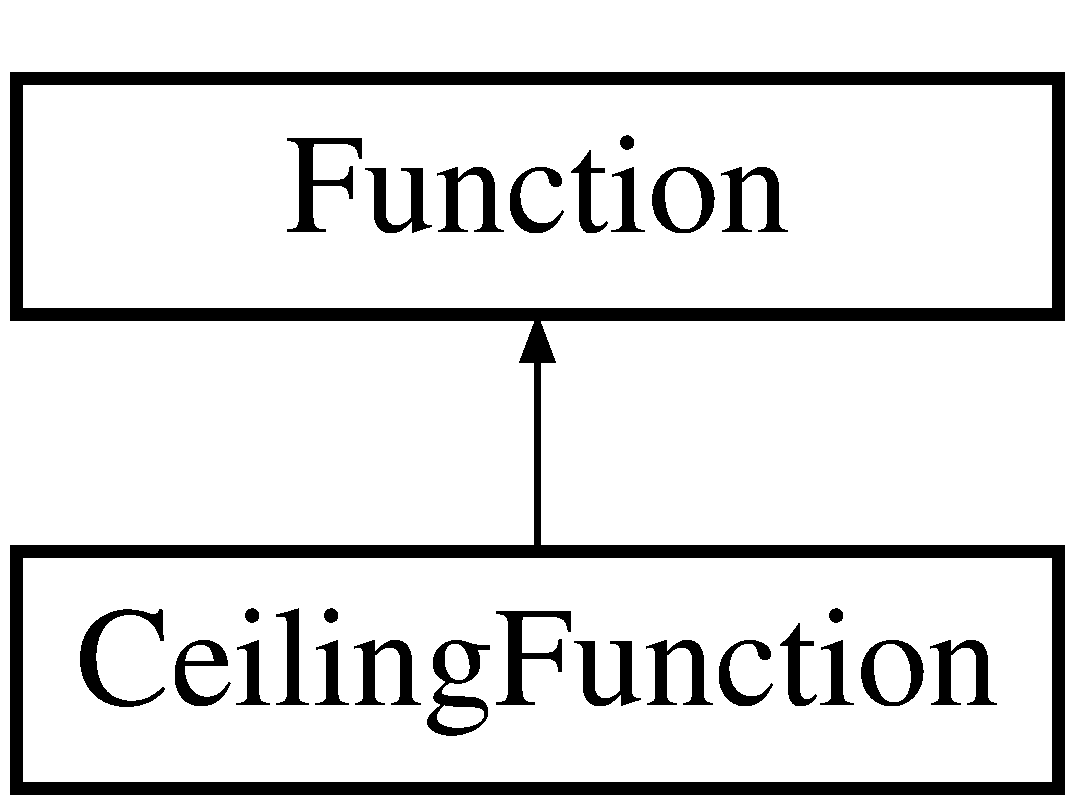
\includegraphics[height=2.000000cm]{class_ceiling_function}
\end{center}
\end{figure}
\subsection*{Public Member Functions}
\begin{DoxyCompactItemize}
\item 
virtual Decimal \hyperlink{class_ceiling_function_a5aac31296f54c9af13acfbe2dc8559d2}{value\+At} (Decimal x) const 
\begin{DoxyCompactList}\small\item\em Method to determine the value of \hyperlink{class_ceiling_function}{Ceiling\+Function}. \end{DoxyCompactList}\end{DoxyCompactItemize}


\subsection{Detailed Description}
\hyperlink{class_function}{Function} to compute the mathematical ceiling of the input. 

\subsection{Member Function Documentation}
\hypertarget{class_ceiling_function_a5aac31296f54c9af13acfbe2dc8559d2}{\index{Ceiling\+Function@{Ceiling\+Function}!value\+At@{value\+At}}
\index{value\+At@{value\+At}!Ceiling\+Function@{Ceiling\+Function}}
\subsubsection[{value\+At}]{\setlength{\rightskip}{0pt plus 5cm}virtual Decimal Ceiling\+Function\+::value\+At (
\begin{DoxyParamCaption}
\item[{Decimal}]{x}
\end{DoxyParamCaption}
) const\hspace{0.3cm}{\ttfamily [inline]}, {\ttfamily [virtual]}}}\label{class_ceiling_function_a5aac31296f54c9af13acfbe2dc8559d2}


Method to determine the value of \hyperlink{class_ceiling_function}{Ceiling\+Function}. 

\begin{DoxyReturn}{Returns}
The smallest integer greater than or equal to {\itshape x}. 
\end{DoxyReturn}


Implements \hyperlink{class_function_a7773feae8f1def0a2d7e479363700816}{Function}.



The documentation for this class was generated from the following file\+:\begin{DoxyCompactItemize}
\item 
Function.\+h\end{DoxyCompactItemize}

\hypertarget{class_colored_polygon}{\section{Colored\+Polygon Class Reference}
\label{class_colored_polygon}\index{Colored\+Polygon@{Colored\+Polygon}}
}


Draw an arbitrary polygon with colored vertices.  




{\ttfamily \#include $<$Colored\+Polygon.\+h$>$}

Inheritance diagram for Colored\+Polygon\+:\begin{figure}[H]
\begin{center}
\leavevmode
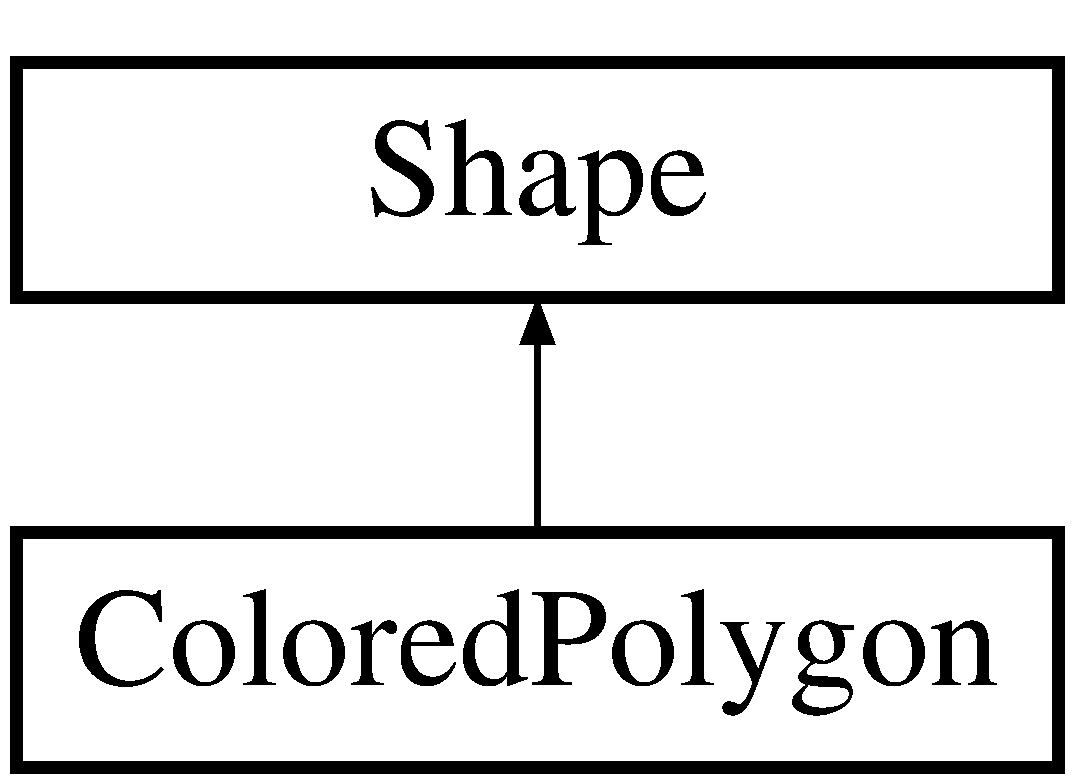
\includegraphics[height=2.000000cm]{class_colored_polygon}
\end{center}
\end{figure}
\subsection*{Public Member Functions}
\begin{DoxyCompactItemize}
\item 
\hyperlink{class_colored_polygon_aa532110241b18425555fed1dc18937c0}{Colored\+Polygon} (int v)
\begin{DoxyCompactList}\small\item\em Explicitly constructor a new \hyperlink{class_colored_polygon}{Colored\+Polygon}. \end{DoxyCompactList}\item 
void \hyperlink{class_colored_polygon_ab0791f2c340d92ac452fdd96aa0fcde0}{add\+Vertex} (int x, int y, const \hyperlink{struct_color_float}{Color\+Float} \&color)
\begin{DoxyCompactList}\small\item\em Add another vertex to the \hyperlink{class_colored_polygon}{Colored\+Polygon}. \end{DoxyCompactList}\item 
void \hyperlink{class_colored_polygon_a543a3233225455e9288b0b98735fab42}{draw} ()
\begin{DoxyCompactList}\small\item\em Draw the \hyperlink{class_colored_polygon}{Colored\+Polygon}. \end{DoxyCompactList}\end{DoxyCompactItemize}
\subsection*{Additional Inherited Members}


\subsection{Detailed Description}
Draw an arbitrary polygon with colored vertices. 

\hyperlink{class_colored_polygon}{Colored\+Polygon} is a class for holding vertex data for a triangle strip with colored vertices.

Vertices are drawn in triangle strip format, where the first three vertices make up the first triangle, the next vertex plus the previous two make up the second triangle, and so on.

This method is optimized for long lists and offers a marked improvement over drawing individual \hyperlink{class_triangle}{Triangle} instances. \begin{DoxyNote}{Note}
The \hyperlink{class_colored_polygon_ab0791f2c340d92ac452fdd96aa0fcde0}{add\+Vertex()} method must be called the same number of times as specified in the constructor. 

Calling \hyperlink{class_colored_polygon_ab0791f2c340d92ac452fdd96aa0fcde0}{add\+Vertex()} after all vertices have been added will do nothing. 

Calling \hyperlink{class_colored_polygon_a543a3233225455e9288b0b98735fab42}{draw()} before all vertices have been added will do nothing. 
\end{DoxyNote}


\subsection{Constructor \& Destructor Documentation}
\hypertarget{class_colored_polygon_aa532110241b18425555fed1dc18937c0}{\index{Colored\+Polygon@{Colored\+Polygon}!Colored\+Polygon@{Colored\+Polygon}}
\index{Colored\+Polygon@{Colored\+Polygon}!Colored\+Polygon@{Colored\+Polygon}}
\subsubsection[{Colored\+Polygon}]{\setlength{\rightskip}{0pt plus 5cm}Colored\+Polygon\+::\+Colored\+Polygon (
\begin{DoxyParamCaption}
\item[{int}]{v}
\end{DoxyParamCaption}
)}}\label{class_colored_polygon_aa532110241b18425555fed1dc18937c0}


Explicitly constructor a new \hyperlink{class_colored_polygon}{Colored\+Polygon}. 


\begin{DoxyParams}{Parameters}
{\em v,the} & number of vertices the complete \hyperlink{class_colored_polygon}{Colored\+Polygon} will have. \\
\hline
\end{DoxyParams}
\begin{DoxyReturn}{Returns}
a new \hyperlink{class_colored_polygon}{Colored\+Polygon} with a buffer for storing the specified numbered of vertices. 
\end{DoxyReturn}


\subsection{Member Function Documentation}
\hypertarget{class_colored_polygon_ab0791f2c340d92ac452fdd96aa0fcde0}{\index{Colored\+Polygon@{Colored\+Polygon}!add\+Vertex@{add\+Vertex}}
\index{add\+Vertex@{add\+Vertex}!Colored\+Polygon@{Colored\+Polygon}}
\subsubsection[{add\+Vertex}]{\setlength{\rightskip}{0pt plus 5cm}void Colored\+Polygon\+::add\+Vertex (
\begin{DoxyParamCaption}
\item[{int}]{x, }
\item[{int}]{y, }
\item[{const {\bf Color\+Float} \&}]{color}
\end{DoxyParamCaption}
)}}\label{class_colored_polygon_ab0791f2c340d92ac452fdd96aa0fcde0}


Add another vertex to the \hyperlink{class_colored_polygon}{Colored\+Polygon}. 

This function initalizes the next vertex in the \hyperlink{class_polyline}{Polyline} and adds it to the \hyperlink{class_colored_polygon}{Colored\+Polygon} buffer. 
\begin{DoxyParams}{Parameters}
{\em x} & The x position of the vertex. \\
\hline
{\em y} & The y position of the vertex. \\
\hline
{\em color} & The color of the vertex. \\
\hline
\end{DoxyParams}
\begin{DoxyNote}{Note}
This function does nothing if the vertex buffer is already full. 
\end{DoxyNote}


Referenced by Canvas\+::draw\+Circle(), and Canvas\+::draw\+Colored\+Polygon().

\hypertarget{class_colored_polygon_a543a3233225455e9288b0b98735fab42}{\index{Colored\+Polygon@{Colored\+Polygon}!draw@{draw}}
\index{draw@{draw}!Colored\+Polygon@{Colored\+Polygon}}
\subsubsection[{draw}]{\setlength{\rightskip}{0pt plus 5cm}void Colored\+Polygon\+::draw (
\begin{DoxyParamCaption}
{}
\end{DoxyParamCaption}
)\hspace{0.3cm}{\ttfamily [virtual]}}}\label{class_colored_polygon_a543a3233225455e9288b0b98735fab42}


Draw the \hyperlink{class_colored_polygon}{Colored\+Polygon}. 

This function actually draws the \hyperlink{class_colored_polygon}{Colored\+Polygon} to the \hyperlink{class_canvas}{Canvas}. \begin{DoxyNote}{Note}
This function does nothing if the vertex buffer is not yet full. 
\end{DoxyNote}


Implements \hyperlink{class_shape_afacc5aad8e37308c3ce8fef768199b05}{Shape}.



The documentation for this class was generated from the following files\+:\begin{DoxyCompactItemize}
\item 
Colored\+Polygon.\+h\item 
Colored\+Polygon.\+cpp\end{DoxyCompactItemize}

\hypertarget{struct_color_float}{\section{Color\+Float Struct Reference}
\label{struct_color_float}\index{Color\+Float@{Color\+Float}}
}


Floating point R\+G\+B\+A color struct.  




{\ttfamily \#include $<$Color.\+h$>$}

\subsection*{Public Member Functions}
\begin{DoxyCompactItemize}
\item 
\hypertarget{struct_color_float_a035529117ce865b9208aa429f9a97444}{{\bfseries Color\+Float} (float r, float g, float b, float a=1.\+0f)}\label{struct_color_float_a035529117ce865b9208aa429f9a97444}

\end{DoxyCompactItemize}
\subsection*{Public Attributes}
\begin{DoxyCompactItemize}
\item 
\hypertarget{struct_color_float_a03a281944228fa7de5251633c0c270c7}{float {\bfseries R}}\label{struct_color_float_a03a281944228fa7de5251633c0c270c7}

\item 
\hypertarget{struct_color_float_a6c8d0d5307f56ab8d298cfb4246b5c08}{float {\bfseries G}}\label{struct_color_float_a6c8d0d5307f56ab8d298cfb4246b5c08}

\item 
\hypertarget{struct_color_float_a12bb7d32004e66d2063093bccd87dd72}{float {\bfseries B}}\label{struct_color_float_a12bb7d32004e66d2063093bccd87dd72}

\item 
\hypertarget{struct_color_float_a518c16e83cea9c578964377499015b20}{float {\bfseries A}}\label{struct_color_float_a518c16e83cea9c578964377499015b20}

\end{DoxyCompactItemize}


\subsection{Detailed Description}
Floating point R\+G\+B\+A color struct. 

\hyperlink{struct_color_float}{Color\+Float} defines a color with floating point red, green, blue, and alpha components 
\begin{DoxyParams}{Parameters}
{\em R} & Red component, between 0 and 1 inclusive. \\
\hline
{\em G} & Green component, between 0 and 1 inclusive. \\
\hline
{\em B} & Blue component, between 0 and 1 inclusive. \\
\hline
{\em A} & Alpha component, between 0 and 1 inclusive. \\
\hline
\end{DoxyParams}


The documentation for this struct was generated from the following files\+:\begin{DoxyCompactItemize}
\item 
Color.\+h\item 
Color.\+cpp\end{DoxyCompactItemize}

\hypertarget{struct_color_h_s_v}{\section{Color\+H\+S\+V Struct Reference}
\label{struct_color_h_s_v}\index{Color\+H\+S\+V@{Color\+H\+S\+V}}
}


Floating pont H\+S\+V\+A color struct.  




{\ttfamily \#include $<$Color.\+h$>$}

\subsection*{Public Member Functions}
\begin{DoxyCompactItemize}
\item 
\hypertarget{struct_color_h_s_v_ab5add9e01e8d363874bcba5c7908e4bf}{{\bfseries Color\+H\+S\+V} (float h, float s, float v, float a=1.\+0f)}\label{struct_color_h_s_v_ab5add9e01e8d363874bcba5c7908e4bf}

\item 
\hyperlink{struct_color_h_s_v_a7a528f702f78a761a852459865d0f315}{operator Color\+Float} ()
\begin{DoxyCompactList}\small\item\em Implicit conversion from \hyperlink{struct_color_h_s_v}{Color\+H\+S\+V} to \hyperlink{struct_color_float}{Color\+Float}. \end{DoxyCompactList}\end{DoxyCompactItemize}
\subsection*{Public Attributes}
\begin{DoxyCompactItemize}
\item 
\hypertarget{struct_color_h_s_v_aa89f54beecbbbfc1aa2fc052841df10a}{float {\bfseries H}}\label{struct_color_h_s_v_aa89f54beecbbbfc1aa2fc052841df10a}

\item 
\hypertarget{struct_color_h_s_v_a3b1b00fc23b90d9dd708ae34225b9b27}{float {\bfseries S}}\label{struct_color_h_s_v_a3b1b00fc23b90d9dd708ae34225b9b27}

\item 
\hypertarget{struct_color_h_s_v_aeb5ccdbb997f9988b57dc17e92c5e08a}{float {\bfseries V}}\label{struct_color_h_s_v_aeb5ccdbb997f9988b57dc17e92c5e08a}

\item 
\hypertarget{struct_color_h_s_v_a64e94b0c42d2d328fd720dd3b0e60860}{float {\bfseries A}}\label{struct_color_h_s_v_a64e94b0c42d2d328fd720dd3b0e60860}

\end{DoxyCompactItemize}


\subsection{Detailed Description}
Floating pont H\+S\+V\+A color struct. 

\hyperlink{struct_color_h_s_v}{Color\+H\+S\+V} defines a color with floating point hue, saturation, value, and alpha components 
\begin{DoxyParams}{Parameters}
{\em H} & Hue component, between 0 and 6 inclusive. \\
\hline
{\em S} & Saturation component, between 0 and 1 inclusive. \\
\hline
{\em V} & Value component, between 0 and 1 inclusive. \\
\hline
{\em A} & Alpha component, between 0 and 1 inclusive. \\
\hline
\end{DoxyParams}


\subsection{Member Function Documentation}
\hypertarget{struct_color_h_s_v_a7a528f702f78a761a852459865d0f315}{\index{Color\+H\+S\+V@{Color\+H\+S\+V}!operator Color\+Float@{operator Color\+Float}}
\index{operator Color\+Float@{operator Color\+Float}!Color\+H\+S\+V@{Color\+H\+S\+V}}
\subsubsection[{operator Color\+Float}]{\setlength{\rightskip}{0pt plus 5cm}Color\+H\+S\+V\+::operator {\bf Color\+Float} (
\begin{DoxyParamCaption}
{}
\end{DoxyParamCaption}
)}}\label{struct_color_h_s_v_a7a528f702f78a761a852459865d0f315}


Implicit conversion from \hyperlink{struct_color_h_s_v}{Color\+H\+S\+V} to \hyperlink{struct_color_float}{Color\+Float}. 

This defines the implicit conversion operator from an H\+S\+V color type (\hyperlink{struct_color_h_s_v}{Color\+H\+S\+V}) to an R\+G\+B color type (\hyperlink{struct_color_float}{Color\+Float}) 

The documentation for this struct was generated from the following files\+:\begin{DoxyCompactItemize}
\item 
Color.\+h\item 
Color.\+cpp\end{DoxyCompactItemize}

\hypertarget{struct_color_int}{\section{Color\+Int Struct Reference}
\label{struct_color_int}\index{Color\+Int@{Color\+Int}}
}


Integer R\+G\+B\+A color struct.  




{\ttfamily \#include $<$Color.\+h$>$}

\subsection*{Public Member Functions}
\begin{DoxyCompactItemize}
\item 
\hypertarget{struct_color_int_ad9eef03a92353332dc3c46cb1ba5071d}{{\bfseries Color\+Int} (int r, int g, int b, int a=255)}\label{struct_color_int_ad9eef03a92353332dc3c46cb1ba5071d}

\item 
\hyperlink{struct_color_int_a7a0bec01fc87ef256cd15bd2e51f55ff}{operator Color\+Float} ()
\begin{DoxyCompactList}\small\item\em Implicit conversion from \hyperlink{struct_color_int}{Color\+Int} to \hyperlink{struct_color_float}{Color\+Float}. \end{DoxyCompactList}\end{DoxyCompactItemize}
\subsection*{Public Attributes}
\begin{DoxyCompactItemize}
\item 
\hypertarget{struct_color_int_a49487fa834ef54da91085bb0346109da}{int {\bfseries R}}\label{struct_color_int_a49487fa834ef54da91085bb0346109da}

\item 
\hypertarget{struct_color_int_aa0b690191e8267e2699561b8526e04c9}{int {\bfseries G}}\label{struct_color_int_aa0b690191e8267e2699561b8526e04c9}

\item 
\hypertarget{struct_color_int_a49ef255f3a8e47b3a1b990eace30e894}{int {\bfseries B}}\label{struct_color_int_a49ef255f3a8e47b3a1b990eace30e894}

\item 
\hypertarget{struct_color_int_a5f3064ef16e526140807800b86affd18}{int {\bfseries A}}\label{struct_color_int_a5f3064ef16e526140807800b86affd18}

\end{DoxyCompactItemize}


\subsection{Detailed Description}
Integer R\+G\+B\+A color struct. 

\hyperlink{struct_color_int}{Color\+Int} defines a color with integer red, green, blue, and alpha components 
\begin{DoxyParams}{Parameters}
{\em R} & Red component, between 0 and 255 inclusive. \\
\hline
{\em G} & Green component, between 0 and 255 inclusive. \\
\hline
{\em B} & Blue component, between 0 and 255 inclusive. \\
\hline
{\em A} & Alpha component, between 0 and 255 inclusive. \\
\hline
\end{DoxyParams}


\subsection{Member Function Documentation}
\hypertarget{struct_color_int_a7a0bec01fc87ef256cd15bd2e51f55ff}{\index{Color\+Int@{Color\+Int}!operator Color\+Float@{operator Color\+Float}}
\index{operator Color\+Float@{operator Color\+Float}!Color\+Int@{Color\+Int}}
\subsubsection[{operator Color\+Float}]{\setlength{\rightskip}{0pt plus 5cm}Color\+Int\+::operator {\bf Color\+Float} (
\begin{DoxyParamCaption}
{}
\end{DoxyParamCaption}
)}}\label{struct_color_int_a7a0bec01fc87ef256cd15bd2e51f55ff}


Implicit conversion from \hyperlink{struct_color_int}{Color\+Int} to \hyperlink{struct_color_float}{Color\+Float}. 

This defines the implicit conversion operator from an integer color type (\hyperlink{struct_color_int}{Color\+Int}) to a floating point color type (\hyperlink{struct_color_float}{Color\+Float}) 

The documentation for this struct was generated from the following files\+:\begin{DoxyCompactItemize}
\item 
Color.\+h\item 
Color.\+cpp\end{DoxyCompactItemize}

\hypertarget{class_colors}{\section{Colors Class Reference}
\label{class_colors}\index{Colors@{Colors}}
}


Color utility class.  




{\ttfamily \#include $<$Color.\+h$>$}

\subsection*{Static Public Member Functions}
\begin{DoxyCompactItemize}
\item 
static \hyperlink{struct_color_float}{Color\+Float} \hyperlink{class_colors_a9d471a8fb06c0aac407de2945c1c65c6}{divide\+Into\+Chromatic\+Sections} (unsigned int sections, unsigned int section, float value, float alpha=1.\+0f)
\begin{DoxyCompactList}\small\item\em Returns an H\+S\+V\+A color with a hue dependent on the number of sections. \end{DoxyCompactList}\item 
static \hyperlink{struct_color_float}{Color\+Float} \hyperlink{class_colors_ad8312b55a80fb26bb20a80e8af8d3f1a}{divide\+Into\+Chromatic\+Sections} (unsigned int sections, unsigned int section)
\begin{DoxyCompactList}\small\item\em Returns an H\+S\+V\+A color with a hue dependent on the number of sections. \end{DoxyCompactList}\item 
static \hyperlink{struct_color_float}{Color\+Float} \hyperlink{class_colors_a3155080f6bbee603212059a8f4abe6f3}{random\+Color} (float alpha=0.\+0f)
\begin{DoxyCompactList}\small\item\em Generates a random color. \end{DoxyCompactList}\item 
static \hyperlink{struct_color_float}{Color\+Float} \hyperlink{class_colors_ae24518e4d2618cc5a670316f6d53f844}{blended\+Color} (\hyperlink{struct_color_float}{Color\+Float} c1, \hyperlink{struct_color_float}{Color\+Float} c2, float bias)
\begin{DoxyCompactList}\small\item\em Blends two colors with a given bias towards the latter. \end{DoxyCompactList}\item 
\hypertarget{class_colors_ae43bb23e649eb2a5a9fd9e34f25092f7}{static \hyperlink{struct_color_float}{Color\+Float} {\bfseries high\+Contrast\+Color} (unsigned int section, int seed=0)}\label{class_colors_ae43bb23e649eb2a5a9fd9e34f25092f7}

\end{DoxyCompactItemize}


\subsection{Detailed Description}
Color utility class. 

\hyperlink{class_colors}{Colors} defines color utility methods to construct colors. 

\subsection{Member Function Documentation}
\hypertarget{class_colors_ae24518e4d2618cc5a670316f6d53f844}{\index{Colors@{Colors}!blended\+Color@{blended\+Color}}
\index{blended\+Color@{blended\+Color}!Colors@{Colors}}
\subsubsection[{blended\+Color}]{\setlength{\rightskip}{0pt plus 5cm}{\bf Color\+Float} Colors\+::blended\+Color (
\begin{DoxyParamCaption}
\item[{{\bf Color\+Float}}]{c1, }
\item[{{\bf Color\+Float}}]{c2, }
\item[{float}]{bias}
\end{DoxyParamCaption}
)\hspace{0.3cm}{\ttfamily [static]}}}\label{class_colors_ae24518e4d2618cc5a670316f6d53f844}


Blends two colors with a given bias towards the latter. 

This function blends two \hyperlink{struct_color_float}{Color\+Float} structs together by taking a linear interpolation between the two and returns the result as a new \hyperlink{struct_color_float}{Color\+Float}. 
\begin{DoxyParams}{Parameters}
{\em c1} & A \hyperlink{struct_color_float}{Color\+Float}. \\
\hline
{\em c2} & Another \hyperlink{struct_color_float}{Color\+Float}. \\
\hline
{\em bias} & A bias between 0 and 1 inclusive. A bias of 0 returns c1, a bias of 1 returns c2, and a bias in between returns a linear interpolation. \\
\hline
\end{DoxyParams}
\begin{DoxyReturn}{Returns}
A \hyperlink{struct_color_float}{Color\+Float} linearly interpolated between c1 and c2 using the given bias as a weight. 
\end{DoxyReturn}
\hypertarget{class_colors_a9d471a8fb06c0aac407de2945c1c65c6}{\index{Colors@{Colors}!divide\+Into\+Chromatic\+Sections@{divide\+Into\+Chromatic\+Sections}}
\index{divide\+Into\+Chromatic\+Sections@{divide\+Into\+Chromatic\+Sections}!Colors@{Colors}}
\subsubsection[{divide\+Into\+Chromatic\+Sections}]{\setlength{\rightskip}{0pt plus 5cm}{\bf Color\+Float} Colors\+::divide\+Into\+Chromatic\+Sections (
\begin{DoxyParamCaption}
\item[{unsigned int}]{sections, }
\item[{unsigned int}]{section, }
\item[{float}]{value, }
\item[{float}]{alpha = {\ttfamily 1.0f}}
\end{DoxyParamCaption}
)\hspace{0.3cm}{\ttfamily [static]}}}\label{class_colors_a9d471a8fb06c0aac407de2945c1c65c6}


Returns an H\+S\+V\+A color with a hue dependent on the number of sections. 

This function returns a \hyperlink{struct_color_float}{Color\+Float} whose hue is calculated from the provided section number and the total number of sections. This function is used for creating a chromatic gradient from one part of the spectrum to another. 
\begin{DoxyParams}{Parameters}
{\em section} & Integer specifying the current section. \\
\hline
{\em sections} & Integer specifying the total number of sections. \\
\hline
{\em value} & Value component, between 0 and 1 inclusive. \\
\hline
{\em alpha} & Alpha component, between 0 and 1 inclusive. \\
\hline
\end{DoxyParams}
\begin{DoxyReturn}{Returns}
A \hyperlink{struct_color_float}{Color\+Float} with a hue calculated as 6.\+0f/sections$\ast$section, saturation of 1.\+0, and the given value and alpha components. 
\end{DoxyReturn}


Referenced by divide\+Into\+Chromatic\+Sections().

\hypertarget{class_colors_ad8312b55a80fb26bb20a80e8af8d3f1a}{\index{Colors@{Colors}!divide\+Into\+Chromatic\+Sections@{divide\+Into\+Chromatic\+Sections}}
\index{divide\+Into\+Chromatic\+Sections@{divide\+Into\+Chromatic\+Sections}!Colors@{Colors}}
\subsubsection[{divide\+Into\+Chromatic\+Sections}]{\setlength{\rightskip}{0pt plus 5cm}{\bf Color\+Float} Colors\+::divide\+Into\+Chromatic\+Sections (
\begin{DoxyParamCaption}
\item[{unsigned int}]{sections, }
\item[{unsigned int}]{section}
\end{DoxyParamCaption}
)\hspace{0.3cm}{\ttfamily [static]}}}\label{class_colors_ad8312b55a80fb26bb20a80e8af8d3f1a}


Returns an H\+S\+V\+A color with a hue dependent on the number of sections. 

This function returns a \hyperlink{struct_color_float}{Color\+Float} whose hue is calculated from the provided section number and the total number of sections. This function is used for creating a chromatic gradient from one part of the spectrum to another. 
\begin{DoxyParams}{Parameters}
{\em section} & Integer specifying the current section. \\
\hline
{\em sections} & Integer specifying the total number of sections. \\
\hline
\end{DoxyParams}
\begin{DoxyReturn}{Returns}
A \hyperlink{struct_color_float}{Color\+Float} with a hue calculated as 6.\+0f/sections$\ast$section, and a saturation, value, and alpha of 1.\+0. 
\end{DoxyReturn}
\hypertarget{class_colors_a3155080f6bbee603212059a8f4abe6f3}{\index{Colors@{Colors}!random\+Color@{random\+Color}}
\index{random\+Color@{random\+Color}!Colors@{Colors}}
\subsubsection[{random\+Color}]{\setlength{\rightskip}{0pt plus 5cm}{\bf Color\+Float} Colors\+::random\+Color (
\begin{DoxyParamCaption}
\item[{float}]{alpha = {\ttfamily 0.0f}}
\end{DoxyParamCaption}
)\hspace{0.3cm}{\ttfamily [static]}}}\label{class_colors_a3155080f6bbee603212059a8f4abe6f3}


Generates a random color. 

This function user rand() to generate a random \hyperlink{struct_color_float}{Color\+Float} with an optional specified alpha value. 
\begin{DoxyParams}{Parameters}
{\em alpha} & Alpha of the random color to generate. An alpha of 0 will set the alpha to a random legal value. \\
\hline
\end{DoxyParams}
\begin{DoxyReturn}{Returns}
A random \hyperlink{struct_color_float}{Color\+Float}. 
\end{DoxyReturn}


The documentation for this class was generated from the following files\+:\begin{DoxyCompactItemize}
\item 
Color.\+h\item 
Color.\+cpp\end{DoxyCompactItemize}

\hypertarget{class_common_log_function}{\section{Common\+Log\+Function Class Reference}
\label{class_common_log_function}\index{Common\+Log\+Function@{Common\+Log\+Function}}
}


\hyperlink{class_function}{Function} to compute the base 10 log of the input.  




{\ttfamily \#include $<$Function.\+h$>$}

Inheritance diagram for Common\+Log\+Function\+:\begin{figure}[H]
\begin{center}
\leavevmode
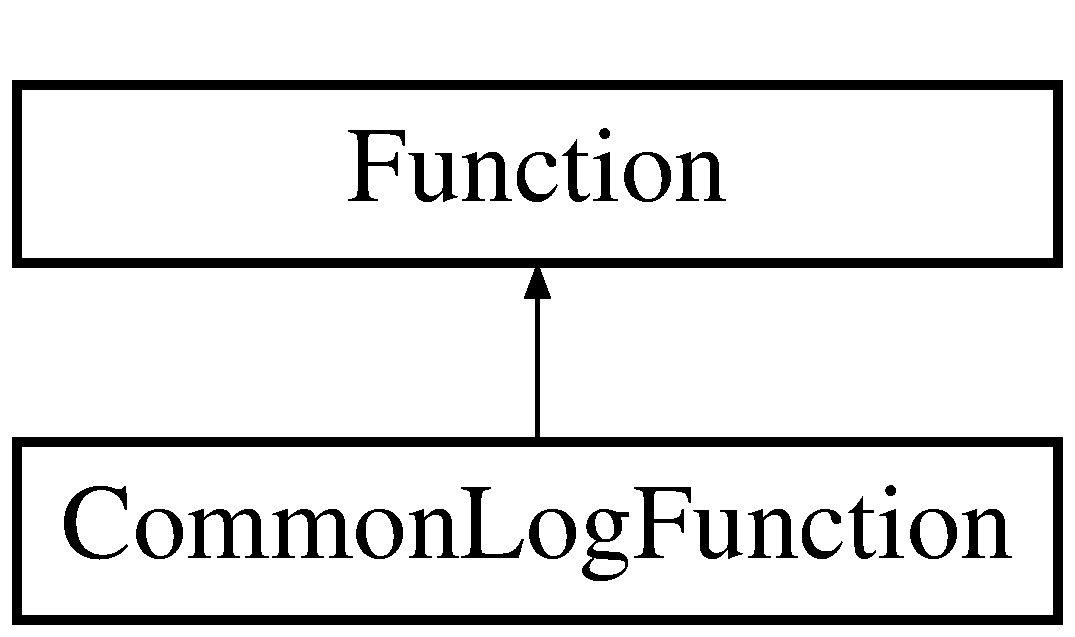
\includegraphics[height=2.000000cm]{class_common_log_function}
\end{center}
\end{figure}
\subsection*{Public Member Functions}
\begin{DoxyCompactItemize}
\item 
virtual Decimal \hyperlink{class_common_log_function_a96f716f78cdab4c5458f8372424b52a4}{value\+At} (Decimal x) const 
\begin{DoxyCompactList}\small\item\em Method to determine the value of \hyperlink{class_common_log_function}{Common\+Log\+Function}. \end{DoxyCompactList}\end{DoxyCompactItemize}


\subsection{Detailed Description}
\hyperlink{class_function}{Function} to compute the base 10 log of the input. 

\subsection{Member Function Documentation}
\hypertarget{class_common_log_function_a96f716f78cdab4c5458f8372424b52a4}{\index{Common\+Log\+Function@{Common\+Log\+Function}!value\+At@{value\+At}}
\index{value\+At@{value\+At}!Common\+Log\+Function@{Common\+Log\+Function}}
\subsubsection[{value\+At}]{\setlength{\rightskip}{0pt plus 5cm}virtual Decimal Common\+Log\+Function\+::value\+At (
\begin{DoxyParamCaption}
\item[{Decimal}]{x}
\end{DoxyParamCaption}
) const\hspace{0.3cm}{\ttfamily [inline]}, {\ttfamily [virtual]}}}\label{class_common_log_function_a96f716f78cdab4c5458f8372424b52a4}


Method to determine the value of \hyperlink{class_common_log_function}{Common\+Log\+Function}. 

\begin{DoxyReturn}{Returns}
The base 10 log of {\itshape x}. 
\end{DoxyReturn}


Implements \hyperlink{class_function_a7773feae8f1def0a2d7e479363700816}{Function}.



The documentation for this class was generated from the following file\+:\begin{DoxyCompactItemize}
\item 
Function.\+h\end{DoxyCompactItemize}

\hypertarget{class_cosine_function}{\section{Cosine\+Function Class Reference}
\label{class_cosine_function}\index{Cosine\+Function@{Cosine\+Function}}
}


\hyperlink{class_function}{Function} to compute the cosine of the input.  




{\ttfamily \#include $<$Function.\+h$>$}

Inheritance diagram for Cosine\+Function\+:\begin{figure}[H]
\begin{center}
\leavevmode
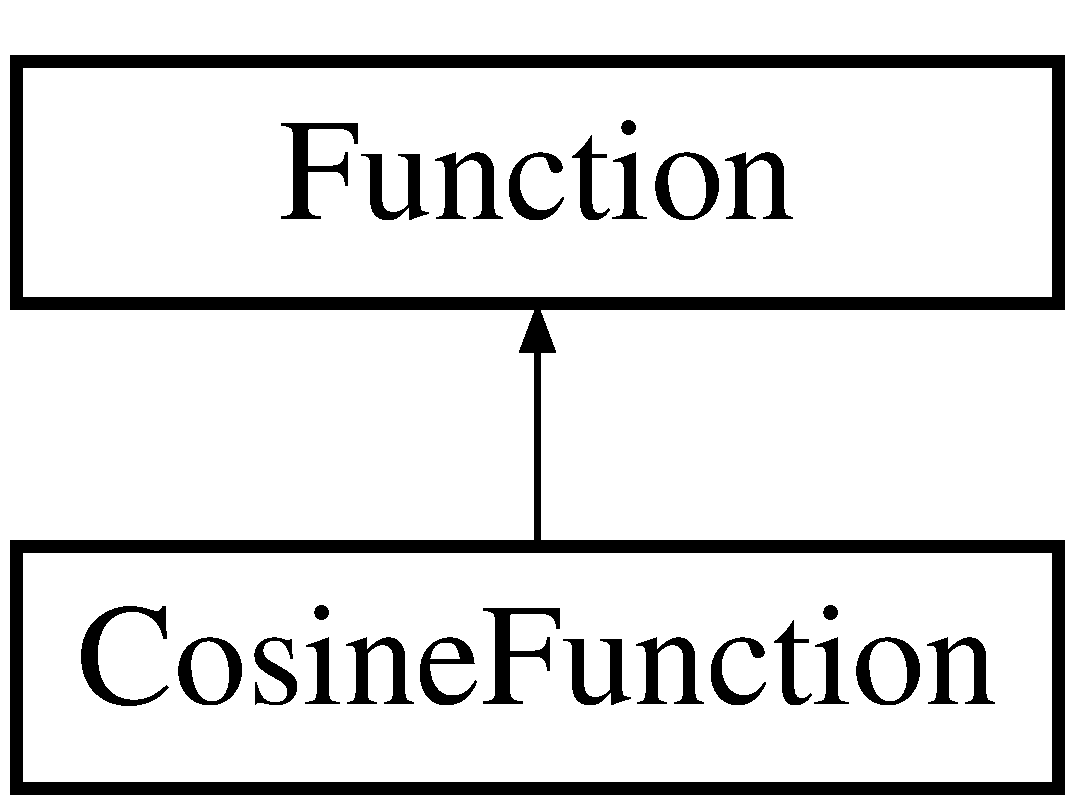
\includegraphics[height=2.000000cm]{class_cosine_function}
\end{center}
\end{figure}
\subsection*{Public Member Functions}
\begin{DoxyCompactItemize}
\item 
virtual Decimal \hyperlink{class_cosine_function_a0a0a5067e129d5183b17d4f0bfffd435}{value\+At} (Decimal x) const 
\begin{DoxyCompactList}\small\item\em Method to determine the value of \hyperlink{class_cosine_function}{Cosine\+Function}. \end{DoxyCompactList}\end{DoxyCompactItemize}


\subsection{Detailed Description}
\hyperlink{class_function}{Function} to compute the cosine of the input. 

\subsection{Member Function Documentation}
\hypertarget{class_cosine_function_a0a0a5067e129d5183b17d4f0bfffd435}{\index{Cosine\+Function@{Cosine\+Function}!value\+At@{value\+At}}
\index{value\+At@{value\+At}!Cosine\+Function@{Cosine\+Function}}
\subsubsection[{value\+At}]{\setlength{\rightskip}{0pt plus 5cm}virtual Decimal Cosine\+Function\+::value\+At (
\begin{DoxyParamCaption}
\item[{Decimal}]{x}
\end{DoxyParamCaption}
) const\hspace{0.3cm}{\ttfamily [inline]}, {\ttfamily [virtual]}}}\label{class_cosine_function_a0a0a5067e129d5183b17d4f0bfffd435}


Method to determine the value of \hyperlink{class_cosine_function}{Cosine\+Function}. 

\begin{DoxyReturn}{Returns}
The cosine of {\itshape x}. 
\end{DoxyReturn}


Implements \hyperlink{class_function_a7773feae8f1def0a2d7e479363700816}{Function}.



The documentation for this class was generated from the following file\+:\begin{DoxyCompactItemize}
\item 
Function.\+h\end{DoxyCompactItemize}

\hypertarget{class_exponential_function}{\section{Exponential\+Function Class Reference}
\label{class_exponential_function}\index{Exponential\+Function@{Exponential\+Function}}
}


\hyperlink{class_function}{Function} to compute e raised to the input.  




{\ttfamily \#include $<$Function.\+h$>$}

Inheritance diagram for Exponential\+Function\+:\begin{figure}[H]
\begin{center}
\leavevmode
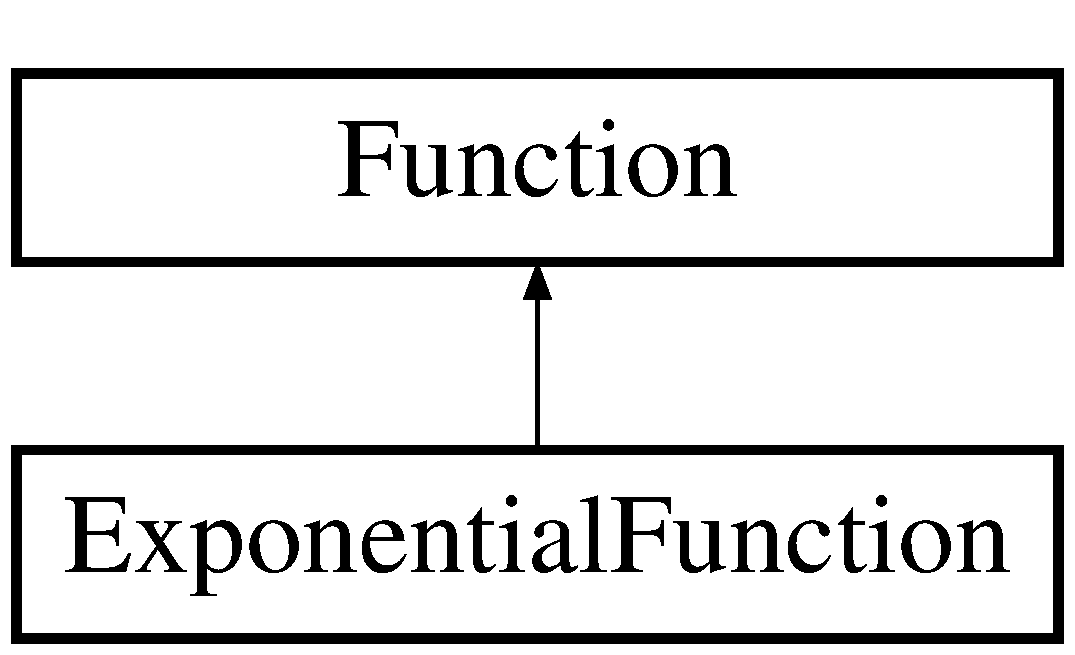
\includegraphics[height=2.000000cm]{class_exponential_function}
\end{center}
\end{figure}
\subsection*{Public Member Functions}
\begin{DoxyCompactItemize}
\item 
virtual Decimal \hyperlink{class_exponential_function_acb8ed2181be3fa4082a8ff3a61e711a1}{value\+At} (Decimal x) const 
\begin{DoxyCompactList}\small\item\em Method to determine the value of \hyperlink{class_exponential_function}{Exponential\+Function}. \end{DoxyCompactList}\end{DoxyCompactItemize}


\subsection{Detailed Description}
\hyperlink{class_function}{Function} to compute e raised to the input. 

\subsection{Member Function Documentation}
\hypertarget{class_exponential_function_acb8ed2181be3fa4082a8ff3a61e711a1}{\index{Exponential\+Function@{Exponential\+Function}!value\+At@{value\+At}}
\index{value\+At@{value\+At}!Exponential\+Function@{Exponential\+Function}}
\subsubsection[{value\+At}]{\setlength{\rightskip}{0pt plus 5cm}virtual Decimal Exponential\+Function\+::value\+At (
\begin{DoxyParamCaption}
\item[{Decimal}]{x}
\end{DoxyParamCaption}
) const\hspace{0.3cm}{\ttfamily [inline]}, {\ttfamily [virtual]}}}\label{class_exponential_function_acb8ed2181be3fa4082a8ff3a61e711a1}


Method to determine the value of \hyperlink{class_exponential_function}{Exponential\+Function}. 

\begin{DoxyReturn}{Returns}
{\itshape e} raised to the power of {\itshape x}. 
\end{DoxyReturn}


Implements \hyperlink{class_function_a7773feae8f1def0a2d7e479363700816}{Function}.



The documentation for this class was generated from the following file\+:\begin{DoxyCompactItemize}
\item 
Function.\+h\end{DoxyCompactItemize}

\hypertarget{class_floor_function}{\section{Floor\+Function Class Reference}
\label{class_floor_function}\index{Floor\+Function@{Floor\+Function}}
}


\hyperlink{class_function}{Function} to compute the mathematical floor of the input.  




{\ttfamily \#include $<$Function.\+h$>$}

Inheritance diagram for Floor\+Function\+:\begin{figure}[H]
\begin{center}
\leavevmode
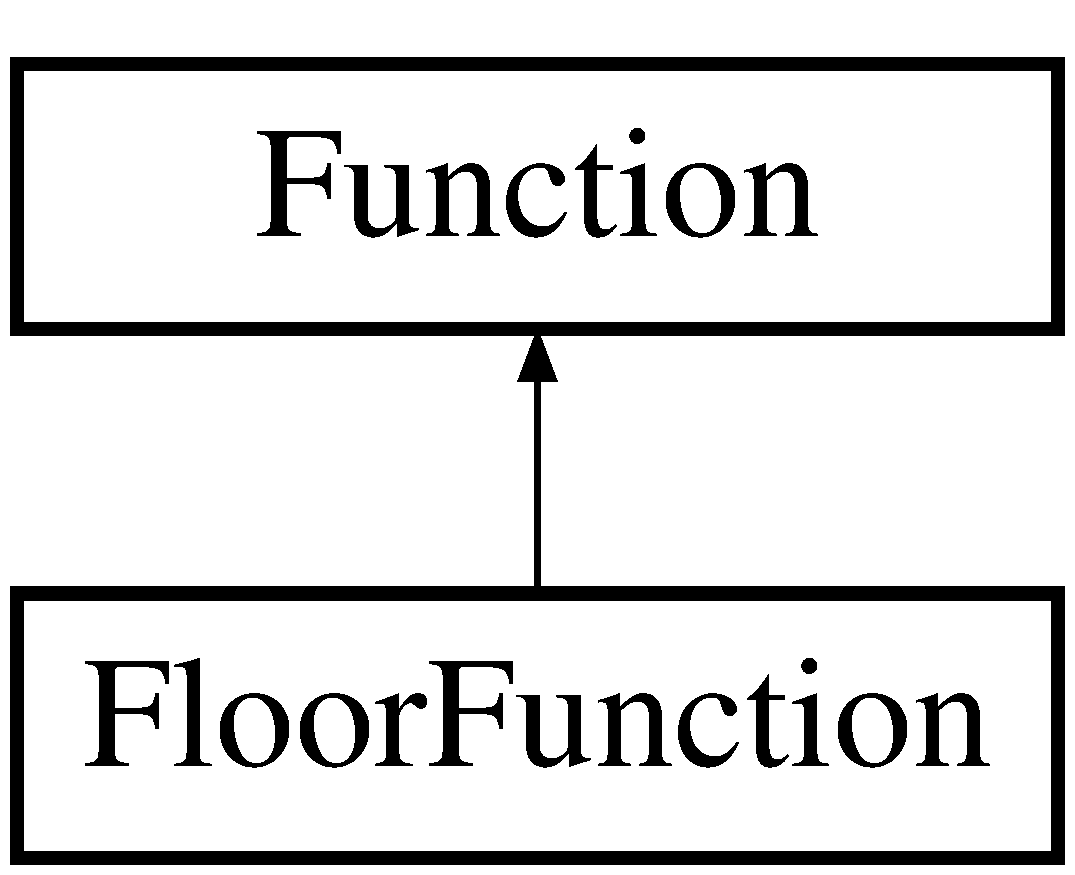
\includegraphics[height=2.000000cm]{class_floor_function}
\end{center}
\end{figure}
\subsection*{Public Member Functions}
\begin{DoxyCompactItemize}
\item 
virtual Decimal \hyperlink{class_floor_function_a3d73d81c614e58fcf8d08cbf2d5c37ab}{value\+At} (Decimal x) const 
\begin{DoxyCompactList}\small\item\em Method to determine the value of \hyperlink{class_floor_function}{Floor\+Function}. \end{DoxyCompactList}\end{DoxyCompactItemize}


\subsection{Detailed Description}
\hyperlink{class_function}{Function} to compute the mathematical floor of the input. 

\subsection{Member Function Documentation}
\hypertarget{class_floor_function_a3d73d81c614e58fcf8d08cbf2d5c37ab}{\index{Floor\+Function@{Floor\+Function}!value\+At@{value\+At}}
\index{value\+At@{value\+At}!Floor\+Function@{Floor\+Function}}
\subsubsection[{value\+At}]{\setlength{\rightskip}{0pt plus 5cm}virtual Decimal Floor\+Function\+::value\+At (
\begin{DoxyParamCaption}
\item[{Decimal}]{x}
\end{DoxyParamCaption}
) const\hspace{0.3cm}{\ttfamily [inline]}, {\ttfamily [virtual]}}}\label{class_floor_function_a3d73d81c614e58fcf8d08cbf2d5c37ab}


Method to determine the value of \hyperlink{class_floor_function}{Floor\+Function}. 

\begin{DoxyReturn}{Returns}
The largest integer less than or equal to {\itshape x}. 
\end{DoxyReturn}


Implements \hyperlink{class_function_a7773feae8f1def0a2d7e479363700816}{Function}.



The documentation for this class was generated from the following file\+:\begin{DoxyCompactItemize}
\item 
Function.\+h\end{DoxyCompactItemize}

\hypertarget{class_function}{\section{Function Class Reference}
\label{class_function}\index{Function@{Function}}
}


A base class for creating mathematical functions plottable by a \hyperlink{class_cartesian_canvas}{Cartesian\+Canvas}.  




{\ttfamily \#include $<$Function.\+h$>$}

Inheritance diagram for Function\+:\begin{figure}[H]
\begin{center}
\leavevmode
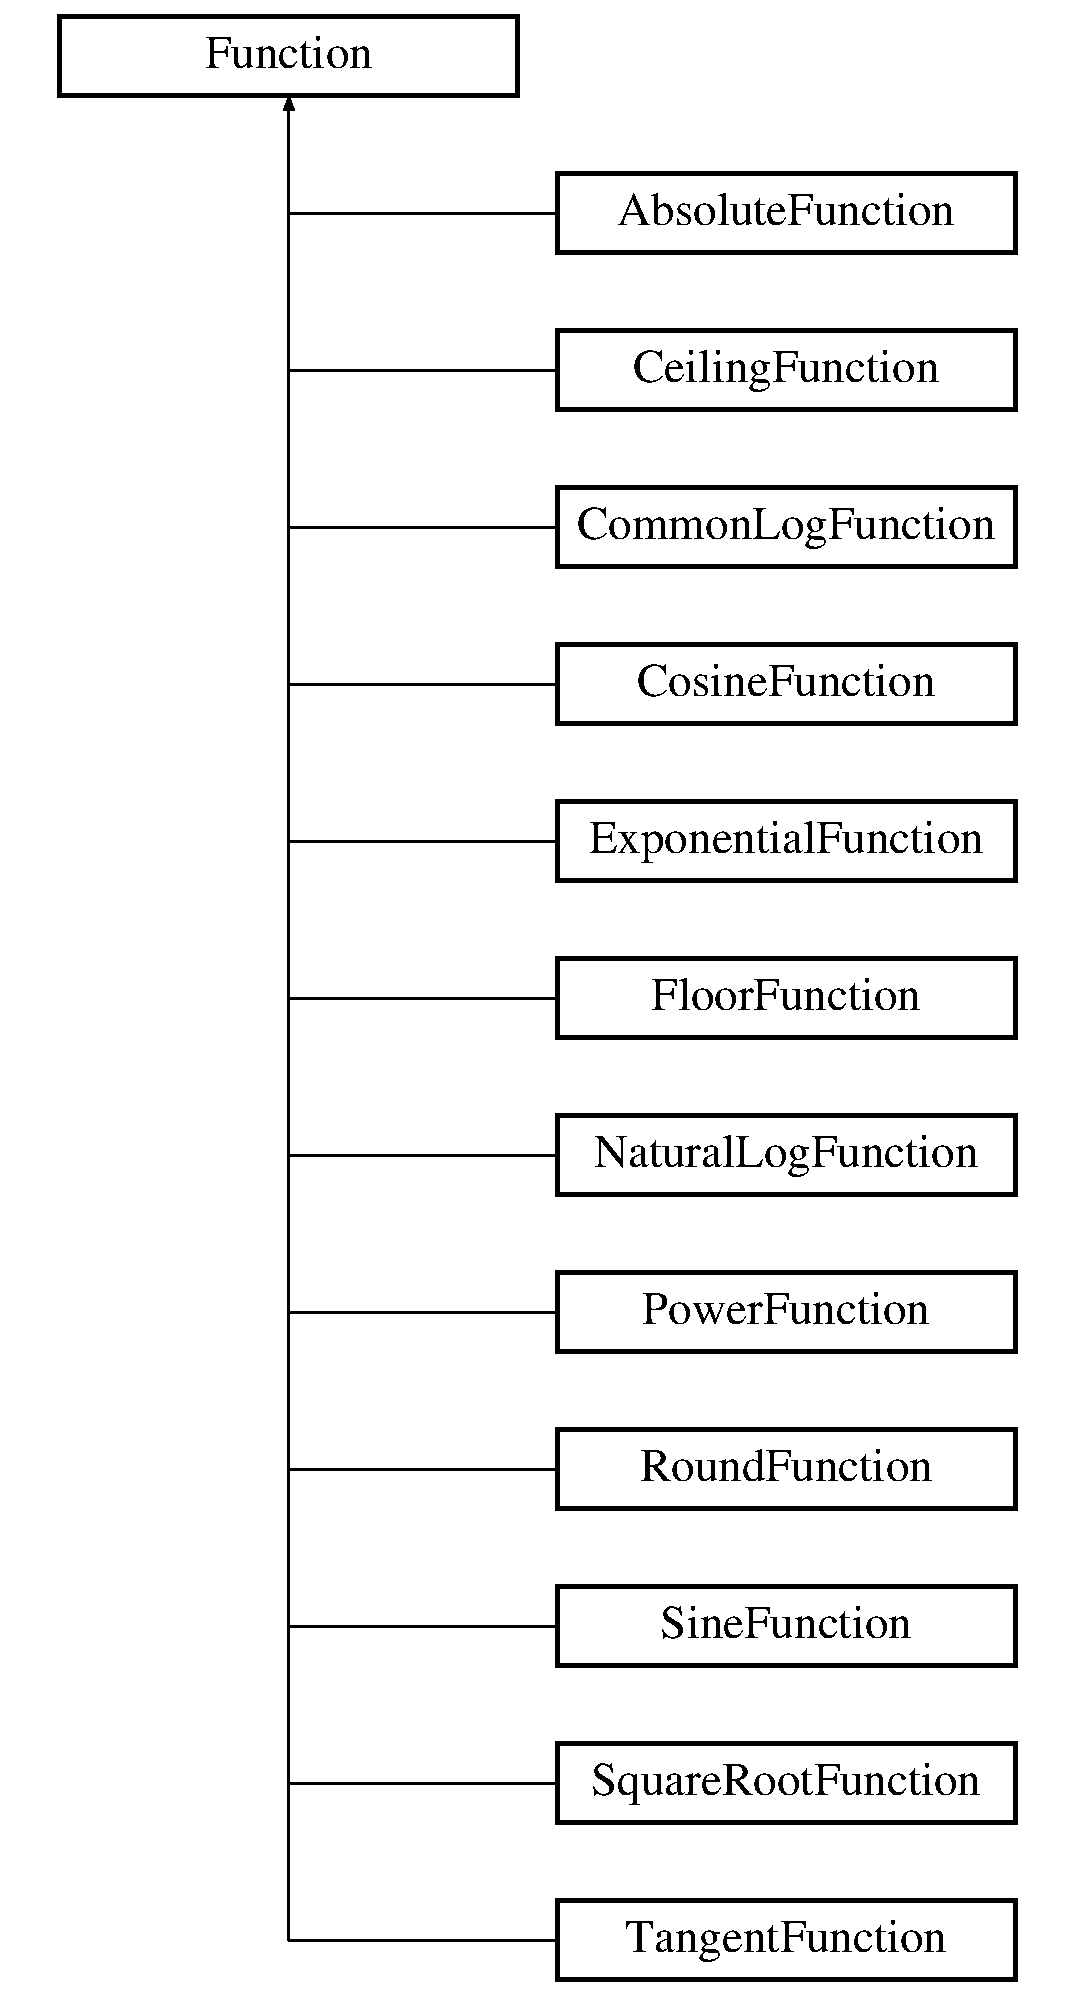
\includegraphics[height=12.000000cm]{class_function}
\end{center}
\end{figure}
\subsection*{Public Member Functions}
\begin{DoxyCompactItemize}
\item 
\hyperlink{class_function_ae206568fd4fd4c885e3ccff76345c4e6}{Function} ()
\begin{DoxyCompactList}\small\item\em Constructs a new \hyperlink{class_function}{Function}. \end{DoxyCompactList}\item 
virtual \hyperlink{class_function_a8697b2e490a4314a7ccbb17aea8ce537}{$\sim$\+Function} ()
\begin{DoxyCompactList}\small\item\em Destructor for the \hyperlink{class_function}{Function} class. \end{DoxyCompactList}\item 
virtual Decimal \hyperlink{class_function_a7773feae8f1def0a2d7e479363700816}{value\+At} (Decimal x) const =0
\begin{DoxyCompactList}\small\item\em Method to determine the value of a \hyperlink{class_function}{Function} subclass. \end{DoxyCompactList}\end{DoxyCompactItemize}


\subsection{Detailed Description}
A base class for creating mathematical functions plottable by a \hyperlink{class_cartesian_canvas}{Cartesian\+Canvas}. 

\hyperlink{class_function}{Function} provides a base class for the creation of mathematical functions. By extending this class and overriding the \hyperlink{class_function_a7773feae8f1def0a2d7e479363700816}{value\+At()} method, users can easily plot the values of their function on a \hyperlink{class_cartesian_canvas}{Cartesian\+Canvas}.  number of prebuilt \hyperlink{class_function}{Function} subclasses are included in the header file for reference. 

\subsection{Constructor \& Destructor Documentation}
\hypertarget{class_function_ae206568fd4fd4c885e3ccff76345c4e6}{\index{Function@{Function}!Function@{Function}}
\index{Function@{Function}!Function@{Function}}
\subsubsection[{Function}]{\setlength{\rightskip}{0pt plus 5cm}Function\+::\+Function (
\begin{DoxyParamCaption}
{}
\end{DoxyParamCaption}
)\hspace{0.3cm}{\ttfamily [inline]}}}\label{class_function_ae206568fd4fd4c885e3ccff76345c4e6}


Constructs a new \hyperlink{class_function}{Function}. 

This is the default constructor for the \hyperlink{class_function}{Function} class \begin{DoxyNote}{Note}
The default constructor for the parent \hyperlink{class_function}{Function} class does absolutely nothing. Any construction should be defined in the subclass. 
\end{DoxyNote}
\hypertarget{class_function_a8697b2e490a4314a7ccbb17aea8ce537}{\index{Function@{Function}!````~Function@{$\sim$\+Function}}
\index{````~Function@{$\sim$\+Function}!Function@{Function}}
\subsubsection[{$\sim$\+Function}]{\setlength{\rightskip}{0pt plus 5cm}virtual Function\+::$\sim$\+Function (
\begin{DoxyParamCaption}
{}
\end{DoxyParamCaption}
)\hspace{0.3cm}{\ttfamily [inline]}, {\ttfamily [virtual]}}}\label{class_function_a8697b2e490a4314a7ccbb17aea8ce537}


Destructor for the \hyperlink{class_function}{Function} class. 

\begin{DoxyNote}{Note}
The default destructor for the parent \hyperlink{class_function}{Function} class does absolutely nothing. Any destruction should be defined in the subclass. 
\end{DoxyNote}


\subsection{Member Function Documentation}
\hypertarget{class_function_a7773feae8f1def0a2d7e479363700816}{\index{Function@{Function}!value\+At@{value\+At}}
\index{value\+At@{value\+At}!Function@{Function}}
\subsubsection[{value\+At}]{\setlength{\rightskip}{0pt plus 5cm}virtual Decimal Function\+::value\+At (
\begin{DoxyParamCaption}
\item[{Decimal}]{x}
\end{DoxyParamCaption}
) const\hspace{0.3cm}{\ttfamily [pure virtual]}}}\label{class_function_a7773feae8f1def0a2d7e479363700816}


Method to determine the value of a \hyperlink{class_function}{Function} subclass. 

This method should be overridden with the actual function you want to computer. 
\begin{DoxyParams}{Parameters}
{\em x} & The input to the function. Assuming your function is F, x will be used to computer F(x). \\
\hline
\end{DoxyParams}
\begin{DoxyReturn}{Returns}
The Decimal value of F(x). 
\end{DoxyReturn}
\begin{DoxyNote}{Note}
This method is abstract and {\bfseries must} be overridden. 
\end{DoxyNote}


Implemented in \hyperlink{class_round_function_aa1d0e06605d9317f4971ffb3b7219825}{Round\+Function}, \hyperlink{class_floor_function_a3d73d81c614e58fcf8d08cbf2d5c37ab}{Floor\+Function}, \hyperlink{class_ceiling_function_a5aac31296f54c9af13acfbe2dc8559d2}{Ceiling\+Function}, \hyperlink{class_common_log_function_a96f716f78cdab4c5458f8372424b52a4}{Common\+Log\+Function}, \hyperlink{class_natural_log_function_af9192cb43f0d62106525dafbdef0b414}{Natural\+Log\+Function}, \hyperlink{class_exponential_function_acb8ed2181be3fa4082a8ff3a61e711a1}{Exponential\+Function}, \hyperlink{class_absolute_function_a10fbd656965076a13b6a58ba908b242f}{Absolute\+Function}, \hyperlink{class_tangent_function_a1353a701417a2be51492d59276e5a5b7}{Tangent\+Function}, \hyperlink{class_cosine_function_a0a0a5067e129d5183b17d4f0bfffd435}{Cosine\+Function}, \hyperlink{class_sine_function_a551d6f4e81a2cdc03c185260a0738a10}{Sine\+Function}, \hyperlink{class_square_root_function_a6044091d737d7bd72325621c2dc56a7a}{Square\+Root\+Function}, and \hyperlink{class_power_function_ad0aa1887b0434963b69a4d51fc725bcc}{Power\+Function}.



Referenced by Cartesian\+Canvas\+::draw\+Function().



The documentation for this class was generated from the following file\+:\begin{DoxyCompactItemize}
\item 
Function.\+h\end{DoxyCompactItemize}

\hypertarget{class_image}{\section{Image Class Reference}
\label{class_image}\index{Image@{Image}}
}


Draw an image to the \hyperlink{class_canvas}{Canvas}.  




{\ttfamily \#include $<$Image.\+h$>$}

Inheritance diagram for Image\+:\begin{figure}[H]
\begin{center}
\leavevmode
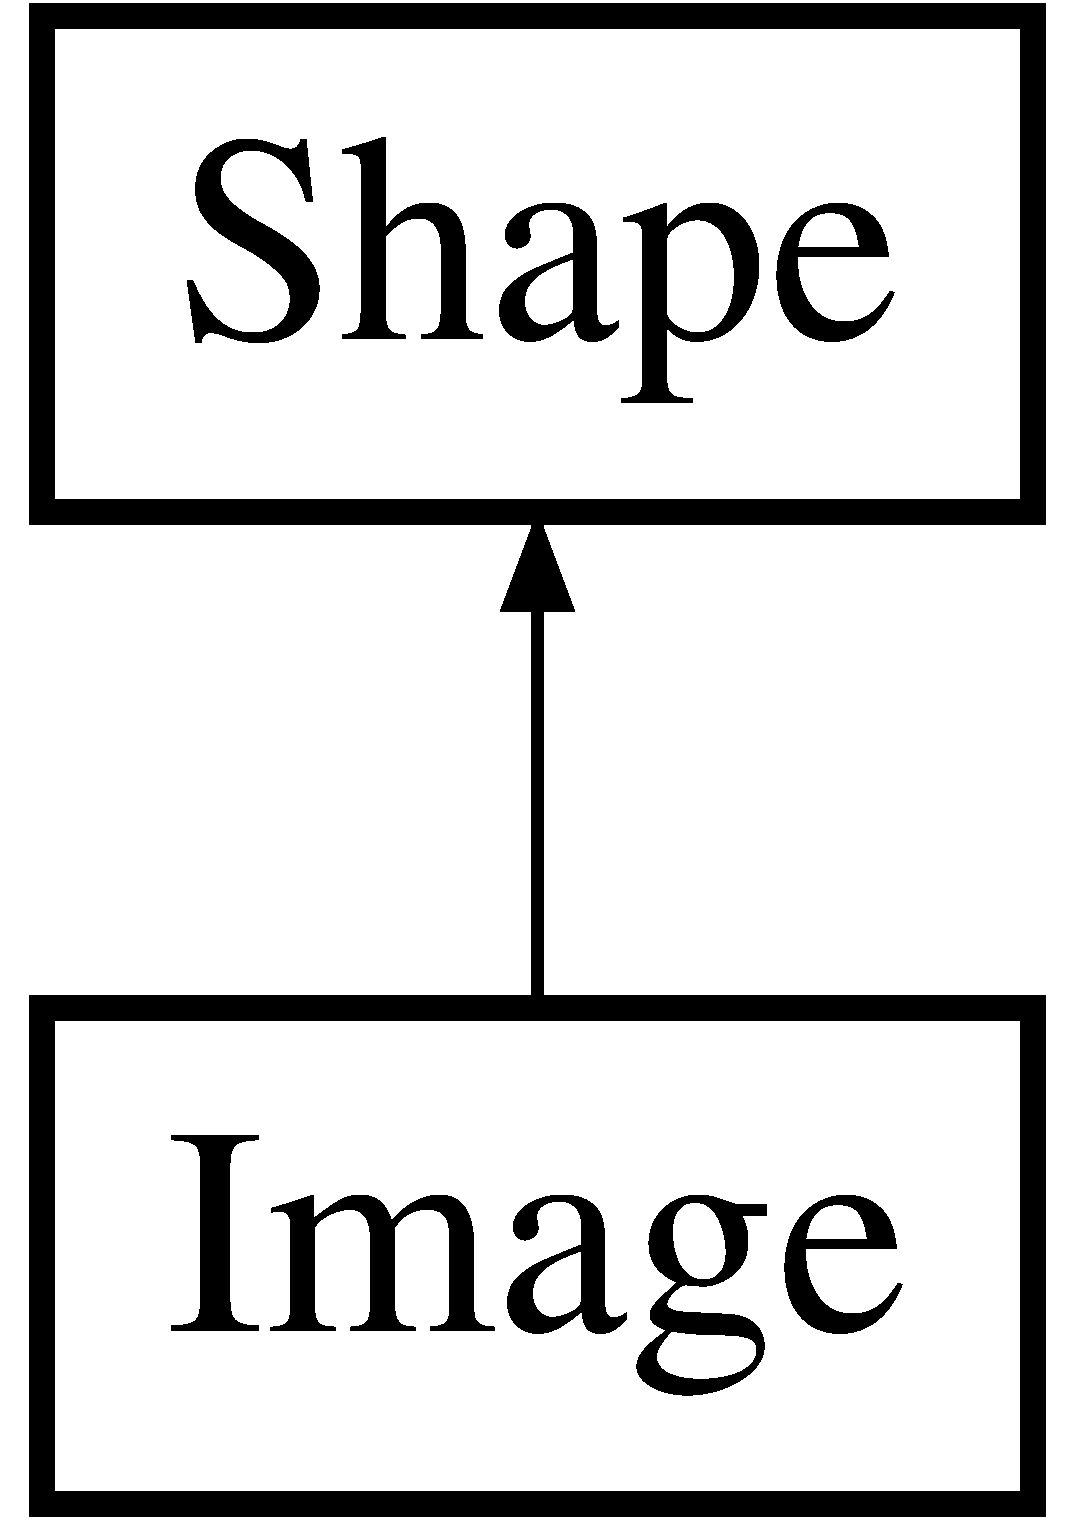
\includegraphics[height=2.000000cm]{class_image}
\end{center}
\end{figure}
\subsection*{Public Member Functions}
\begin{DoxyCompactItemize}
\item 
\hyperlink{class_image_a58510b49ddb40c9bd5d1971d53193a47}{Image} (std\+::string f, Texture\+Handler \&loader, int x, int y, int w, int h, float a)
\begin{DoxyCompactList}\small\item\em Explicitly constructs a new \hyperlink{class_image}{Image}. \end{DoxyCompactList}\item 
void \hyperlink{class_image_ae1e16dcef3072e4e49ec2887a9c1245a}{draw} ()
\begin{DoxyCompactList}\small\item\em Draw the \hyperlink{class_image}{Image}. \end{DoxyCompactList}\end{DoxyCompactItemize}
\subsection*{Additional Inherited Members}


\subsection{Detailed Description}
Draw an image to the \hyperlink{class_canvas}{Canvas}. 

\hyperlink{class_image}{Image} is a class which provides a simple interface for loading and drawing images. The \hyperlink{class_image}{Image} class currently supports files in the .png, .bmp, and .jpg formats. \begin{DoxyNote}{Note}
For the time being, there is no way to measure the size of an image once it's loaded. Therefore, the width and height must be specified manually, and stretching may occur if the inputted dimensions don't match the images actual dimesions. 

Additionally, an Image\+Loader must be passed as an argument. This Image\+Loader is automatically constructed with the \hyperlink{class_canvas}{Canvas} as the private {\itshape loader} variable. At the moment, there is no way to extend \hyperlink{class_canvas_a9c9f7c76fa582510c9fd6bac55d013ab}{Canvas\+::draw\+Image()} function due to this privatization. 
\end{DoxyNote}
\begin{DoxyWarning}{Warning}
Aside from an error message output to stderr, \hyperlink{class_image}{Image} gives no indication if an image failed to load. 
\end{DoxyWarning}


\subsection{Constructor \& Destructor Documentation}
\hypertarget{class_image_a58510b49ddb40c9bd5d1971d53193a47}{\index{Image@{Image}!Image@{Image}}
\index{Image@{Image}!Image@{Image}}
\subsubsection[{Image}]{\setlength{\rightskip}{0pt plus 5cm}Image\+::\+Image (
\begin{DoxyParamCaption}
\item[{std\+::string}]{f, }
\item[{Texture\+Handler \&}]{loader, }
\item[{int}]{x, }
\item[{int}]{y, }
\item[{int}]{w, }
\item[{int}]{h, }
\item[{float}]{a}
\end{DoxyParamCaption}
)}}\label{class_image_a58510b49ddb40c9bd5d1971d53193a47}


Explicitly constructs a new \hyperlink{class_image}{Image}. 

This is the constructor for the \hyperlink{class_image}{Image} class. 
\begin{DoxyParams}{Parameters}
{\em f} & The filename of the image to load. \\
\hline
{\em loader} & A pointer to the Texture\+Handler with which to load the image. \\
\hline
{\em x} & The x coordinate of the left of the \hyperlink{class_image}{Image}. \\
\hline
{\em y} & The y coordinate of the top of the \hyperlink{class_image}{Image}. \\
\hline
{\em w} & The width of the \hyperlink{class_image}{Image}. \\
\hline
{\em h} & The height of the \hyperlink{class_image}{Image}. \\
\hline
{\em a} & The alpha of the \hyperlink{class_image}{Image}. \\
\hline
\end{DoxyParams}
\begin{DoxyReturn}{Returns}
A new \hyperlink{class_image}{Image} drawn with the specified coordinates, dimensions, and transparency. 
\end{DoxyReturn}
\begin{DoxyNote}{Note}
{\bfseries I\+M\+P\+O\+R\+T\+A\+N\+T}\+: In \hyperlink{class_cartesian_canvas}{Cartesian\+Canvas}, {\itshape y} specifies the bottom, not the top, of the image. 
\end{DoxyNote}


\subsection{Member Function Documentation}
\hypertarget{class_image_ae1e16dcef3072e4e49ec2887a9c1245a}{\index{Image@{Image}!draw@{draw}}
\index{draw@{draw}!Image@{Image}}
\subsubsection[{draw}]{\setlength{\rightskip}{0pt plus 5cm}void Image\+::draw (
\begin{DoxyParamCaption}
{}
\end{DoxyParamCaption}
)\hspace{0.3cm}{\ttfamily [virtual]}}}\label{class_image_ae1e16dcef3072e4e49ec2887a9c1245a}


Draw the \hyperlink{class_image}{Image}. 

This function actually draws the \hyperlink{class_image}{Image} to the \hyperlink{class_canvas}{Canvas}. 

Implements \hyperlink{class_shape_afacc5aad8e37308c3ce8fef768199b05}{Shape}.



The documentation for this class was generated from the following files\+:\begin{DoxyCompactItemize}
\item 
Image.\+h\item 
Image.\+cpp\end{DoxyCompactItemize}

\hypertarget{class_line}{\section{Line Class Reference}
\label{class_line}\index{Line@{Line}}
}


Draw a simple line.  




{\ttfamily \#include $<$Line.\+h$>$}

Inheritance diagram for Line\+:\begin{figure}[H]
\begin{center}
\leavevmode
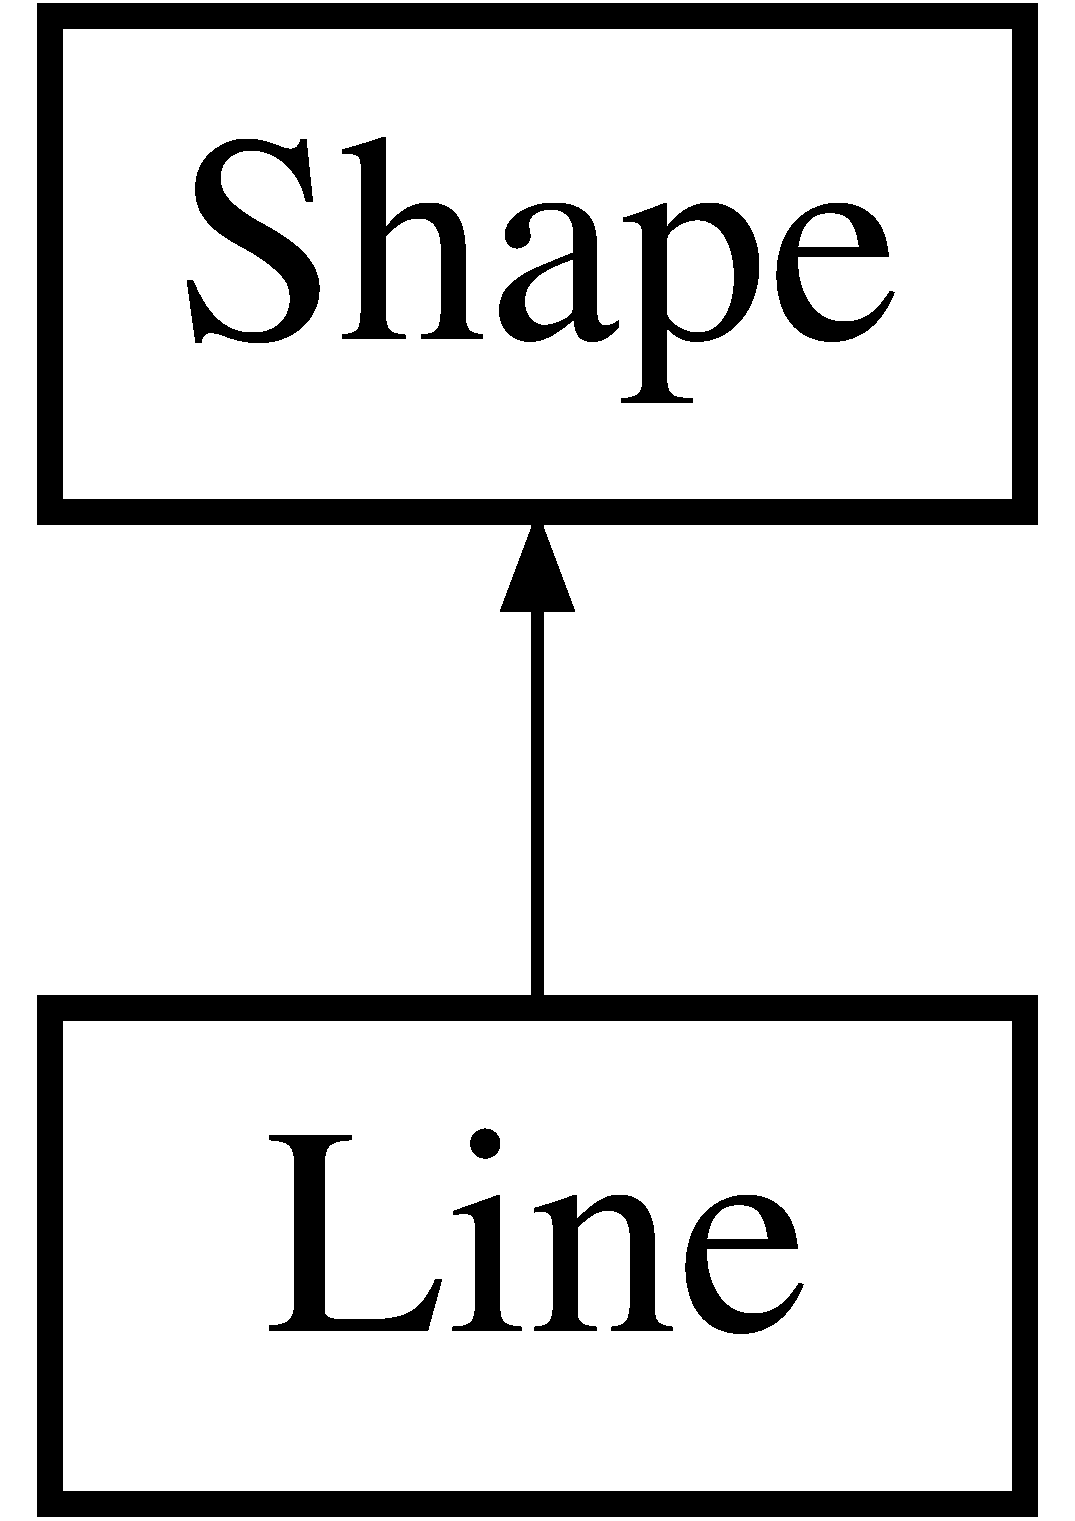
\includegraphics[height=2.000000cm]{class_line}
\end{center}
\end{figure}
\subsection*{Public Member Functions}
\begin{DoxyCompactItemize}
\item 
\hyperlink{class_line_a01fd5349b9a19b2b2ca24a7c7f0e9e9e}{Line} (int x1, int y1, int x2, int y2, const \hyperlink{struct_color_float}{Color\+Float} \&color)
\begin{DoxyCompactList}\small\item\em Explicitly constructs a new \hyperlink{class_line}{Line}. \end{DoxyCompactList}\item 
void \hyperlink{class_line_ab6265993bf5acbc28830181c3e712f10}{draw} ()
\begin{DoxyCompactList}\small\item\em Draw the \hyperlink{class_line}{Line}. \end{DoxyCompactList}\end{DoxyCompactItemize}
\subsection*{Additional Inherited Members}


\subsection{Detailed Description}
Draw a simple line. 

\hyperlink{class_line}{Line} is a class for holding vertex data for a simple line. 

\subsection{Constructor \& Destructor Documentation}
\hypertarget{class_line_a01fd5349b9a19b2b2ca24a7c7f0e9e9e}{\index{Line@{Line}!Line@{Line}}
\index{Line@{Line}!Line@{Line}}
\subsubsection[{Line}]{\setlength{\rightskip}{0pt plus 5cm}Line\+::\+Line (
\begin{DoxyParamCaption}
\item[{int}]{x1, }
\item[{int}]{y1, }
\item[{int}]{x2, }
\item[{int}]{y2, }
\item[{const {\bf Color\+Float} \&}]{color}
\end{DoxyParamCaption}
)}}\label{class_line_a01fd5349b9a19b2b2ca24a7c7f0e9e9e}


Explicitly constructs a new \hyperlink{class_line}{Line}. 

This is the constructor for the \hyperlink{class_line}{Line} class. 
\begin{DoxyParams}{Parameters}
{\em x1} & The x coordinate of the first endpoint. \\
\hline
{\em y1} & The y coordinate of the first endpoint. \\
\hline
{\em x2} & The x coordinate of the second endpoint. \\
\hline
{\em y2} & The y coordinate of the second endpoint. \\
\hline
{\em color} & The color of the \hyperlink{class_line}{Line}. \\
\hline
\end{DoxyParams}
\begin{DoxyReturn}{Returns}
A new \hyperlink{class_line}{Line} with the specified endpoints and color. 
\end{DoxyReturn}


\subsection{Member Function Documentation}
\hypertarget{class_line_ab6265993bf5acbc28830181c3e712f10}{\index{Line@{Line}!draw@{draw}}
\index{draw@{draw}!Line@{Line}}
\subsubsection[{draw}]{\setlength{\rightskip}{0pt plus 5cm}void Line\+::draw (
\begin{DoxyParamCaption}
{}
\end{DoxyParamCaption}
)\hspace{0.3cm}{\ttfamily [virtual]}}}\label{class_line_ab6265993bf5acbc28830181c3e712f10}


Draw the \hyperlink{class_line}{Line}. 

This function actually draws the \hyperlink{class_line}{Line} to the \hyperlink{class_canvas}{Canvas}. 

Implements \hyperlink{class_shape_afacc5aad8e37308c3ce8fef768199b05}{Shape}.



The documentation for this class was generated from the following files\+:\begin{DoxyCompactItemize}
\item 
Line.\+h\item 
Line.\+cpp\end{DoxyCompactItemize}

\hypertarget{class_natural_log_function}{\section{Natural\+Log\+Function Class Reference}
\label{class_natural_log_function}\index{Natural\+Log\+Function@{Natural\+Log\+Function}}
}


\hyperlink{class_function}{Function} to compute the natural log of the input.  




{\ttfamily \#include $<$Function.\+h$>$}

Inheritance diagram for Natural\+Log\+Function\+:\begin{figure}[H]
\begin{center}
\leavevmode
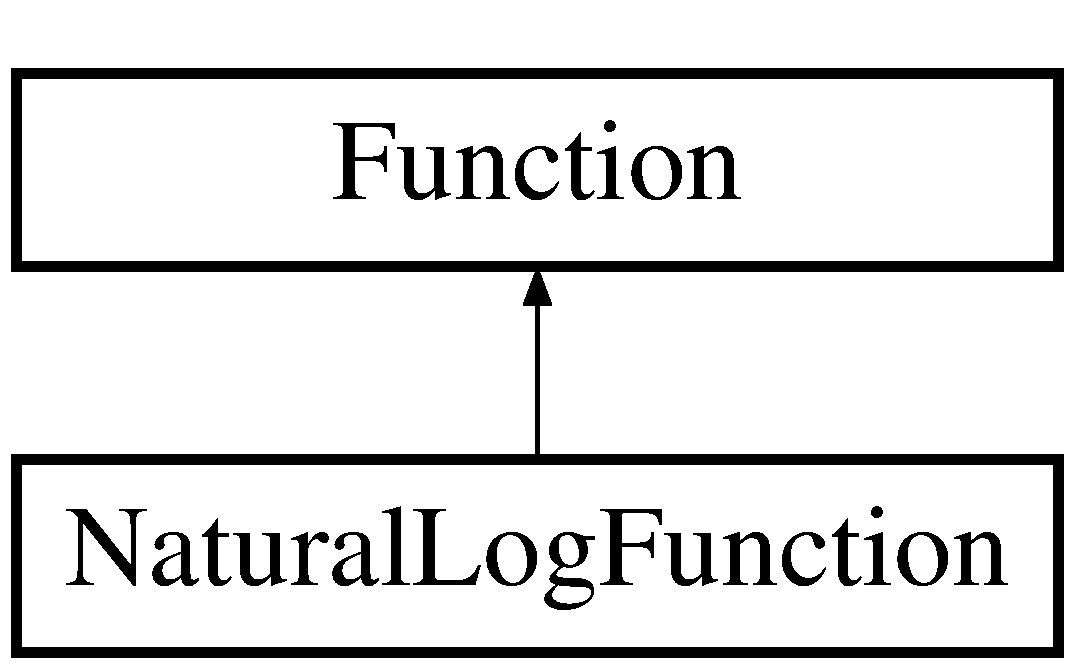
\includegraphics[height=2.000000cm]{class_natural_log_function}
\end{center}
\end{figure}
\subsection*{Public Member Functions}
\begin{DoxyCompactItemize}
\item 
virtual Decimal \hyperlink{class_natural_log_function_af9192cb43f0d62106525dafbdef0b414}{value\+At} (Decimal x) const 
\begin{DoxyCompactList}\small\item\em Method to determine the value of \hyperlink{class_natural_log_function}{Natural\+Log\+Function}. \end{DoxyCompactList}\end{DoxyCompactItemize}


\subsection{Detailed Description}
\hyperlink{class_function}{Function} to compute the natural log of the input. 

\subsection{Member Function Documentation}
\hypertarget{class_natural_log_function_af9192cb43f0d62106525dafbdef0b414}{\index{Natural\+Log\+Function@{Natural\+Log\+Function}!value\+At@{value\+At}}
\index{value\+At@{value\+At}!Natural\+Log\+Function@{Natural\+Log\+Function}}
\subsubsection[{value\+At}]{\setlength{\rightskip}{0pt plus 5cm}virtual Decimal Natural\+Log\+Function\+::value\+At (
\begin{DoxyParamCaption}
\item[{Decimal}]{x}
\end{DoxyParamCaption}
) const\hspace{0.3cm}{\ttfamily [inline]}, {\ttfamily [virtual]}}}\label{class_natural_log_function_af9192cb43f0d62106525dafbdef0b414}


Method to determine the value of \hyperlink{class_natural_log_function}{Natural\+Log\+Function}. 

\begin{DoxyReturn}{Returns}
The natural log of {\itshape x}. 
\end{DoxyReturn}


Implements \hyperlink{class_function_a7773feae8f1def0a2d7e479363700816}{Function}.



The documentation for this class was generated from the following file\+:\begin{DoxyCompactItemize}
\item 
Function.\+h\end{DoxyCompactItemize}

\hypertarget{class_polyline}{\section{Polyline Class Reference}
\label{class_polyline}\index{Polyline@{Polyline}}
}


Draw multiple lines chained together.  




{\ttfamily \#include $<$Polyline.\+h$>$}

Inheritance diagram for Polyline\+:\begin{figure}[H]
\begin{center}
\leavevmode
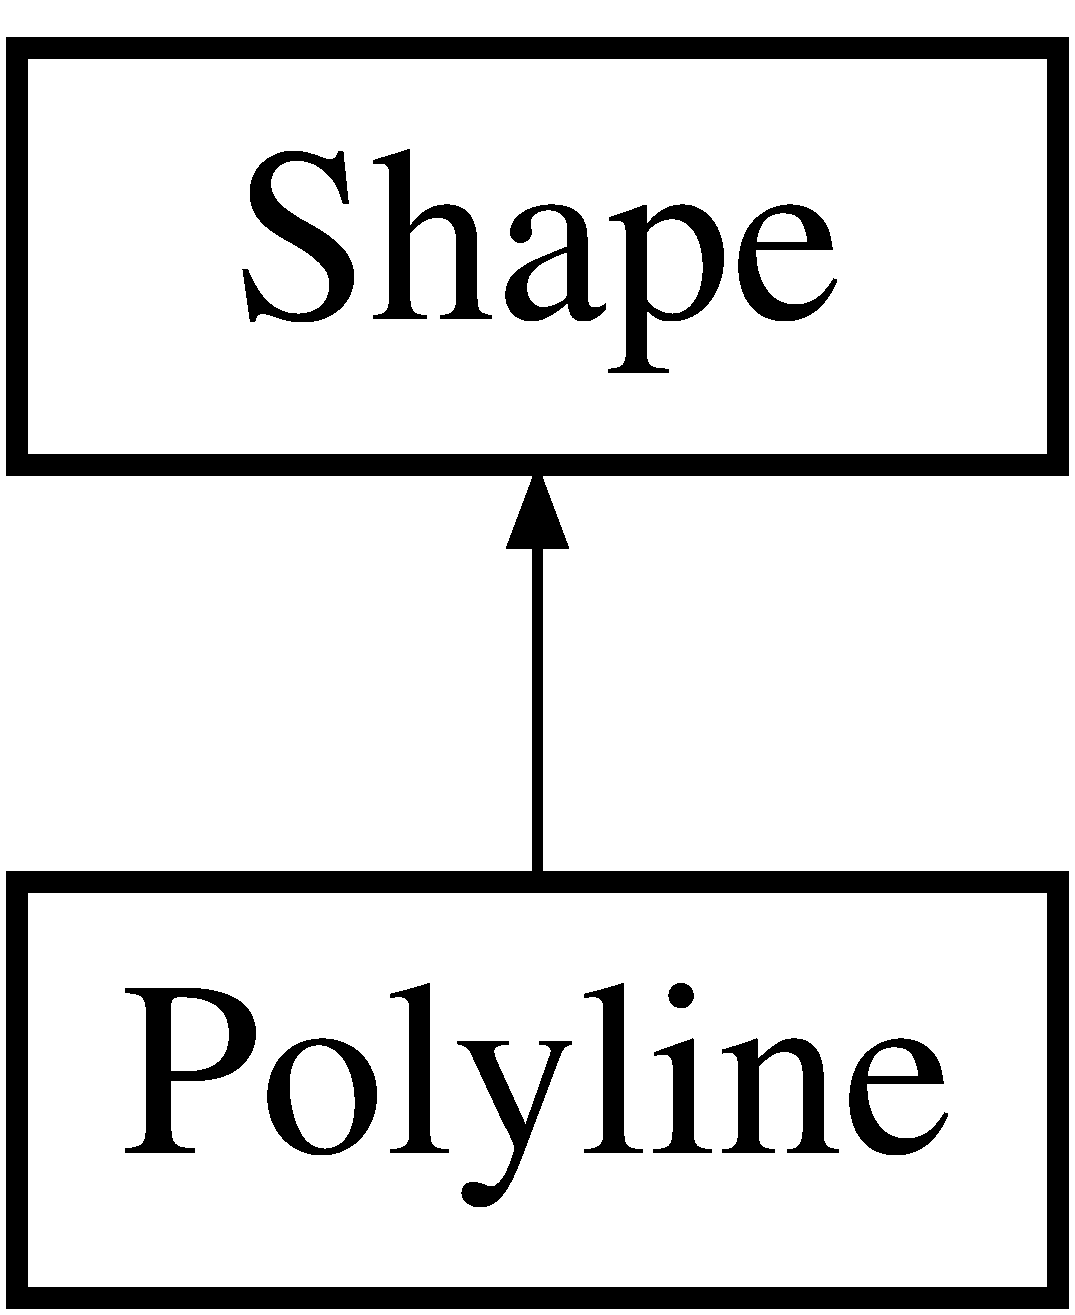
\includegraphics[height=2.000000cm]{class_polyline}
\end{center}
\end{figure}
\subsection*{Public Member Functions}
\begin{DoxyCompactItemize}
\item 
\hyperlink{class_polyline_a01c3f4e90326a346cd5f70c95d107cb9}{Polyline} (int v)
\begin{DoxyCompactList}\small\item\em Explicitly constructor a new \hyperlink{class_polyline}{Polyline}. \end{DoxyCompactList}\item 
void \hyperlink{class_polyline_ac025e62a56822d0f2747e8b08614ee85}{add\+Next\+Vertex} (int x, int y, const \hyperlink{struct_color_float}{Color\+Float} \&color=B\+L\+A\+C\+K)
\begin{DoxyCompactList}\small\item\em Add another vertex to the \hyperlink{class_polyline}{Polyline}. \end{DoxyCompactList}\item 
void \hyperlink{class_polyline_a21ea8147cb2a0d8d9b61af7b62520395}{draw} ()
\begin{DoxyCompactList}\small\item\em Draw the \hyperlink{class_polyline}{Polyline}. \end{DoxyCompactList}\end{DoxyCompactItemize}
\subsection*{Additional Inherited Members}


\subsection{Detailed Description}
Draw multiple lines chained together. 

\hyperlink{class_polyline}{Polyline} is a class for holding vertex data for multiple lines whose endpoints are connected.

This method is optimized for long lists and offers a marked improvement over drawing individual \hyperlink{class_line}{Line} instances. \begin{DoxyNote}{Note}
The add\+Vertex() method must be called the same number of times as specified in the constructor. 

Calling add\+Vertex() after all vertices have been added will do nothing. 

Calling \hyperlink{class_polyline_a21ea8147cb2a0d8d9b61af7b62520395}{draw()} before all vertices have been added will do nothing. 
\end{DoxyNote}


\subsection{Constructor \& Destructor Documentation}
\hypertarget{class_polyline_a01c3f4e90326a346cd5f70c95d107cb9}{\index{Polyline@{Polyline}!Polyline@{Polyline}}
\index{Polyline@{Polyline}!Polyline@{Polyline}}
\subsubsection[{Polyline}]{\setlength{\rightskip}{0pt plus 5cm}Polyline\+::\+Polyline (
\begin{DoxyParamCaption}
\item[{int}]{v}
\end{DoxyParamCaption}
)}}\label{class_polyline_a01c3f4e90326a346cd5f70c95d107cb9}


Explicitly constructor a new \hyperlink{class_polyline}{Polyline}. 


\begin{DoxyParams}{Parameters}
{\em v,the} & number of vertices the complete \hyperlink{class_polyline}{Polyline} will have. \\
\hline
\end{DoxyParams}
\begin{DoxyReturn}{Returns}
a new \hyperlink{class_polyline}{Polyline} with a buffer for storing the specified numbered of vertices. 
\end{DoxyReturn}


\subsection{Member Function Documentation}
\hypertarget{class_polyline_ac025e62a56822d0f2747e8b08614ee85}{\index{Polyline@{Polyline}!add\+Next\+Vertex@{add\+Next\+Vertex}}
\index{add\+Next\+Vertex@{add\+Next\+Vertex}!Polyline@{Polyline}}
\subsubsection[{add\+Next\+Vertex}]{\setlength{\rightskip}{0pt plus 5cm}void Polyline\+::add\+Next\+Vertex (
\begin{DoxyParamCaption}
\item[{int}]{x, }
\item[{int}]{y, }
\item[{const {\bf Color\+Float} \&}]{color = {\ttfamily BLACK}}
\end{DoxyParamCaption}
)}}\label{class_polyline_ac025e62a56822d0f2747e8b08614ee85}


Add another vertex to the \hyperlink{class_polyline}{Polyline}. 

This function initalizes the next vertex in the \hyperlink{class_polyline}{Polyline} and adds it to the \hyperlink{class_polyline}{Polyline}'s buffer. 
\begin{DoxyParams}{Parameters}
{\em x} & The x position of the vertex. \\
\hline
{\em y} & The y position of the vertex. \\
\hline
{\em color} & The color of the vertex. \\
\hline
\end{DoxyParams}
\begin{DoxyNote}{Note}
This function does nothing if the vertex buffer is already full. 
\end{DoxyNote}


Referenced by Canvas\+::draw\+Circle(), Canvas\+::draw\+Colored\+Polygon(), Cartesian\+Canvas\+::draw\+Function(), Canvas\+::draw\+Rectangle(), and Canvas\+::draw\+Triangle().

\hypertarget{class_polyline_a21ea8147cb2a0d8d9b61af7b62520395}{\index{Polyline@{Polyline}!draw@{draw}}
\index{draw@{draw}!Polyline@{Polyline}}
\subsubsection[{draw}]{\setlength{\rightskip}{0pt plus 5cm}void Polyline\+::draw (
\begin{DoxyParamCaption}
{}
\end{DoxyParamCaption}
)\hspace{0.3cm}{\ttfamily [virtual]}}}\label{class_polyline_a21ea8147cb2a0d8d9b61af7b62520395}


Draw the \hyperlink{class_polyline}{Polyline}. 

This function actually draws the \hyperlink{class_polyline}{Polyline} to the \hyperlink{class_canvas}{Canvas}. \begin{DoxyNote}{Note}
This function does nothing if the vertex buffer is not yet full. 
\end{DoxyNote}


Implements \hyperlink{class_shape_afacc5aad8e37308c3ce8fef768199b05}{Shape}.



The documentation for this class was generated from the following files\+:\begin{DoxyCompactItemize}
\item 
Polyline.\+h\item 
Polyline.\+cpp\end{DoxyCompactItemize}

\hypertarget{class_power_function}{\section{Power\+Function Class Reference}
\label{class_power_function}\index{Power\+Function@{Power\+Function}}
}


\hyperlink{class_function}{Function} to compute the input raised to a specified power.  




{\ttfamily \#include $<$Function.\+h$>$}

Inheritance diagram for Power\+Function\+:\begin{figure}[H]
\begin{center}
\leavevmode
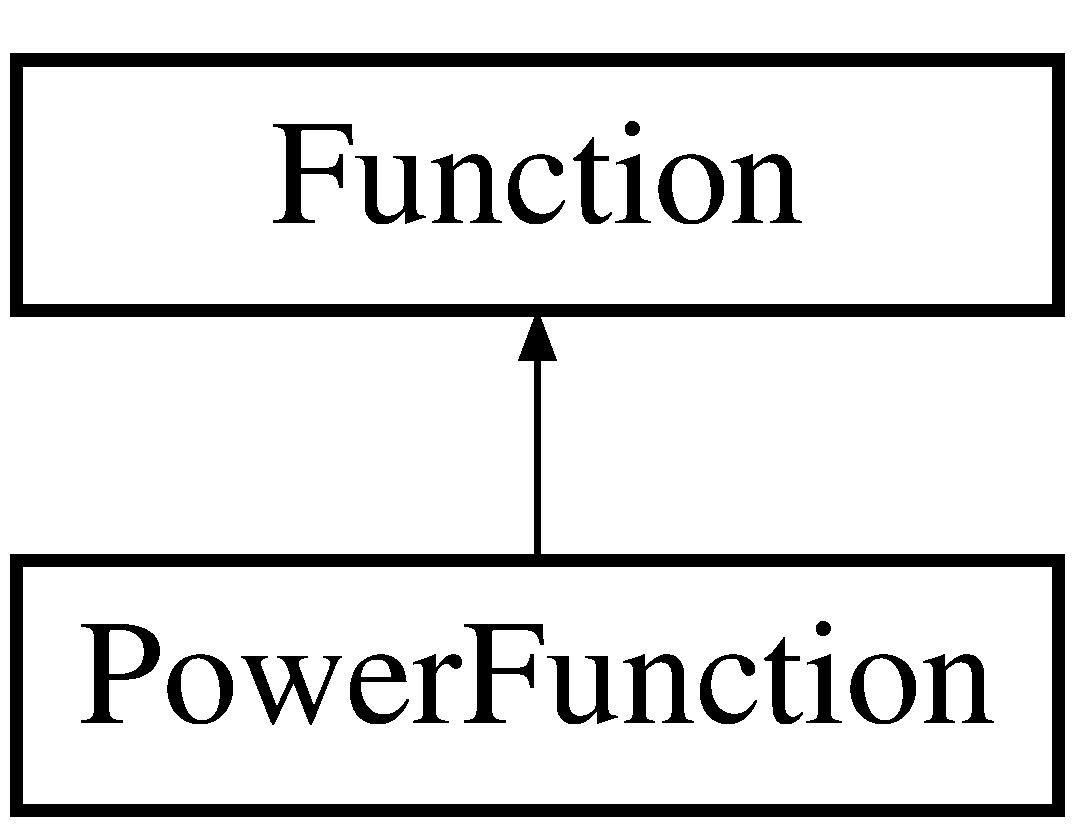
\includegraphics[height=2.000000cm]{class_power_function}
\end{center}
\end{figure}
\subsection*{Public Member Functions}
\begin{DoxyCompactItemize}
\item 
\hyperlink{class_power_function_ae7b11ee2001d49cd47d0d5983f6742a7}{Power\+Function} (Decimal a)
\begin{DoxyCompactList}\small\item\em Constructs a new \hyperlink{class_power_function}{Power\+Function}. \end{DoxyCompactList}\item 
virtual Decimal \hyperlink{class_power_function_ad0aa1887b0434963b69a4d51fc725bcc}{value\+At} (Decimal x) const 
\begin{DoxyCompactList}\small\item\em Method to determine the value of \hyperlink{class_power_function}{Power\+Function}. \end{DoxyCompactList}\end{DoxyCompactItemize}


\subsection{Detailed Description}
\hyperlink{class_function}{Function} to compute the input raised to a specified power. 

\subsection{Constructor \& Destructor Documentation}
\hypertarget{class_power_function_ae7b11ee2001d49cd47d0d5983f6742a7}{\index{Power\+Function@{Power\+Function}!Power\+Function@{Power\+Function}}
\index{Power\+Function@{Power\+Function}!Power\+Function@{Power\+Function}}
\subsubsection[{Power\+Function}]{\setlength{\rightskip}{0pt plus 5cm}Power\+Function\+::\+Power\+Function (
\begin{DoxyParamCaption}
\item[{Decimal}]{a}
\end{DoxyParamCaption}
)\hspace{0.3cm}{\ttfamily [inline]}}}\label{class_power_function_ae7b11ee2001d49cd47d0d5983f6742a7}


Constructs a new \hyperlink{class_power_function}{Power\+Function}. 


\begin{DoxyParams}{Parameters}
{\em a} & The power to which the input is raised. \\
\hline
\end{DoxyParams}


\subsection{Member Function Documentation}
\hypertarget{class_power_function_ad0aa1887b0434963b69a4d51fc725bcc}{\index{Power\+Function@{Power\+Function}!value\+At@{value\+At}}
\index{value\+At@{value\+At}!Power\+Function@{Power\+Function}}
\subsubsection[{value\+At}]{\setlength{\rightskip}{0pt plus 5cm}virtual Decimal Power\+Function\+::value\+At (
\begin{DoxyParamCaption}
\item[{Decimal}]{x}
\end{DoxyParamCaption}
) const\hspace{0.3cm}{\ttfamily [inline]}, {\ttfamily [virtual]}}}\label{class_power_function_ad0aa1887b0434963b69a4d51fc725bcc}


Method to determine the value of \hyperlink{class_power_function}{Power\+Function}. 


\begin{DoxyParams}{Parameters}
{\em x} & The input to the function. \\
\hline
\end{DoxyParams}
\begin{DoxyReturn}{Returns}
{\itshape x} raised to the $\ast$a$\ast$th power. 
\end{DoxyReturn}


Implements \hyperlink{class_function_a7773feae8f1def0a2d7e479363700816}{Function}.



The documentation for this class was generated from the following file\+:\begin{DoxyCompactItemize}
\item 
Function.\+h\end{DoxyCompactItemize}

\hypertarget{class_rectangle}{\section{Rectangle Class Reference}
\label{class_rectangle}\index{Rectangle@{Rectangle}}
}


Draw a simple \hyperlink{class_rectangle}{Rectangle}.  




{\ttfamily \#include $<$Rectangle.\+h$>$}

Inheritance diagram for Rectangle\+:\begin{figure}[H]
\begin{center}
\leavevmode
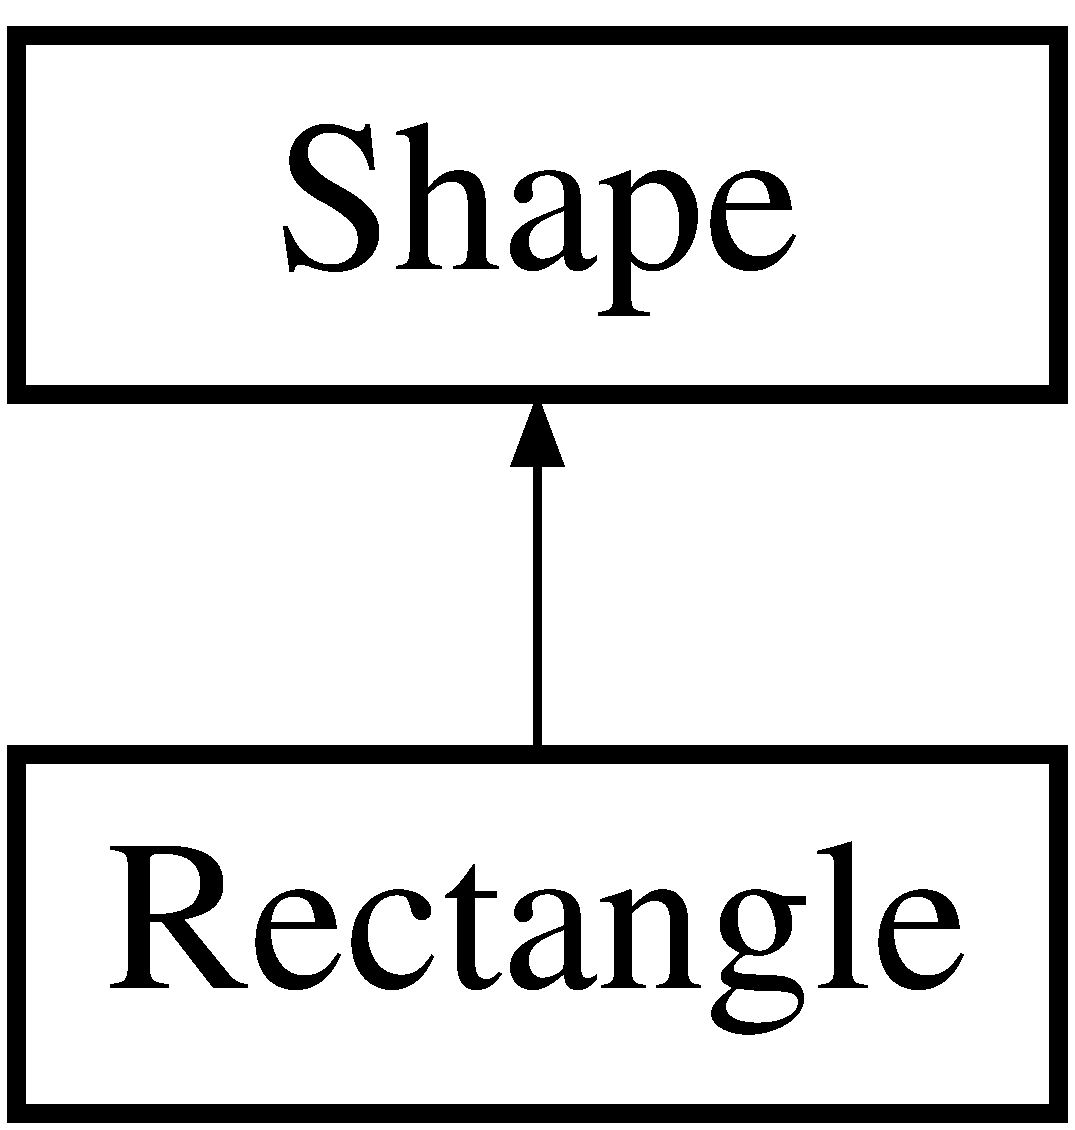
\includegraphics[height=2.000000cm]{class_rectangle}
\end{center}
\end{figure}
\subsection*{Public Member Functions}
\begin{DoxyCompactItemize}
\item 
\hyperlink{class_rectangle_aefa6120fd93fe488322280e9abfafde4}{Rectangle} (int x, int y, int w, int h, const \hyperlink{struct_color_float}{Color\+Float} \&color)
\begin{DoxyCompactList}\small\item\em Explicitly construct a \hyperlink{class_rectangle}{Rectangle}. \end{DoxyCompactList}\item 
void \hyperlink{class_rectangle_ac895c67f1d6337e3b4f72663b17dd299}{draw} ()
\begin{DoxyCompactList}\small\item\em Draw the \hyperlink{class_rectangle}{Rectangle}. \end{DoxyCompactList}\end{DoxyCompactItemize}
\subsection*{Additional Inherited Members}


\subsection{Detailed Description}
Draw a simple \hyperlink{class_rectangle}{Rectangle}. 

\hyperlink{class_rectangle}{Rectangle} is a class for holding vertex data for a simple rectangle. 

\subsection{Constructor \& Destructor Documentation}
\hypertarget{class_rectangle_aefa6120fd93fe488322280e9abfafde4}{\index{Rectangle@{Rectangle}!Rectangle@{Rectangle}}
\index{Rectangle@{Rectangle}!Rectangle@{Rectangle}}
\subsubsection[{Rectangle}]{\setlength{\rightskip}{0pt plus 5cm}Rectangle\+::\+Rectangle (
\begin{DoxyParamCaption}
\item[{int}]{x, }
\item[{int}]{y, }
\item[{int}]{w, }
\item[{int}]{h, }
\item[{const {\bf Color\+Float} \&}]{color}
\end{DoxyParamCaption}
)}}\label{class_rectangle_aefa6120fd93fe488322280e9abfafde4}


Explicitly construct a \hyperlink{class_rectangle}{Rectangle}. 

This is the constructor for the \hyperlink{class_rectangle}{Rectangle} class. 
\begin{DoxyParams}{Parameters}
{\em x} & The x coordinate of the \hyperlink{class_rectangle}{Rectangle}'s left edge. \\
\hline
{\em y} & The y coordinate of the \hyperlink{class_rectangle}{Rectangle}'s top edge. \\
\hline
{\em w} & The width of the \hyperlink{class_rectangle}{Rectangle}. \\
\hline
{\em h} & The height of the \hyperlink{class_rectangle}{Rectangle}. \\
\hline
{\em color} & The color of the \hyperlink{class_rectangle}{Rectangle}. \\
\hline
\end{DoxyParams}
\begin{DoxyReturn}{Returns}
a new \hyperlink{class_rectangle}{Rectangle} with the specified top left corner, dimensions, and color. 
\end{DoxyReturn}


\subsection{Member Function Documentation}
\hypertarget{class_rectangle_ac895c67f1d6337e3b4f72663b17dd299}{\index{Rectangle@{Rectangle}!draw@{draw}}
\index{draw@{draw}!Rectangle@{Rectangle}}
\subsubsection[{draw}]{\setlength{\rightskip}{0pt plus 5cm}void Rectangle\+::draw (
\begin{DoxyParamCaption}
{}
\end{DoxyParamCaption}
)\hspace{0.3cm}{\ttfamily [virtual]}}}\label{class_rectangle_ac895c67f1d6337e3b4f72663b17dd299}


Draw the \hyperlink{class_rectangle}{Rectangle}. 

This function actually draws the \hyperlink{class_rectangle}{Rectangle} to the \hyperlink{class_canvas}{Canvas}. 

Implements \hyperlink{class_shape_afacc5aad8e37308c3ce8fef768199b05}{Shape}.



The documentation for this class was generated from the following files\+:\begin{DoxyCompactItemize}
\item 
Rectangle.\+h\item 
Rectangle.\+cpp\end{DoxyCompactItemize}

\hypertarget{class_round_function}{\section{Round\+Function Class Reference}
\label{class_round_function}\index{Round\+Function@{Round\+Function}}
}


\hyperlink{class_function}{Function} to round the input to the nearest integer number.  




{\ttfamily \#include $<$Function.\+h$>$}

Inheritance diagram for Round\+Function\+:\begin{figure}[H]
\begin{center}
\leavevmode
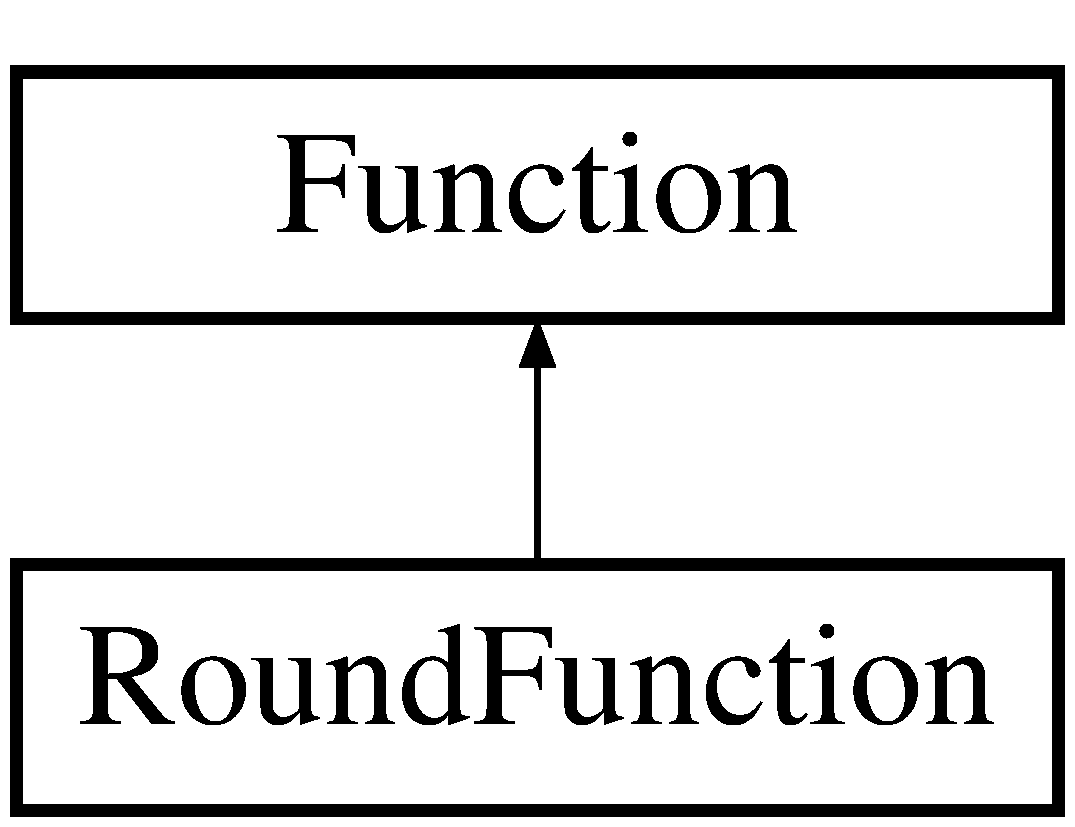
\includegraphics[height=2.000000cm]{class_round_function}
\end{center}
\end{figure}
\subsection*{Public Member Functions}
\begin{DoxyCompactItemize}
\item 
virtual Decimal \hyperlink{class_round_function_aa1d0e06605d9317f4971ffb3b7219825}{value\+At} (Decimal x) const 
\begin{DoxyCompactList}\small\item\em Method to determine the value of \hyperlink{class_round_function}{Round\+Function}. \end{DoxyCompactList}\end{DoxyCompactItemize}


\subsection{Detailed Description}
\hyperlink{class_function}{Function} to round the input to the nearest integer number. 

\subsection{Member Function Documentation}
\hypertarget{class_round_function_aa1d0e06605d9317f4971ffb3b7219825}{\index{Round\+Function@{Round\+Function}!value\+At@{value\+At}}
\index{value\+At@{value\+At}!Round\+Function@{Round\+Function}}
\subsubsection[{value\+At}]{\setlength{\rightskip}{0pt plus 5cm}virtual Decimal Round\+Function\+::value\+At (
\begin{DoxyParamCaption}
\item[{Decimal}]{x}
\end{DoxyParamCaption}
) const\hspace{0.3cm}{\ttfamily [inline]}, {\ttfamily [virtual]}}}\label{class_round_function_aa1d0e06605d9317f4971ffb3b7219825}


Method to determine the value of \hyperlink{class_round_function}{Round\+Function}. 

\begin{DoxyReturn}{Returns}
The closest integer to {\itshape x}. 
\end{DoxyReturn}


Implements \hyperlink{class_function_a7773feae8f1def0a2d7e479363700816}{Function}.



The documentation for this class was generated from the following file\+:\begin{DoxyCompactItemize}
\item 
Function.\+h\end{DoxyCompactItemize}

\hypertarget{class_shape}{\section{Shape Class Reference}
\label{class_shape}\index{Shape@{Shape}}
}


A class for drawing shapes onto a \hyperlink{class_canvas}{Canvas} or \hyperlink{class_cartesian_canvas}{Cartesian\+Canvas}.  




{\ttfamily \#include $<$Shape.\+h$>$}

Inheritance diagram for Shape\+:\begin{figure}[H]
\begin{center}
\leavevmode
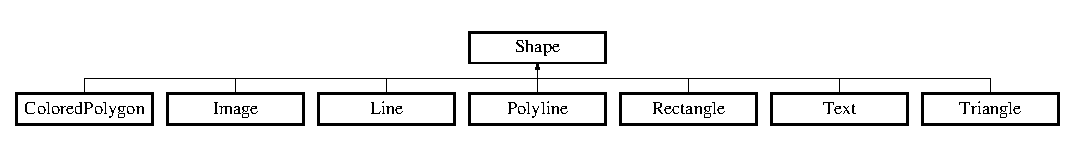
\includegraphics[height=1.441442cm]{class_shape}
\end{center}
\end{figure}
\subsection*{Public Member Functions}
\begin{DoxyCompactItemize}
\item 
\hyperlink{class_shape_aaa8d87171e65e0d8ba3c5459978992a7}{Shape} ()
\begin{DoxyCompactList}\small\item\em Constructs a new \hyperlink{class_shape}{Shape}. \end{DoxyCompactList}\item 
virtual \hyperlink{class_shape_ac3b9fc48965274893f25b18aa14ba665}{$\sim$\+Shape} ()
\begin{DoxyCompactList}\small\item\em Destructor for the \hyperlink{class_shape}{Shape}. \end{DoxyCompactList}\item 
virtual void \hyperlink{class_shape_afacc5aad8e37308c3ce8fef768199b05}{draw} ()=0
\begin{DoxyCompactList}\small\item\em Actually draws the shape to the \hyperlink{class_canvas}{Canvas}. \end{DoxyCompactList}\item 
\hypertarget{class_shape_a8ccc804d7528af16e3a14017b52dbe58}{bool \hyperlink{class_shape_a8ccc804d7528af16e3a14017b52dbe58}{get\+Is\+Textured} ()}\label{class_shape_a8ccc804d7528af16e3a14017b52dbe58}

\begin{DoxyCompactList}\small\item\em Accessor for {\itshape is\+Textured}. \end{DoxyCompactList}\end{DoxyCompactItemize}
\subsection*{Protected Attributes}
\begin{DoxyCompactItemize}
\item 
\hypertarget{class_shape_ad21644e3f39633feb48ad5b822301495}{bool {\bfseries is\+Textured}}\label{class_shape_ad21644e3f39633feb48ad5b822301495}

\end{DoxyCompactItemize}


\subsection{Detailed Description}
A class for drawing shapes onto a \hyperlink{class_canvas}{Canvas} or \hyperlink{class_cartesian_canvas}{Cartesian\+Canvas}. 

\begin{DoxyWarning}{Warning}
{\bfseries {\itshape Though extending this class must be allowed due to the way the code is set up, attempting to do so could potentially mess up the internal G\+L calls the library uses. Proceed with great caution.}}
\end{DoxyWarning}
\hyperlink{class_shape}{Shape} provides a base class for drawing shapes to a \hyperlink{class_canvas}{Canvas} or \hyperlink{class_cartesian_canvas}{Cartesian\+Canvas}. \hyperlink{class_shape}{Shape} is abstract, and must be extended by the user.

All \hyperlink{class_shape}{Shape} subclasses must override the \hyperlink{class_shape_afacc5aad8e37308c3ce8fef768199b05}{draw()} method. Though theoretically any G\+L calls can be used here, something like the following should be used\+: 
\begin{DoxyCode}
glBufferData(GL\_ARRAY\_BUFFER, <numberofvertices> * 6 * \textcolor{keyword}{sizeof}(\textcolor{keywordtype}{float}), <vertices>, GL\_DYNAMIC\_DRAW);
glDrawArrays(<drawingmode>, 0, <numberofvertices>);
\end{DoxyCode}


$<$vertices$>$ should be an array of floating point values in T\+S\+G\+L's vertex format. One vertex consists of 6 floating point values, signifying x,y,red,green,blue,and alpha components respectively. E.\+g., to draw a triangle, you would need 3 vertices = 18 floats -\/$>$ vertices should be an array of length 18.

$<$numberofvertices$>$ should be the actual integer number of vertices to be drawn (e.\+g., {\itshape 3} for a triangle).

$<$drawingmode$>$ should be one of G\+L's primitive drawing modes. See \href{https://www.opengl.org/sdk/docs/man2/xhtml/glBegin.xml}{\tt https\+://www.\+opengl.\+org/sdk/docs/man2/xhtml/gl\+Begin.\+xml} for further information. 

\subsection{Constructor \& Destructor Documentation}
\hypertarget{class_shape_aaa8d87171e65e0d8ba3c5459978992a7}{\index{Shape@{Shape}!Shape@{Shape}}
\index{Shape@{Shape}!Shape@{Shape}}
\subsubsection[{Shape}]{\setlength{\rightskip}{0pt plus 5cm}Shape\+::\+Shape (
\begin{DoxyParamCaption}
{}
\end{DoxyParamCaption}
)\hspace{0.3cm}{\ttfamily [inline]}}}\label{class_shape_aaa8d87171e65e0d8ba3c5459978992a7}


Constructs a new \hyperlink{class_shape}{Shape}. 

Whether the shape is textured or not. If extending \hyperlink{class_shape}{Shape}, {\bfseries  you {\itshape must} leave this at false.}

\begin{DoxyWarning}{Warning}
You {\bfseries must} inherit the parent's constructor if you are extending \hyperlink{class_shape}{Shape}. 
\end{DoxyWarning}
\hypertarget{class_shape_ac3b9fc48965274893f25b18aa14ba665}{\index{Shape@{Shape}!````~Shape@{$\sim$\+Shape}}
\index{````~Shape@{$\sim$\+Shape}!Shape@{Shape}}
\subsubsection[{$\sim$\+Shape}]{\setlength{\rightskip}{0pt plus 5cm}virtual Shape\+::$\sim$\+Shape (
\begin{DoxyParamCaption}
{}
\end{DoxyParamCaption}
)\hspace{0.3cm}{\ttfamily [inline]}, {\ttfamily [virtual]}}}\label{class_shape_ac3b9fc48965274893f25b18aa14ba665}


Destructor for the \hyperlink{class_shape}{Shape}. 

\begin{DoxyWarning}{Warning}
You {\bfseries must} inherit the parent's constructor if you are extending \hyperlink{class_shape}{Shape}. 
\end{DoxyWarning}


\subsection{Member Function Documentation}
\hypertarget{class_shape_afacc5aad8e37308c3ce8fef768199b05}{\index{Shape@{Shape}!draw@{draw}}
\index{draw@{draw}!Shape@{Shape}}
\subsubsection[{draw}]{\setlength{\rightskip}{0pt plus 5cm}virtual void Shape\+::draw (
\begin{DoxyParamCaption}
{}
\end{DoxyParamCaption}
)\hspace{0.3cm}{\ttfamily [pure virtual]}}}\label{class_shape_afacc5aad8e37308c3ce8fef768199b05}


Actually draws the shape to the \hyperlink{class_canvas}{Canvas}. 

This method renders the shape to the \hyperlink{class_canvas}{Canvas}. Please refer to the class description for information and warning about overriding this method. 

Implemented in \hyperlink{class_colored_polygon_a543a3233225455e9288b0b98735fab42}{Colored\+Polygon}, \hyperlink{class_polyline_a21ea8147cb2a0d8d9b61af7b62520395}{Polyline}, \hyperlink{class_image_ae1e16dcef3072e4e49ec2887a9c1245a}{Image}, \hyperlink{class_text_adedc069a9ad622bf9d2cf6d194a01b39}{Text}, \hyperlink{class_triangle_a43067ba4ee3c1d56930a567cc2186624}{Triangle}, \hyperlink{class_line_ab6265993bf5acbc28830181c3e712f10}{Line}, and \hyperlink{class_rectangle_ac895c67f1d6337e3b4f72663b17dd299}{Rectangle}.



The documentation for this class was generated from the following file\+:\begin{DoxyCompactItemize}
\item 
Shape.\+h\end{DoxyCompactItemize}

\hypertarget{class_sine_function}{\section{Sine\+Function Class Reference}
\label{class_sine_function}\index{Sine\+Function@{Sine\+Function}}
}


\hyperlink{class_function}{Function} to compute the sine of the input.  




{\ttfamily \#include $<$Function.\+h$>$}

Inheritance diagram for Sine\+Function\+:\begin{figure}[H]
\begin{center}
\leavevmode
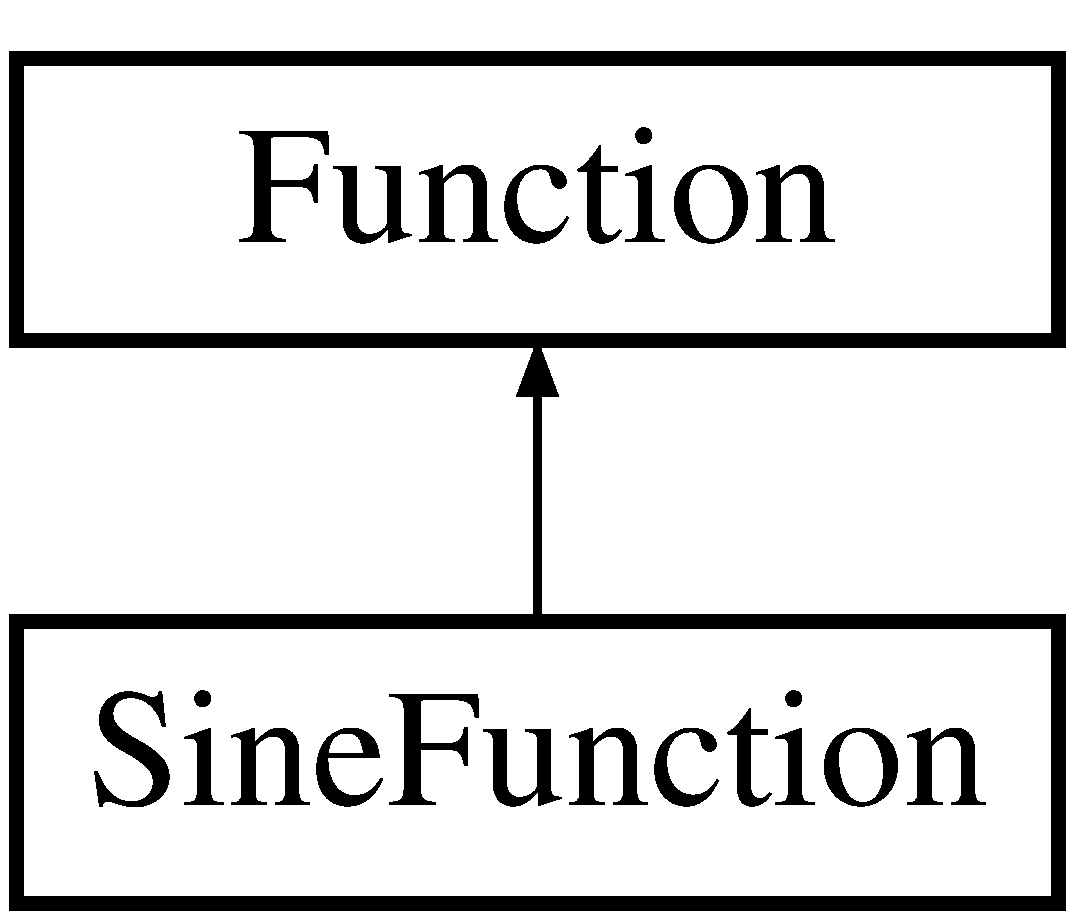
\includegraphics[height=2.000000cm]{class_sine_function}
\end{center}
\end{figure}
\subsection*{Public Member Functions}
\begin{DoxyCompactItemize}
\item 
virtual Decimal \hyperlink{class_sine_function_a551d6f4e81a2cdc03c185260a0738a10}{value\+At} (Decimal x) const 
\begin{DoxyCompactList}\small\item\em Method to determine the value of \hyperlink{class_sine_function}{Sine\+Function}. \end{DoxyCompactList}\end{DoxyCompactItemize}


\subsection{Detailed Description}
\hyperlink{class_function}{Function} to compute the sine of the input. 

\subsection{Member Function Documentation}
\hypertarget{class_sine_function_a551d6f4e81a2cdc03c185260a0738a10}{\index{Sine\+Function@{Sine\+Function}!value\+At@{value\+At}}
\index{value\+At@{value\+At}!Sine\+Function@{Sine\+Function}}
\subsubsection[{value\+At}]{\setlength{\rightskip}{0pt plus 5cm}virtual Decimal Sine\+Function\+::value\+At (
\begin{DoxyParamCaption}
\item[{Decimal}]{x}
\end{DoxyParamCaption}
) const\hspace{0.3cm}{\ttfamily [inline]}, {\ttfamily [virtual]}}}\label{class_sine_function_a551d6f4e81a2cdc03c185260a0738a10}


Method to determine the value of \hyperlink{class_sine_function}{Sine\+Function}. 

\begin{DoxyReturn}{Returns}
The sine of {\itshape x}. 
\end{DoxyReturn}


Implements \hyperlink{class_function_a7773feae8f1def0a2d7e479363700816}{Function}.



The documentation for this class was generated from the following file\+:\begin{DoxyCompactItemize}
\item 
Function.\+h\end{DoxyCompactItemize}

\hypertarget{class_square_root_function}{\section{Square\+Root\+Function Class Reference}
\label{class_square_root_function}\index{Square\+Root\+Function@{Square\+Root\+Function}}
}


\hyperlink{class_function}{Function} to compute the square root of the input.  




{\ttfamily \#include $<$Function.\+h$>$}

Inheritance diagram for Square\+Root\+Function\+:\begin{figure}[H]
\begin{center}
\leavevmode
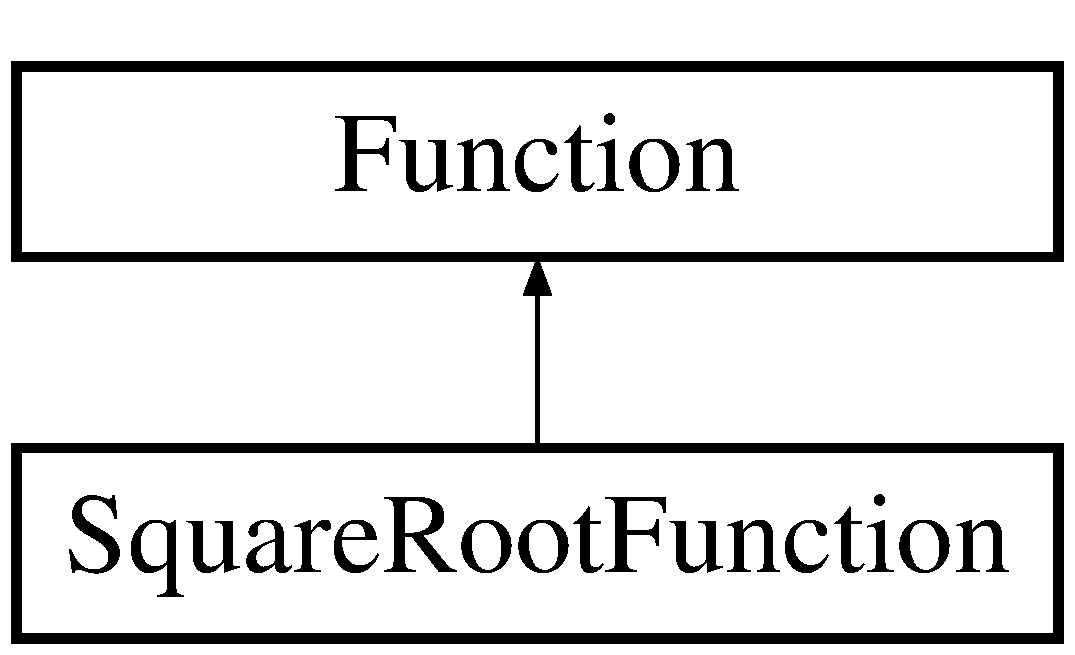
\includegraphics[height=2.000000cm]{class_square_root_function}
\end{center}
\end{figure}
\subsection*{Public Member Functions}
\begin{DoxyCompactItemize}
\item 
virtual Decimal \hyperlink{class_square_root_function_a6044091d737d7bd72325621c2dc56a7a}{value\+At} (Decimal x) const 
\begin{DoxyCompactList}\small\item\em Method to determine the value of \hyperlink{class_square_root_function}{Square\+Root\+Function}. \end{DoxyCompactList}\end{DoxyCompactItemize}


\subsection{Detailed Description}
\hyperlink{class_function}{Function} to compute the square root of the input. 

\subsection{Member Function Documentation}
\hypertarget{class_square_root_function_a6044091d737d7bd72325621c2dc56a7a}{\index{Square\+Root\+Function@{Square\+Root\+Function}!value\+At@{value\+At}}
\index{value\+At@{value\+At}!Square\+Root\+Function@{Square\+Root\+Function}}
\subsubsection[{value\+At}]{\setlength{\rightskip}{0pt plus 5cm}virtual Decimal Square\+Root\+Function\+::value\+At (
\begin{DoxyParamCaption}
\item[{Decimal}]{x}
\end{DoxyParamCaption}
) const\hspace{0.3cm}{\ttfamily [inline]}, {\ttfamily [virtual]}}}\label{class_square_root_function_a6044091d737d7bd72325621c2dc56a7a}


Method to determine the value of \hyperlink{class_square_root_function}{Square\+Root\+Function}. 

\begin{DoxyReturn}{Returns}
The square root of {\itshape x}. 
\end{DoxyReturn}


Implements \hyperlink{class_function_a7773feae8f1def0a2d7e479363700816}{Function}.



The documentation for this class was generated from the following file\+:\begin{DoxyCompactItemize}
\item 
Function.\+h\end{DoxyCompactItemize}

\hypertarget{class_tangent_function}{\section{Tangent\+Function Class Reference}
\label{class_tangent_function}\index{Tangent\+Function@{Tangent\+Function}}
}


\hyperlink{class_function}{Function} to compute the tangent of the input.  




{\ttfamily \#include $<$Function.\+h$>$}

Inheritance diagram for Tangent\+Function\+:\begin{figure}[H]
\begin{center}
\leavevmode
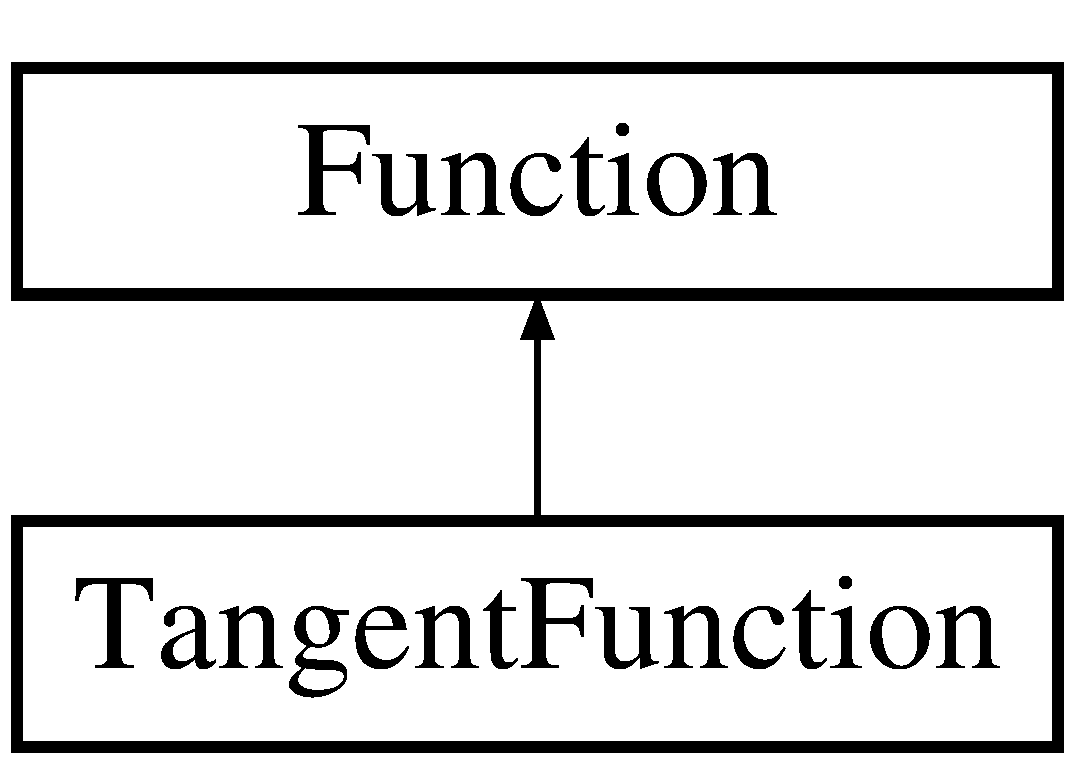
\includegraphics[height=2.000000cm]{class_tangent_function}
\end{center}
\end{figure}
\subsection*{Public Member Functions}
\begin{DoxyCompactItemize}
\item 
virtual Decimal \hyperlink{class_tangent_function_a1353a701417a2be51492d59276e5a5b7}{value\+At} (Decimal x) const 
\begin{DoxyCompactList}\small\item\em Method to determine the value of \hyperlink{class_tangent_function}{Tangent\+Function}. \end{DoxyCompactList}\end{DoxyCompactItemize}


\subsection{Detailed Description}
\hyperlink{class_function}{Function} to compute the tangent of the input. 

\subsection{Member Function Documentation}
\hypertarget{class_tangent_function_a1353a701417a2be51492d59276e5a5b7}{\index{Tangent\+Function@{Tangent\+Function}!value\+At@{value\+At}}
\index{value\+At@{value\+At}!Tangent\+Function@{Tangent\+Function}}
\subsubsection[{value\+At}]{\setlength{\rightskip}{0pt plus 5cm}virtual Decimal Tangent\+Function\+::value\+At (
\begin{DoxyParamCaption}
\item[{Decimal}]{x}
\end{DoxyParamCaption}
) const\hspace{0.3cm}{\ttfamily [inline]}, {\ttfamily [virtual]}}}\label{class_tangent_function_a1353a701417a2be51492d59276e5a5b7}


Method to determine the value of \hyperlink{class_tangent_function}{Tangent\+Function}. 

\begin{DoxyReturn}{Returns}
The tangent of {\itshape x}. 
\end{DoxyReturn}


Implements \hyperlink{class_function_a7773feae8f1def0a2d7e479363700816}{Function}.



The documentation for this class was generated from the following file\+:\begin{DoxyCompactItemize}
\item 
Function.\+h\end{DoxyCompactItemize}

\hypertarget{class_text}{\section{Text Class Reference}
\label{class_text}\index{Text@{Text}}
}


Draw a string of text.  




{\ttfamily \#include $<$Text.\+h$>$}

Inheritance diagram for Text\+:\begin{figure}[H]
\begin{center}
\leavevmode
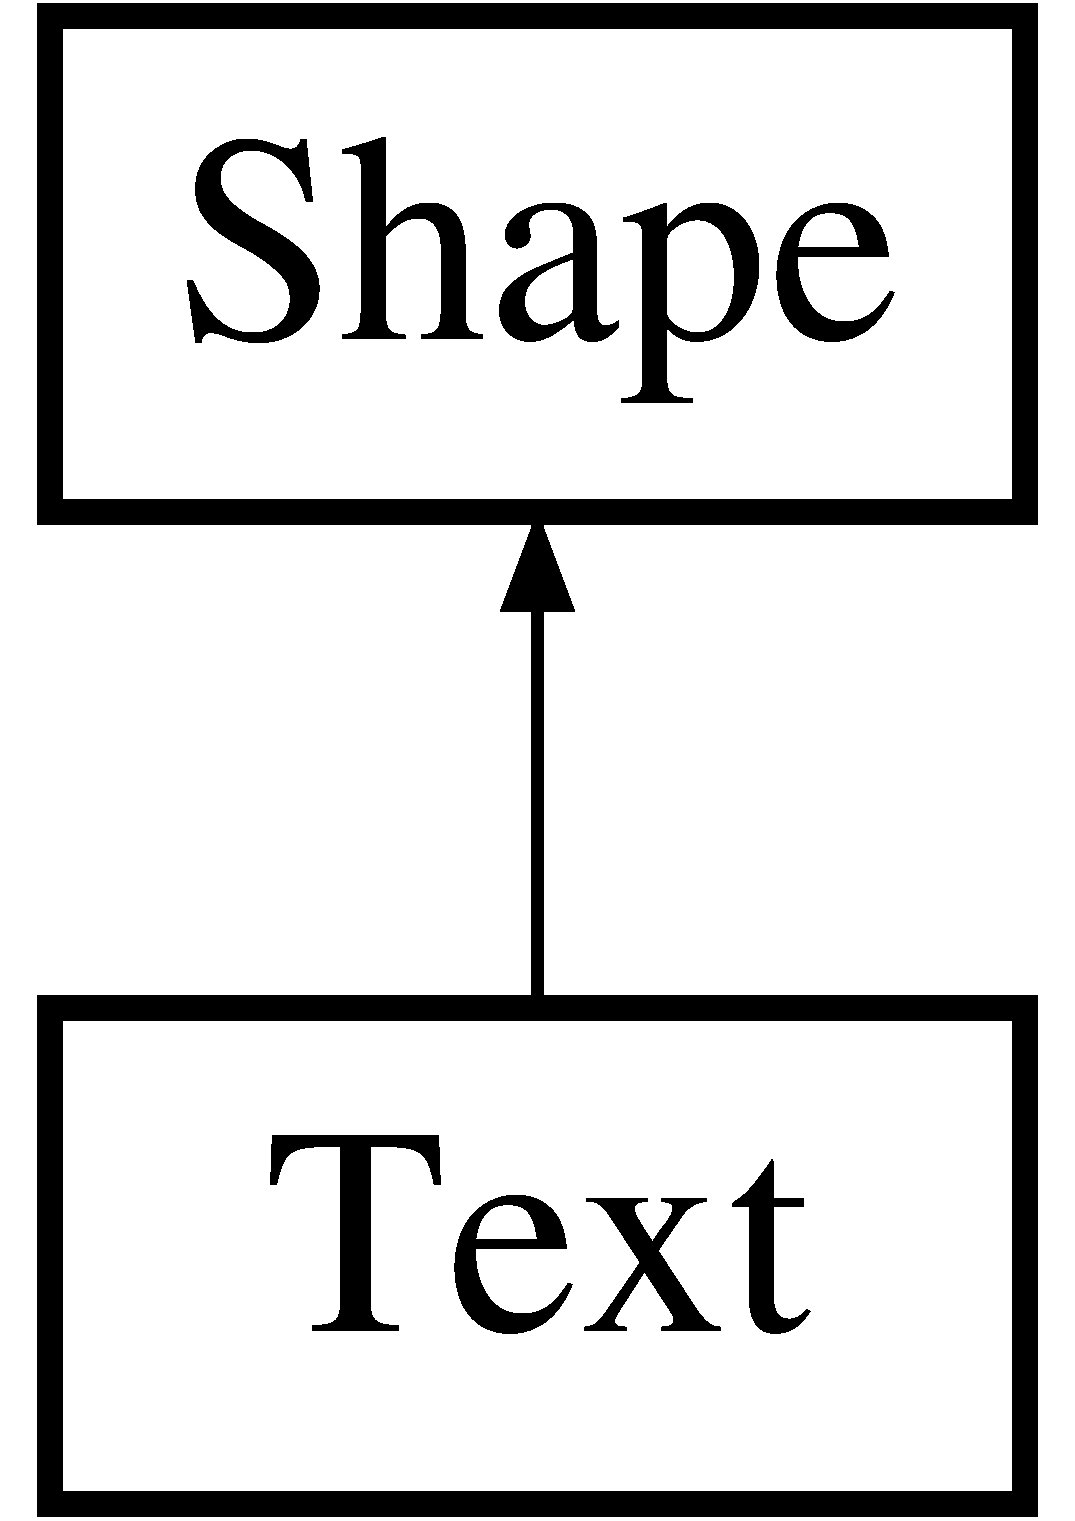
\includegraphics[height=2.000000cm]{class_text}
\end{center}
\end{figure}
\subsection*{Public Member Functions}
\begin{DoxyCompactItemize}
\item 
\hyperlink{class_text_a5f1ef9ca6779f8a01ea78442e4280f55}{Text} (std\+::wstring s, Texture\+Handler \&loader, int x, int y, unsigned int size, const \hyperlink{struct_color_float}{Color\+Float} \&color)
\begin{DoxyCompactList}\small\item\em Explicitly constructs a new \hyperlink{class_text}{Text} instance. \end{DoxyCompactList}\item 
void \hyperlink{class_text_adedc069a9ad622bf9d2cf6d194a01b39}{draw} ()
\begin{DoxyCompactList}\small\item\em Draw the \hyperlink{class_text}{Text}. \end{DoxyCompactList}\end{DoxyCompactItemize}
\subsection*{Additional Inherited Members}


\subsection{Detailed Description}
Draw a string of text. 

\hyperlink{class_text}{Text} is a class for holding the data necessary for rendering a string of text. \begin{DoxyNote}{Note}
\hyperlink{class_text}{Text} is aligned by the upper-\/left corner. 

At the moment, only a single font is supported. 
\end{DoxyNote}


\subsection{Constructor \& Destructor Documentation}
\hypertarget{class_text_a5f1ef9ca6779f8a01ea78442e4280f55}{\index{Text@{Text}!Text@{Text}}
\index{Text@{Text}!Text@{Text}}
\subsubsection[{Text}]{\setlength{\rightskip}{0pt plus 5cm}Text\+::\+Text (
\begin{DoxyParamCaption}
\item[{std\+::wstring}]{s, }
\item[{Texture\+Handler \&}]{loader, }
\item[{int}]{x, }
\item[{int}]{y, }
\item[{unsigned int}]{size, }
\item[{const {\bf Color\+Float} \&}]{color}
\end{DoxyParamCaption}
)}}\label{class_text_a5f1ef9ca6779f8a01ea78442e4280f55}


Explicitly constructs a new \hyperlink{class_text}{Text} instance. 

This is the constructor for the \hyperlink{class_text}{Text} class. 
\begin{DoxyParams}{Parameters}
{\em s} & The string to draw. \\
\hline
{\em loader} & A pointer to the Texture\+Handler with which to load the font. \\
\hline
{\em x} & The x coordinate. \\
\hline
{\em y} & The y coordinate. \\
\hline
{\em size} & The size of the text in pixels. \\
\hline
{\em color} & A color. \\
\hline
\end{DoxyParams}
\begin{DoxyReturn}{Returns}
A new \hyperlink{class_text}{Text} instance with the specified string, position, and color. 
\end{DoxyReturn}


\subsection{Member Function Documentation}
\hypertarget{class_text_adedc069a9ad622bf9d2cf6d194a01b39}{\index{Text@{Text}!draw@{draw}}
\index{draw@{draw}!Text@{Text}}
\subsubsection[{draw}]{\setlength{\rightskip}{0pt plus 5cm}void Text\+::draw (
\begin{DoxyParamCaption}
{}
\end{DoxyParamCaption}
)\hspace{0.3cm}{\ttfamily [virtual]}}}\label{class_text_adedc069a9ad622bf9d2cf6d194a01b39}


Draw the \hyperlink{class_text}{Text}. 

This function actually draws the \hyperlink{class_text}{Text} to the \hyperlink{class_canvas}{Canvas}. 

Implements \hyperlink{class_shape_afacc5aad8e37308c3ce8fef768199b05}{Shape}.



The documentation for this class was generated from the following files\+:\begin{DoxyCompactItemize}
\item 
Text.\+h\item 
Text.\+cpp\end{DoxyCompactItemize}

\hypertarget{class_timer}{\section{Timer Class Reference}
\label{class_timer}\index{Timer@{Timer}}
}


A class for various timing operations.  




{\ttfamily \#include $<$Timer.\+h$>$}

\subsection*{Public Member Functions}
\begin{DoxyCompactItemize}
\item 
\hyperlink{class_timer_aa9efcdd947c18f71b15205162483c79c}{Timer} (double period)
\begin{DoxyCompactList}\small\item\em Constructs a new \hyperlink{class_timer}{Timer}. \end{DoxyCompactList}\item 
\hypertarget{class_timer_a14fa469c4c295c5fa6e66a4ad1092146}{virtual \hyperlink{class_timer_a14fa469c4c295c5fa6e66a4ad1092146}{$\sim$\+Timer} ()}\label{class_timer_a14fa469c4c295c5fa6e66a4ad1092146}

\begin{DoxyCompactList}\small\item\em Destructor for the \hyperlink{class_timer}{Timer} class. \end{DoxyCompactList}\item 
unsigned int \hyperlink{class_timer_ab7c94a5d0f7d1e3a0a2370c9bc5f68f3}{get\+Reps} () const 
\begin{DoxyCompactList}\small\item\em Get the number of repetitions since start. \end{DoxyCompactList}\item 
double \hyperlink{class_timer_a8a1e22b1647df0f43d98cbfa1278a210}{get\+Time} () const 
\begin{DoxyCompactList}\small\item\em Get the elapsed time since starting the timer. \end{DoxyCompactList}\item 
double \hyperlink{class_timer_a354cf2011ae82fdb28011bb544e87307}{get\+Time\+Between\+Sleeps} () const 
\begin{DoxyCompactList}\small\item\em Get the elapsed time between sleeps. \end{DoxyCompactList}\item 
bool \hyperlink{class_timer_a1843db617c4da5826e0dd709b259bdb4}{past\+Period} ()
\begin{DoxyCompactList}\small\item\em Check if the timer's period has elapsed. \end{DoxyCompactList}\item 
void \hyperlink{class_timer_a7f1c5a4ef711075eec9a42afb6204a25}{reset} (double period=0)
\begin{DoxyCompactList}\small\item\em Reset the \hyperlink{class_timer}{Timer}. \end{DoxyCompactList}\item 
void \hyperlink{class_timer_a6b3d6e79d249b567a71104c4091d652f}{sleep} ()
\begin{DoxyCompactList}\small\item\em Sleeps the timer's current thread until its period elapses. \end{DoxyCompactList}\end{DoxyCompactItemize}
\subsection*{Static Public Member Functions}
\begin{DoxyCompactItemize}
\item 
static void \hyperlink{class_timer_aed9d38e6cefef77017f990558ae72ebb}{thread\+Sleep\+For} (double duration)
\begin{DoxyCompactList}\small\item\em Sleeps the current thread for the specified duration. \end{DoxyCompactList}\end{DoxyCompactItemize}


\subsection{Detailed Description}
A class for various timing operations. 

\hyperlink{class_timer}{Timer} provides a simple timer for timing, sleeping threads, and keeping track of the current rendering frame. 

\subsection{Constructor \& Destructor Documentation}
\hypertarget{class_timer_aa9efcdd947c18f71b15205162483c79c}{\index{Timer@{Timer}!Timer@{Timer}}
\index{Timer@{Timer}!Timer@{Timer}}
\subsubsection[{Timer}]{\setlength{\rightskip}{0pt plus 5cm}Timer\+::\+Timer (
\begin{DoxyParamCaption}
\item[{double}]{period}
\end{DoxyParamCaption}
)}}\label{class_timer_aa9efcdd947c18f71b15205162483c79c}


Constructs a new \hyperlink{class_timer}{Timer}. 

This is the default constructor for the \hyperlink{class_timer}{Timer} class. 
\begin{DoxyParams}{Parameters}
{\em period} & Time in seconds specifying the maximum amount of time to sleep. \\
\hline
\end{DoxyParams}
\begin{DoxyReturn}{Returns}
A new \hyperlink{class_timer}{Timer} with the specified period. 
\end{DoxyReturn}


\subsection{Member Function Documentation}
\hypertarget{class_timer_ab7c94a5d0f7d1e3a0a2370c9bc5f68f3}{\index{Timer@{Timer}!get\+Reps@{get\+Reps}}
\index{get\+Reps@{get\+Reps}!Timer@{Timer}}
\subsubsection[{get\+Reps}]{\setlength{\rightskip}{0pt plus 5cm}unsigned int Timer\+::get\+Reps (
\begin{DoxyParamCaption}
{}
\end{DoxyParamCaption}
) const}}\label{class_timer_ab7c94a5d0f7d1e3a0a2370c9bc5f68f3}


Get the number of repetitions since start. 

This function returns the number of times the \hyperlink{class_timer}{Timer} instance's period has elapsed. \begin{DoxyReturn}{Returns}
The number of times the period has elapsed since the \hyperlink{class_timer}{Timer} has been started. 
\end{DoxyReturn}


Referenced by past\+Period().

\hypertarget{class_timer_a8a1e22b1647df0f43d98cbfa1278a210}{\index{Timer@{Timer}!get\+Time@{get\+Time}}
\index{get\+Time@{get\+Time}!Timer@{Timer}}
\subsubsection[{get\+Time}]{\setlength{\rightskip}{0pt plus 5cm}double Timer\+::get\+Time (
\begin{DoxyParamCaption}
{}
\end{DoxyParamCaption}
) const}}\label{class_timer_a8a1e22b1647df0f43d98cbfa1278a210}


Get the elapsed time since starting the timer. 

This function returns the time in seconds since the \hyperlink{class_timer}{Timer} has been started. \begin{DoxyReturn}{Returns}
The time in seconds since starting the \hyperlink{class_timer}{Timer}. 
\end{DoxyReturn}


Referenced by Canvas\+::get\+Time().

\hypertarget{class_timer_a354cf2011ae82fdb28011bb544e87307}{\index{Timer@{Timer}!get\+Time\+Between\+Sleeps@{get\+Time\+Between\+Sleeps}}
\index{get\+Time\+Between\+Sleeps@{get\+Time\+Between\+Sleeps}!Timer@{Timer}}
\subsubsection[{get\+Time\+Between\+Sleeps}]{\setlength{\rightskip}{0pt plus 5cm}double Timer\+::get\+Time\+Between\+Sleeps (
\begin{DoxyParamCaption}
{}
\end{DoxyParamCaption}
) const}}\label{class_timer_a354cf2011ae82fdb28011bb544e87307}


Get the elapsed time between sleeps. 

This function returns the time in seconds between the last two calls to \hyperlink{class_timer_a6b3d6e79d249b567a71104c4091d652f}{sleep()}. \begin{DoxyReturn}{Returns}
The time in seconds between the last two sleeps 
\end{DoxyReturn}
\hypertarget{class_timer_a1843db617c4da5826e0dd709b259bdb4}{\index{Timer@{Timer}!past\+Period@{past\+Period}}
\index{past\+Period@{past\+Period}!Timer@{Timer}}
\subsubsection[{past\+Period}]{\setlength{\rightskip}{0pt plus 5cm}bool Timer\+::past\+Period (
\begin{DoxyParamCaption}
{}
\end{DoxyParamCaption}
)}}\label{class_timer_a1843db617c4da5826e0dd709b259bdb4}


Check if the timer's period has elapsed. 

This function returns whether the period of the \hyperlink{class_timer}{Timer} has elapsed since the last time the function was called. \begin{DoxyReturn}{Returns}
True if at least {\itshape period} seconds have elapsed since the last call, false otherwise. 
\end{DoxyReturn}
\hypertarget{class_timer_a7f1c5a4ef711075eec9a42afb6204a25}{\index{Timer@{Timer}!reset@{reset}}
\index{reset@{reset}!Timer@{Timer}}
\subsubsection[{reset}]{\setlength{\rightskip}{0pt plus 5cm}void Timer\+::reset (
\begin{DoxyParamCaption}
\item[{double}]{period = {\ttfamily 0}}
\end{DoxyParamCaption}
)}}\label{class_timer_a7f1c5a4ef711075eec9a42afb6204a25}


Reset the \hyperlink{class_timer}{Timer}. 

This function resets the starting time, repetitions, and period of the timer. 
\begin{DoxyParams}{Parameters}
{\em period} & The new period for the \hyperlink{class_timer}{Timer}. Setting this less than or equal to 0 will keep the current period. \\
\hline
\end{DoxyParams}


Referenced by Timer().

\hypertarget{class_timer_a6b3d6e79d249b567a71104c4091d652f}{\index{Timer@{Timer}!sleep@{sleep}}
\index{sleep@{sleep}!Timer@{Timer}}
\subsubsection[{sleep}]{\setlength{\rightskip}{0pt plus 5cm}void Timer\+::sleep (
\begin{DoxyParamCaption}
{}
\end{DoxyParamCaption}
)}}\label{class_timer_a6b3d6e79d249b567a71104c4091d652f}


Sleeps the timer's current thread until its period elapses. 

This function tells the currently executing thread to sleep until the rest of the \hyperlink{class_timer}{Timer} instance's remaining period expires.

If the timer's period has elapsed since last call, the thread will continue execution normally until the next call to \hyperlink{class_timer_a6b3d6e79d249b567a71104c4091d652f}{sleep()}. \begin{DoxyNote}{Note}
This function does not guarantee the thread will resume immediately after the time expires. Depending on your O\+S, the thread may sleep for longer. 
\end{DoxyNote}
\hypertarget{class_timer_aed9d38e6cefef77017f990558ae72ebb}{\index{Timer@{Timer}!thread\+Sleep\+For@{thread\+Sleep\+For}}
\index{thread\+Sleep\+For@{thread\+Sleep\+For}!Timer@{Timer}}
\subsubsection[{thread\+Sleep\+For}]{\setlength{\rightskip}{0pt plus 5cm}void Timer\+::thread\+Sleep\+For (
\begin{DoxyParamCaption}
\item[{double}]{duration}
\end{DoxyParamCaption}
)\hspace{0.3cm}{\ttfamily [static]}}}\label{class_timer_aed9d38e6cefef77017f990558ae72ebb}


Sleeps the current thread for the specified duration. 

This function tells the currently executing thread to sleep for {\itshape duration} seconds. \begin{DoxyNote}{Note}
This function does not guarantee the thread will resume immediately after {\itshape duration} expires. Depending on your O\+S, the thread may sleep for longer. 
\end{DoxyNote}


The documentation for this class was generated from the following files\+:\begin{DoxyCompactItemize}
\item 
Timer.\+h\item 
Timer.\+cpp\end{DoxyCompactItemize}

\hypertarget{class_triangle}{\section{Triangle Class Reference}
\label{class_triangle}\index{Triangle@{Triangle}}
}


Draw a simple \hyperlink{class_triangle}{Triangle}.  




{\ttfamily \#include $<$Triangle.\+h$>$}

Inheritance diagram for Triangle\+:\begin{figure}[H]
\begin{center}
\leavevmode
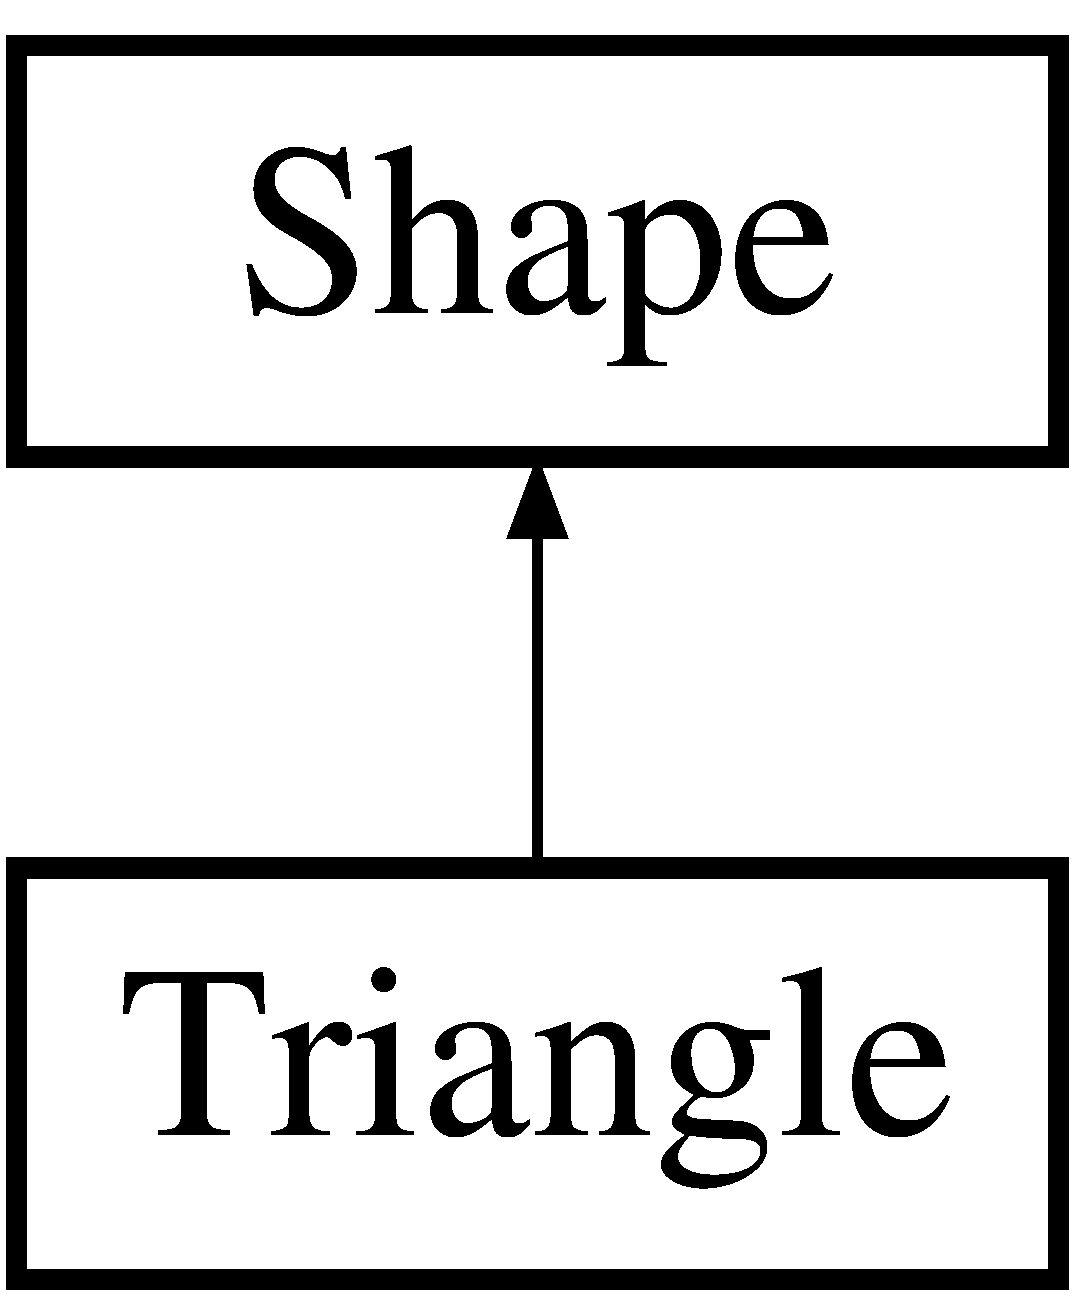
\includegraphics[height=2.000000cm]{class_triangle}
\end{center}
\end{figure}
\subsection*{Public Member Functions}
\begin{DoxyCompactItemize}
\item 
\hyperlink{class_triangle_a22609a1523399fd46fa3751afe692a1d}{Triangle} (int x1, int y1, int x2, int y2, int x3, int y3, const \hyperlink{struct_color_float}{Color\+Float} \&color)
\begin{DoxyCompactList}\small\item\em Explicitly constructs a new \hyperlink{class_triangle}{Triangle}. \end{DoxyCompactList}\item 
void \hyperlink{class_triangle_a43067ba4ee3c1d56930a567cc2186624}{draw} ()
\begin{DoxyCompactList}\small\item\em Draw the \hyperlink{class_triangle}{Triangle}. \end{DoxyCompactList}\end{DoxyCompactItemize}
\subsection*{Additional Inherited Members}


\subsection{Detailed Description}
Draw a simple \hyperlink{class_triangle}{Triangle}. 

\hyperlink{class_triangle}{Triangle} is a class for holding vertex data for a simple triangle. 

\subsection{Constructor \& Destructor Documentation}
\hypertarget{class_triangle_a22609a1523399fd46fa3751afe692a1d}{\index{Triangle@{Triangle}!Triangle@{Triangle}}
\index{Triangle@{Triangle}!Triangle@{Triangle}}
\subsubsection[{Triangle}]{\setlength{\rightskip}{0pt plus 5cm}Triangle\+::\+Triangle (
\begin{DoxyParamCaption}
\item[{int}]{x1, }
\item[{int}]{y1, }
\item[{int}]{x2, }
\item[{int}]{y2, }
\item[{int}]{x3, }
\item[{int}]{y3, }
\item[{const {\bf Color\+Float} \&}]{color}
\end{DoxyParamCaption}
)}}\label{class_triangle_a22609a1523399fd46fa3751afe692a1d}


Explicitly constructs a new \hyperlink{class_triangle}{Triangle}. 

This is the constructor for the \hyperlink{class_triangle}{Triangle} class. 
\begin{DoxyParams}{Parameters}
{\em x1} & The x coordinate of the first endpoint. \\
\hline
{\em y1} & The y coordinate of the first endpoint. \\
\hline
{\em x2} & The x coordinate of the second endpoint. \\
\hline
{\em y2} & The y coordinate of the second endpoint. \\
\hline
{\em x3} & The x coordinate of the second endpoint. \\
\hline
{\em y3} & The y coordinate of the second endpoint. \\
\hline
{\em color} & The color of the \hyperlink{class_triangle}{Triangle}. \\
\hline
\end{DoxyParams}
\begin{DoxyReturn}{Returns}
A new \hyperlink{class_triangle}{Triangle} with the specified vertices and color. 
\end{DoxyReturn}


\subsection{Member Function Documentation}
\hypertarget{class_triangle_a43067ba4ee3c1d56930a567cc2186624}{\index{Triangle@{Triangle}!draw@{draw}}
\index{draw@{draw}!Triangle@{Triangle}}
\subsubsection[{draw}]{\setlength{\rightskip}{0pt plus 5cm}void Triangle\+::draw (
\begin{DoxyParamCaption}
{}
\end{DoxyParamCaption}
)\hspace{0.3cm}{\ttfamily [virtual]}}}\label{class_triangle_a43067ba4ee3c1d56930a567cc2186624}


Draw the \hyperlink{class_triangle}{Triangle}. 

This function actually draws the \hyperlink{class_triangle}{Triangle} to the \hyperlink{class_canvas}{Canvas}. 

Implements \hyperlink{class_shape_afacc5aad8e37308c3ce8fef768199b05}{Shape}.



The documentation for this class was generated from the following files\+:\begin{DoxyCompactItemize}
\item 
Triangle.\+h\item 
Triangle.\+cpp\end{DoxyCompactItemize}

%--- End generated contents ---

% Index
\newpage
\phantomsection
\addcontentsline{toc}{chapter}{Index}
\printindex

\end{document}
